\documentclass{report}

\title{A Performance Evaluation of Task Parallelism on Intel Xeon and Xeon Phi}
\date{2015-09}
\author{Tom Farmer}

\usepackage{amsmath}
\usepackage{cite}
\usepackage{fixltx2e}
\usepackage{graphicx}
\usepackage{setspace}
\usepackage[top=2.5cm, bottom=2.5cm, left=3.2cm, right=2.5cm]{geometry}

%necessary for underscores in headings
\usepackage{url}
\urlstyle{same} % omit this command if you want monospaced-font look
\newcommand\purl[1]{\protect\url{#1}} % "protected url"

\def\changemargin#1#2{\list{}{\rightmargin#2\leftmargin#1}\item[]}
\let\endchangemargin=\endlist 

\newenvironment{mono}{\fontfamily{ttfamily}\selectfont}{\par}

\newenvironment{embedcode}{\begin{changemargin}{6em}{3em}\begin{mono}{}}{\end{mono}\end{changemargin}}

\begin{document}
\pagenumbering{gobble}
%\maketitle

\begin{titlepage}
\begin{center}
\newcommand{\HRule}{\rule{\linewidth}{0.5mm}}
% Upper part of the page. The '~' is needed because \\
% only works if a paragraph has started.

\includegraphics[width=0.5\textwidth]{./SwanseaLogo}~\\[1cm]

% Title
\HRule \\[0.4cm]
{ 
\huge \bfseries A Performance Evaluation of Task Parallelism on Intel Xeon and Xeon Phi \\[0.4cm]
}

\HRule \\[1.5cm]

\begin{center}

% Author and supervisor
\noindent
\emph{\large Author:}\\[0.1cm]
{\Large Thomas Farmer}\\[0.1cm]
Student number: 809130\\[0.5cm]
\emph{\large Supervisor:} \\[0.1cm]
{\Large Dr. Benjamin Mora}\\[6.0cm]

Project Dissertation submitted to Swansea University in Partial\\ Fulfilment for the Degree of Master of Science\\[0.5cm]

Department of Computer Science, Swansea University

\end{center}

\vfill

% Bottom of the page
{\large September 2015}

\end{center}

\clearpage

\end{titlepage}

\newpage

\onehalfspacing
\begin{abstract}
Task parallelism is a well-known approach to writing parallel applications, but literature evaluating frameworks providing support for task parallelism on modern hardware is rare. In this report, four benchmarks are developed to evaluate the performance of task parallelism on the Intel Xeon processor and Intel Xeon Phi coprocessor. Two common task parallelism frameworks, Cilk Plus and OpenMP, are tested against serial implementations of the same benchmarks to help produce recommendations for maximising performance of task parallel applications. The granularity of tasks is found to be a key aspect in achieving peak performance, while other factors reported in the literature, such as automatic vectorisation, are found to be less important. For small work-loads, the host machine containing two Xeon processors is found to outperform a single Xeon Phi coprocessor, but this difference is found to be less severe when the work-load increases.
\end{abstract}

\newpage
\begin{center}
{\huge Declaration}
\end{center}
\hfill
\newline
\newline

\noindent
DECLARATION\\
This work has not previously been accepted in substance for any degree and is not being concurrently submitted in candidature for any degree.
\newline
\newline
\newline

\noindent
STATEMENT 1\\
This dissertation is the result of my own independent work/investigation, except where otherwise stated. Other sources are acknowledged by giving explicit references. A bibliography is appended.
\newline
\newline
\newline

\noindent
STATEMENT 2\\
I hereby give consent for my dissertation, if accepted, to be available for photocopying and for inter-library loan, and for the title and summary to be made available to outside organisations.
\newline
\newline
\newline
\newline
\begin{center}
SIGNATURE \hspace{20em} DATE
\end{center}

\newpage
\begin{center}
{\huge Acknowledgements}
\end{center}
\hfill
\newline
\newline

\noindent
My sincere gratitude goes to Dr. Ben Mora for his help and advice throughout this project and to Dr. Jens Blanck for his valuable feedback on earlier reports. I am also grateful to my parents for funding my tuition.

\singlespacing
\newpage
\tableofcontents
\newpage
\listoffigures
\newpage
\pagenumbering{arabic}
\onehalfspacing

\chapter{Introduction} \label{Sec:introduction}

Multithreaded programs often do not produce a linear performance improvement over their serial counterparts. Overhead related to thread management, such as initialising threads and allotting them work, has been identified as a cause of this phenomenon, but hardware constraints like memory bandwidth and communication latency between processing cores also play a role\cite{Andrews99}. Task parallelism is an alternative to thread-centric parallelism which divides computations into so-called `tasks' and leaves the management of those tasks to a specialised scheduler\cite{Andrews99}. This approach is claimed to ease the process of developing some classes of parallel applications, especially including those featuring recursion or significant work-load imbalance\cite{Olivier09}. This project will evaluate the performance of two popular task-parallelism frameworks, Cilk Plus and OpenMP, on different hardware using a set of carefully selected benchmarks including a Fibonacci program, a parallel merge sort, a solution to the N-Queens puzzle and the Unbalanced Tree Search (UTS) artificial benchmark. Particular attention is paid in the evaluation of the results to potential hardware or software explanations for the presence of particular features, with the intention of providing recommendations for maximising parallel performance when writing applications that make use of task parallelism.

\section{Motivation} \label{Sec:motivation}

While the literature contains many analyses of various task parallelism frameworks and hardware devices, the usefulness of these reports is limited by a number of factors. Literature on OpenMP as a whole is widely available, but benchmarks conducted with its relatively new tasking capabilities are less common. Likewise, Intel's recent purchase of Cilk means that reports testing the latest version, Cilk Plus, are not as common as those testing earlier versions. In addition, some of the available studies evaluate the performance of these frameworks on only one hardware device, producing results that fail to control for differences in hardware \cite{Duran09}. It is hoped that running similar benchmarks on mainstream Intel hardware will provide more useful results.

\section{Methodology} \label{Sec:methodology}

Some authors have performed evaluations of the technologies used in this project by producing large, practical programs with real-world applications such as chess engines and scientific software\cite{Dailey01}. In this project, a set of benchmarks is developed in the hope that more, smaller, programs will produce results from which more insight may be gained. A key part of this approach is a thorough evaluation; the aim is to identify features in the data that may be caused by certain aspects of the technologies being tested.

Cilk Plus and OpenMP 3.0 are available as both C as Fortran extensions, but the benchmarks for this project are developed in C due to the overwhelming use of that language in the literature. Testing a selection of different C compilers may be also produce useful results, but this report is limited to evaluating the performance of the benchmarks when compiled with the Intel C++ Compiler (icc). icc supports all the necessary features of both frameworks, while popular alternatives like GCC have either incomplete support for some features, or only have full support in recent versions not available on the systems used to compile the benchmarks. All benchmarks are run on both an Intel Xeon Phi and the host machine which houses it. This is intended to help clarify which features are caused by hardware and which by the frameworks or benchmarks themselves.

\section{Goals} \label{Sec:goals}

With the motivation and approach outlined above, the intended goals of this project are as follows:
\begin{itemize}
	\item Select a set of benchmarks from the literature that strain particular aspects of the technologies under test in a variety of ways.
	\item Develop a serial version of each benchmark to serve as a basis for comparison.
	\item Develop task parallel versions of the benchmarks with Cilk Plus and OpenMP 3.0.
	\item Generate broad and detailed data sets by running the benchmarks using the technologies under test, from which useful conclusions may be drawn.
	\item Produce detailed figures for each combinations of technologies to facilitate identification of particular hardware and software features and allow comparison between alternative approaches.
	\item Conduct an evaluation of the data, with the aim of identifying performance characteristics of the benchmarks, their serial and parallel implementations, and the Xeon Phi and host machine on which they are run.
	\item Develop a set of recommendations for maximising performance of task parallelism on Intel Xeon and Xeon Phi.
\end{itemize}

\section{Chapters} \label{Sec:chapters}

Chapter 2 contains background information related to parallel applications and task parallelism in particular. The features of Cilk Plus and OpenMP are described in detail, with reference to the benchmark implementations included in the appendix. The architecture of the test hardware is also described to ensure an understanding of factors that cause particular features to appear in the benchmark results. Chapter 3 describes the benchmarks used in this project, the motivation for their inclusion and details related to their implementation. A literature survey is also conducted for each benchmark to provide a point of comparison for the results obtained. Chapter 4 evaluates in detail the results of running the benchmarks on the host machine and Xeon Phi. Performance charts for each trial are included, as well as heatmaps intended to highlight additional features that may not appear in two-dimensional graphs. Chapter 5 summarises the evaluation and presents a set of recommendations for achieving greater performance when writing task parallel applications. An appraisal of the usefulness of the results is included, followed by commentary on improvements that could be made to the benchmarking methodology.

\chapter{Background} \label{Sec:background}

\section{Task Parallelism} \label{Sec:taskparallelism}

Concurrent programs differ from sequential programs in that they are divided into smaller parts that can be executed simultaneously as multiple processes in order to complete a computation\cite{Andrews99}. These processes are run on independent ``threads" that each execute processor instructions that contribute to solving a larger task. These threads may be executed on multiple, independent processors or processor cores if available. The low-level management of threads has traditionally been left to specialised libraries such as POSIX threads\cite{pthreads}, but higher-level alternatives like MPI and early versions of OpenMP have also found widespread use in industrial and scientific environments\cite{Hwang98}. However, for some applications, such as those making use of while-loops and recursive routines, this ``data parallelism" is not always the most convenient approach\cite{Ayguade09}. Task parallelism is an alternative to data parallelism that divides programs into ``tasks" that are then scheduled for execution on independent threads. This approach takes the scheduling of work out of the hands of the programmer, instead relying on an automated work scheduler to decide which tasks should be executed and when, and on which thread\cite{Ayguade09}. The two task parallelism frameworks used in this project are Cilk Plus and OpenMP 3.0\cite{Podobas15}, described in Sections \ref{Sec:cilkplus} and \ref{Sec:openmp}, respectively.

\section{Cilk Plus} \label{Sec:cilkplus}
     	
Cilk Plus is a programming language maintained by Intel that natively supports task parallelism through a small set of keywords. It also provides additional functionality such as reduction operations, parallel loops and array notation. `Cilk' refers to the original language developed by MIT, but it may also refer to the family of languages which have spawned from it. Although the original version of Cilk (sometimes called `MIT Cilk' to avoid confusion) was distributed as a Cilk-to-C converter, modern versions of Cilk, including Intel's Cilk Plus, manifest themselves as extensions to existing C/C++ compilers.

This original basis in ANSI C means that Cilk Plus programs appear as normal C/C++ programs with only the addition of the Cilk keywords: \verb!cilk_spawn!, \verb!cilk_sync! and \verb!cilk_for!. An interesting feature of this model, known as serial elision, is that removing the Cilk keywords from such a program yields a valid C/C++ program\cite{Jeffers13}. While the reverse is also true -- simple concurrency can be easily achieved by adding Cilk keywords to existing C/C++ programs -- this does not guarantee efficiency, and the correct usage of Cilk's features to gain effective and safe parallelism remains the responsibility of the programmer. In fact, Cilk Plus is not guaranteed to spawn new tasks when it encounters a keyword; the role of the keywords is to allow the programmer to highlight potential parallelism for the compiler, but ultimate control over the spawning of new tasks is handled by the Cilk implementation. Cilk's model of parallelism has been used with success in real-world applications, such as the *Socrates chess engine, which won third place at the 1994 ACM International Chess Championship\cite{Blumofe95}.

One of the Cilk's most notable features, and where it differs from OpenMP's implementation of task parallelism, is its work-stealing scheduler. Each worker maintains its own work queue to which new tasks are added. If a thread completes the work in its queue, it may steal work from another thread. Leiserson and Blumofe, two of Cilk's original developers, have shown this approach to be “provably good”\cite{Blumofe95}\cite{Leiserson97}. The work-stealing scheduler is explained in more detail in Section \ref{Sec:workstealingscheduler}.

\subsection{Using Cilk Plus} \label{Sec:usingcilkplus}

When using the Intel C++ Compiler (icc), Cilk Plus features can be accessed by including the Cilk header file in normal C/C++ code. The three core keywords used by Cilk Plus to describe the parallelism of a given program are \verb!cilk_spawn!, \verb!cilk_sync! and \verb!cilk_for!. \verb!cilk_spawn! is placed directly before a function call in the following way:

\begin{center}
{\ttfamily \verb!cilk_spawn! foo();}
\end{center}

This line tells the compiler that the \verb!foo! function can be executed in parallel with the calling function, and may spawn a new task, adding it to the work queue of the spawning thread\cite{Jeffers13}. Cilk does not have `fire-and-forget' tasks; all tasks spawned with \verb!cilk_spawn! can, and eventually must, be joined again with the current thread\cite{Jeffers13}.

\verb!cilk_sync! is used to rejoin all child tasks spawned from a given spawning block with their parent task\cite{Jeffers13}. It is not necessary to specify which tasks are to be synchronised. Any parallelism that the spawning block created is ended when \verb!cilk_sync! is encountered. Exiting a spawning block, such as a function or try block, always invokes an implicit synchronisation, but \verb!cilk_sync! is used explicitly throughout this project for clarity. A simple example using \verb!cilk_spawn! and \verb!cilk_sync! in C is shown below.

\begin{embedcode}
\begin{verbatim}
int getNumber() {
    return 42;
}

int example() {
    int number = cilk_spawn getNumber();
    cilk_sync;
    printf("%d", number”);
    return 0;
}
\end{verbatim}
\end{embedcode}

The \verb!getNumber! function is executed in another task, but \verb!example! does not proceed beyond the spawning of that task because of \verb!cilk_sync!. The number returned can then be used safely, because \verb!getNumber! is guaranteed to have returned before \verb!printf! is called.

\verb!cilk_for! is a substitute for the standard C for-loop, and allows the programmer to specify a parallel loop without spawning tasks manually. This has the advantage of minimising the effort needed to write Cilk programs, while simultaneously applying an efficient strategy for populating the work queues: the iterations of the loop are divided into two equal ranges and executed as new tasks, then further subdivided in the same way until the ranges are less than the “grain size” specified by the programmer\cite{cilkplussite}. \verb!cilk_for! is used in the N-Queens benchmark as part of a backtrack search algorithm, described in detail in Section \ref{Sec:nqueens}.

\verb!__cilkrts_set_param! is a function that allows the programmer to modify Cilk's behaviour with certain parameters; the Cilk Plus implementations of the benchmarks developed for this project make extensive use of the \verb!nworkers! parameter, which sets the number of threads Cilk's scheduler may use. Newer versions of Cilk also have built-in support for parallel reduction algorithms, but these are not used in this project.

\subsection{Work-Stealing Scheduler} \label{Sec:workstealingscheduler}

One of Cilk's key features is its ``work-stealing scheduler". Each thread maintains its own work queue, implemented as a double-ended queue, to which new tasks spawned on that thread are added\cite{Blumofe95}. If a thread completes all of the work in its queue, it becomes a ``thief", and steals work from the work queue of another, random thread, the ``victim". This approach to task scheduling has been shown repeatedly in the literature to have excellent load-balancing properties if the granularity of the tasks is designed carefully\cite{Tousimojarad14}. This contributes to the ability of Cilk Plus to achieve impressive parallel speedup, and is discussed extensively throughout Chapter \ref{Sec:evaluation}.

\section{OpenMP} \label{Sec:openmp}

OpenMP is an API that facilitates the development of parallel programs through compiler directives that create threads and distribute work to them\cite{openmpsite}. There are both C and Fortran versions, each with their own different, but similar, syntax. This section describes OpenMP and its features as they relate to C, the language used for the project. The features used in the implementation portion of this project appeared in the OpenMP 3.0 specification finalised in 2009\cite{openmpsite}, which introduced task parallelism in the form of the \verb!task! and \verb!taskwait! commands.

In C, the compiler directives used by OpenMP come in the form of pragmas, which are parsed at compile-time by the preprocessor to generate parallel code. Because potential parallelism is identified with pragmas, the compiler can safely ignore them and execute the program as if it were a serial implementation of the desired algorithm. In fact, the C standard explicitly states that any unrecognised pragmas should be ignored by the compiler\cite{Hook05}. This behaviour can be demonstrated by attempting to use icc to compile a program containing OpenMP pragmas, without the \verb!-fopenmp! flag that enables OpenMP functionality.

\subsection{Using OpenMP} \label{Sec:usingopenmp}

The Intel C++ Compiler supports the features of OpenMP 3.0 used in the implementation portion of this project. The basic features of OpenMP can be used without including any header files, but additional functionality can be accessed by including the \verb!omp.h! header\cite{Jeffers13}. OpenMP has a much more complex syntax than Cilk Plus because it supports other kinds of parallel programming constructs than task parallelism\cite{openmpspec}. It is therefore more complicated than the few Cilk Plus features described in Section \ref{Sec:usingcilkplus}, but the focus of this section is on the particular OpenMP features used in this project. 

All OpenMP constructs in C begin with \verb!#pragma omp!. If OpenMP is supported by the compiler, the preprocessor will parse the clauses attached to the pragma and, if possible, apply the parallelism they define to the next block. One of the most basic constructs is the \verb!#pragma omp parallel! construct, which indicates that the commands in the next block can be executed concurrently by multiple threads, called a team\cite{openmpspec}. Unlike Cilk Plus, which initialises its threads at the start of the program's execution, OpenMP initialises new threads whenever the parallel construct is encountered. For programs taking advantage of task parallelism, it is convenient to initialise all threads for a particular parallel section with a pragma that uses the parallel construct, and then use task-related commands within the enclosed block.

The parallel construct may be combined with the \verb!num_thread()! clause, which allows the programmer to specify how many threads are to be created. For example:

\begin{embedcode}
\begin{verbatim}
#pragma omp parallel num_threads(4)
{
    printf("Hello, world!");
}
\end{verbatim}
\end{embedcode}

This code specifies that the compiler can create four threads and execute the \verb!printf! function concurrently. It is also possible to predefine the number of threads to create with the \verb!omp_set_num_threads! function. This is how the number of threads to use is specified in the code for this project, because tedious recompilation is avoided by reading values from the command line when a given benchmark is executed and the number of threads set in the main function. OpenMP constructs may also be accompanied by clauses that specify the visibility of variables within the enclosed block, such as the \verb!shared! and \verb!firstprivate! clauses. These are used extensively in the benchmark implementations, although \verb!firstprivate! is sometimes implicit\cite{openmpspec}.

Within a parallel construct, the \verb!#pragma omp single! construct can be used to ensure that the code in the block that follows is executed on only one thread. In the OpenMP versions of the benchmarks developed in this project, the main function always contains the following code:

\begin{embedcode}
\begin{verbatim}
#pragma omp parallel
{
    #pragma omp single nowait
    {
        //...
    }
}
\end{verbatim}
\end{embedcode}

This parallel-single idiom allows the costly initialisation of many threads to occur before work is distributed to them, while ensuring that any tasks spawned within the parallel block are only spawned from a single thread. In this way, unnecessary duplication of work is avoided, but all of the threads initialised by the parallel construct are ready to be allocated tasks. The \verb!nowait! clause specifies that threads in the team created by the parallel construct should not wait for the thread executing the single block to finish before continuing beyond the single block\cite{openmpspec}.

Within the single block of the above code, or in a function called from within it, new tasks are spawned with \verb!#pragma omp task!. This is comparable with the \verb!cilk_spawn! command in Cilk Plus, but the command executed (such as a function call) is the line immediately following the pragma. The \verb!#pragma omp taskwait! pragma synchronises spawned tasks with the current thread, and is used in the same way as \verb!cilk_sync! in Cilk Plus. This is interesting to note because within the parallel and single constructs, the OpenMP and Cilk Plus implementation often look similar. Another feature, used in the N-Queens benchmark described in Section \ref{Sec:nqueens}, is the \verb!#pragma omp for! directive, which indicates that the standard C loop that follows can be executed in parallel by the current team.

Another feature used in the benchmarks is the \verb!kmp_set_defaults()! extension available on the Intel compiler, which is used with the \verb!“KMP_AFFINITY=...”! argument to specify how OpenMP threads map to the physical processor cores\cite{openmpaffinity}. The available thread affinity options are `compact', `scatter', `balanced' and `none'\cite{Wang14}. The compact affinity uses threads in the order they are numbered, so that OpenMP will use all of the threads in a single processor core before moving onto the next one\cite{Wang14}. The scatter affinity allocates threads to the least-used cores to achieve load balance\cite{Wang14}. The balanced affinity considers both load balance and data localisation when allocating threads to physical cores\cite{Wang14}. The performance of each of these options is benchmarked alongside setting no affinity is evaluated in Chapter \ref{Sec:evaluation} and the implications of these results discussed in Chapter \ref{Sec:conclusion}.

\subsection{Task Scheduling}

OpenMP schedules tasks at ``task scheduling points", which occur at particular locations defined by the OpenMP 3.0 specification\cite{openmpspec}. It does not define how scheduling is to be conducted, leaving this decision to individual implementations. Duran \textit{et al.}\cite{Duran09} evaluated the performance of several task scheduling strategies for OpenMP and found that work-first scheduling, in which threads that spawn new tasks suspend the current tasks and switch to executing the new one, was generally more performant than breadth-first scheduling, which places new tasks in a shared team pool from which threads can ``grab" tasks for execution. It should be noted that performance expectations should be based upon several factors, including the compiler used. The performance results discussed in Chapter \ref{Sec:evaluation} should therefore be considered to only apply to the Intel C++ Compiler.

\section{Intel Xeon and Xeon Phi} \label{Sec:intelxeonandxeonphi}

In order to perform a thorough and useful analysis of the results obtained from the benchmarks, it is necessary to understand the characteristics of the hardware on which they were run. The results from running the benchmarks developed for this project were obtained on two hardware devices/configurations:
\begin{itemize}
	\item A computer with two Intel Xeon processors (the ``host machine")
	\item A single Intel Xeon Phi coprocessor
\end{itemize}

This section describes the architecture of the Intel Xeon processor and Intel Xeon Phi coprocessor, as well as the configurations in which they were run. Background information related to processor design more generally is intentionally omitted in the interest of space. References to aspects of the hardware that may cause certain features to appear in the data are made throughout Chapter \ref{Sec:evaluation}.

\subsection{Intel Xeon and the Host Machine} \label{Sec:intelxeonandhost}

The ``host machine" is a computer containing two Intel Xeon E5-2660 processors in a dual-socket configuration connected by an Intel QuickPath Interconnect (QPI). Each Xeon is a 64-bit x86 processor featuring eight processing cores clocked at 2.2 GHz, and two hardware threads per core. Each core is connected by an on-die ring interconnect. Each core also contains 32 KB of instruction and 32 KB of data L1 cache, as well as 256 KB shared instruction/data L2 cache\cite{xeondatasheet}. 20 MB of L3 cache is shared between all cores\cite{xeonoverview}. A 256-bit vector unit is present on each core\cite{xeonoverview}. The host machine system contains 64 GB of DDR3 memory, which can be confirmed by running the \verb!free! command.
\noindent
\begin{figure}
	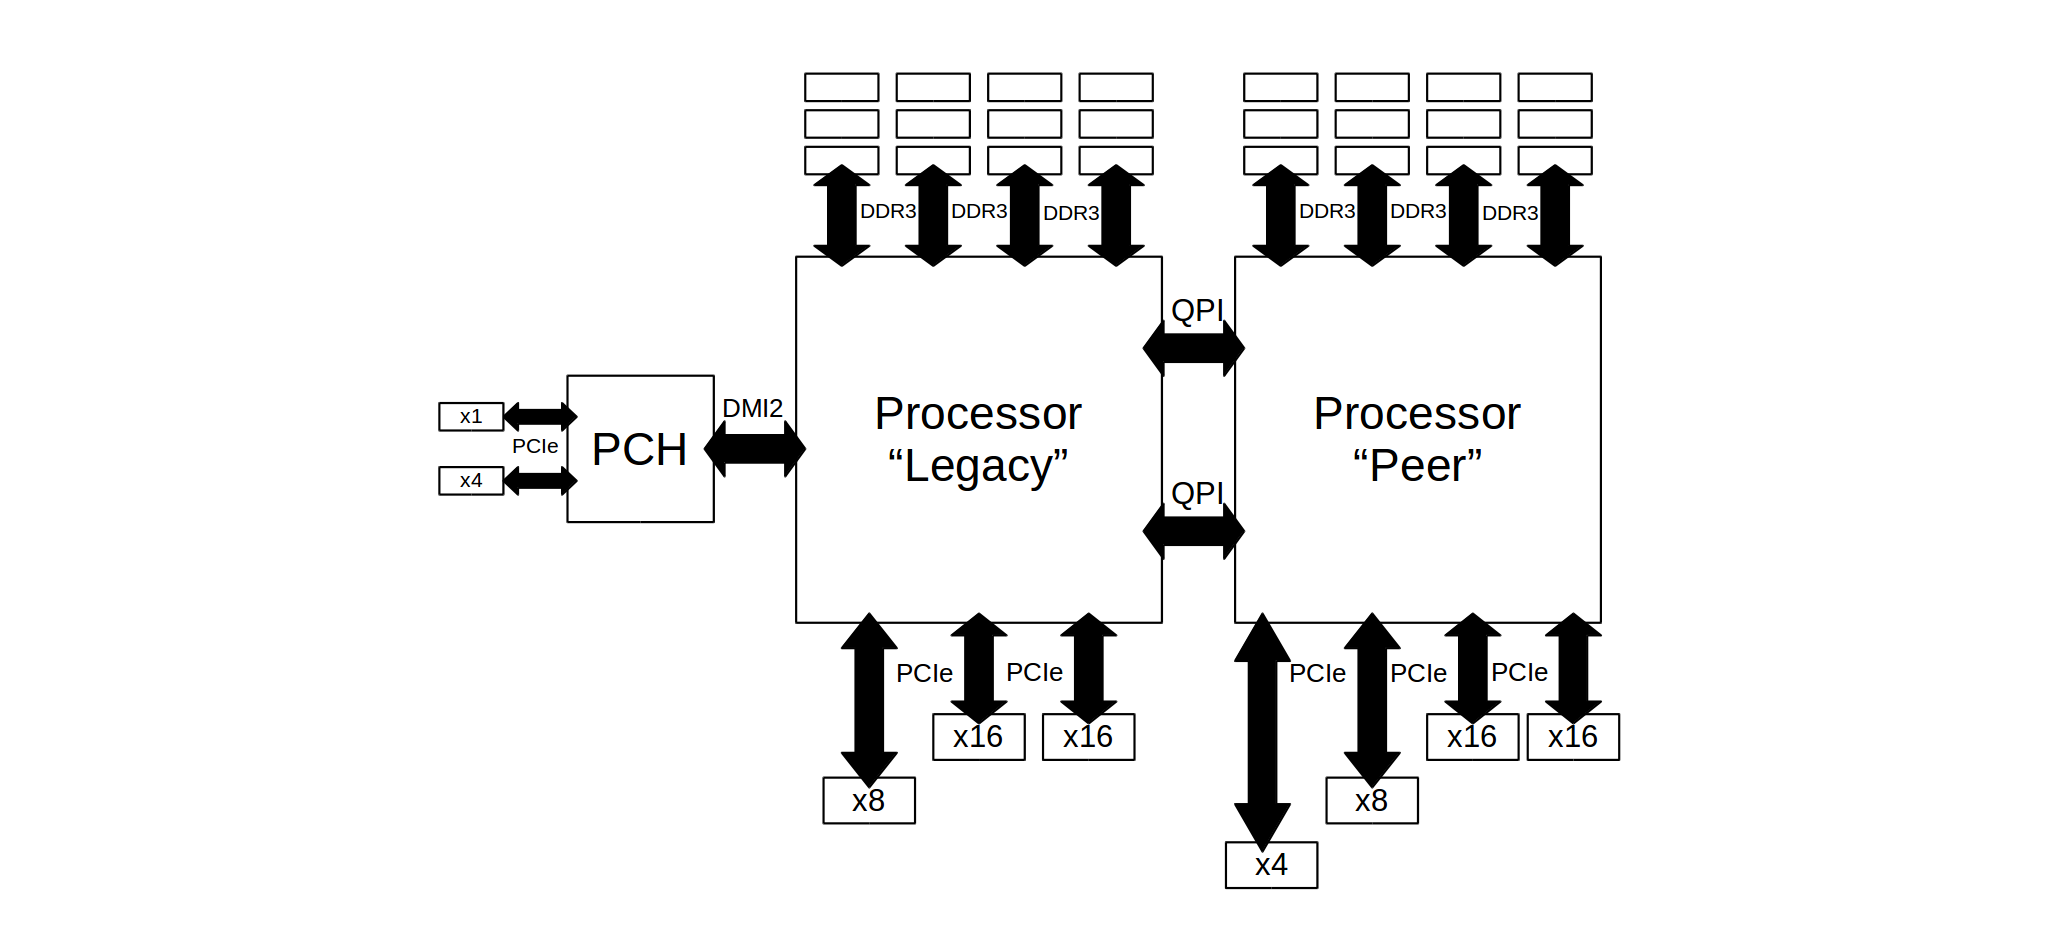
\includegraphics[width=\linewidth]{../diagrams/xeon}
	\caption{Intel Xeon Processor E5-2600 Product Family on the 2 Socket Platform\cite{xeondatasheet}.}
	\label{Fig:xeon}
\end{figure}

Figure \ref{Fig:xeon} shows the relationship between the Xeon processors and the PCI-E slots into which an Intel Xeon Phi card is inserted. The host machine contains four Xeon Phi cards, but only one was used in this project. It also shows the configuration of the two Xeon processors in the host machine. Running the \verb!lscpu! command reveals that the order of the 32 threads available are staggered across the two devices; the processor designated ``node0" executes threads 0-7 and 16-23 and ``node1" executes threads 8-15 and 24-31.

\subsection{Intel Xeon Phi} \label{Sec:intelxeonphi}

Intel's Many-Integrated Core (MIC) architecture attempts to overcome the communication overhead experienced by highly parallel computing clusters, which often communicate across a network, by placing dozens of processing cores on a single chip\cite{Jeffers13}. The chip is incorporated onto the surface of a PCI-E card and is used as a coprocessor in conjunction with Intel's Xeon processors. Instead of communicating across a network, the processing units of the Xeon Phi communicate locally through a fast ring interconnect, and share the card's built-in memory. This architecture allows the Xeon Phi to achieve unprecedented levels of parallel performance; the model used for this report is the 5110P (confirmed by running the \verb!micinfo! command on the host machine), which with 60 cores clocked at around 1.1 GHz, has a theoretical maximum performance of just over 2 TFLOPS\cite{Jeffers13}. The Xeon Phi was chosen for this project because it supports the highest degree of MIMD (Multiple Instruction, Multiple Data) parallelism of the available devices. Although only a single card is used in this project, the Xeon Phi also has the ability to operate in an ``offload" mode, in which work is allocated by the host machine to multiple cards\cite{Jeffers13}.

\subsubsection{Architecture} \label{Sec:phiarchitecture}

Intel Xeon Phi devices are coprocessors that can operate independently of the CPU. Each device is an SMP (Symmetric Multiprocessor) on-a-chip with a small amount of local flash memory which stores a minimal distribution of the Linux operating system\cite{Jeffers13}. The end-user can also use this memory to save their own files, such as program binaries or output data.
\noindent
\begin{figure}
	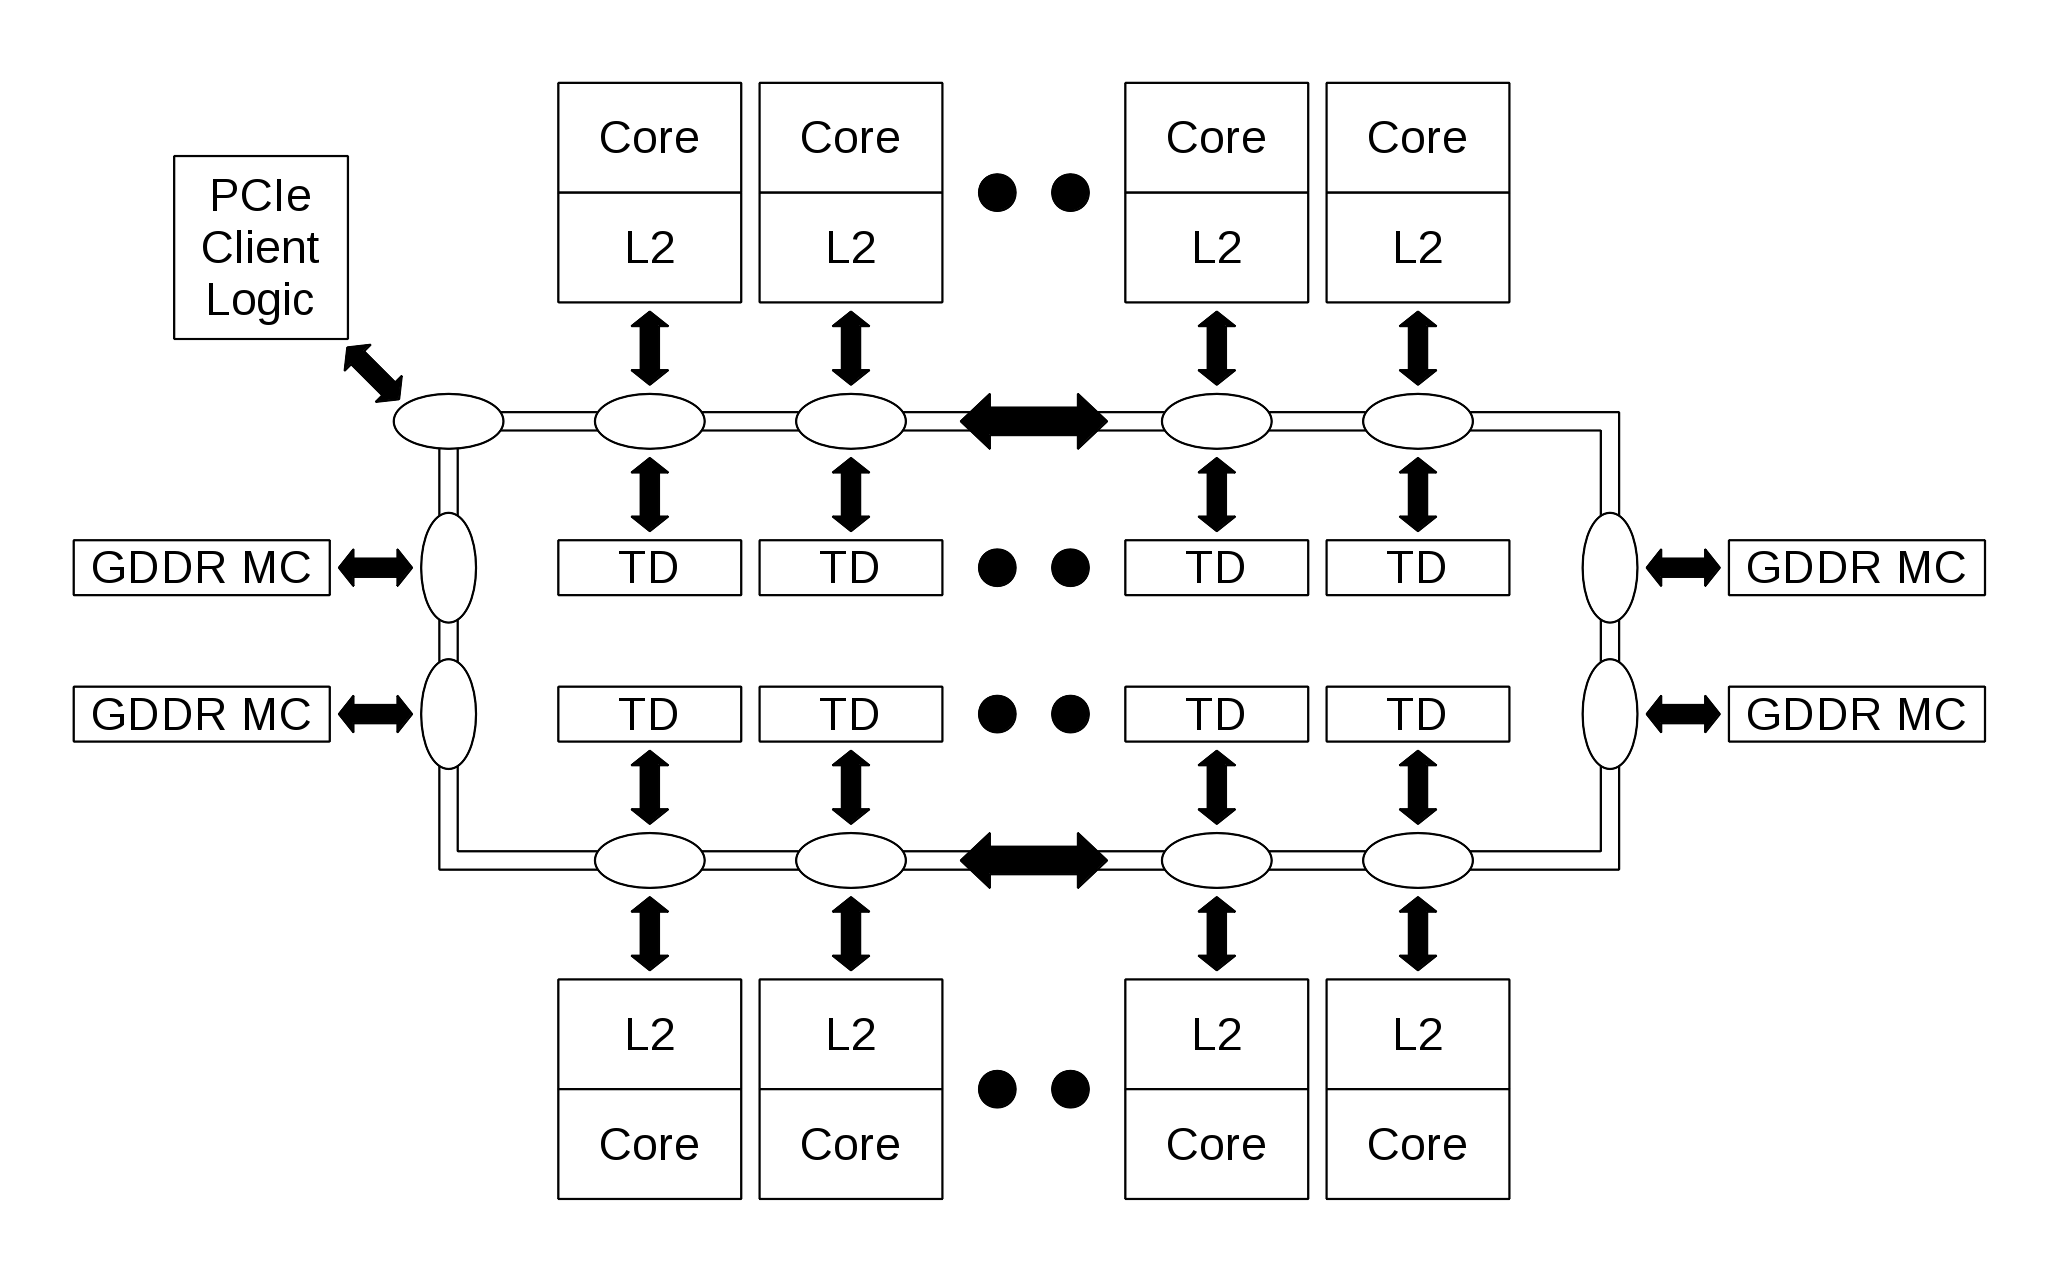
\includegraphics[width=\linewidth]{../diagrams/xeon_phi}
	\caption{Many Integrated Core (MIC) architecture of the Intel Xeon Phi\cite{overviewxeonandxeonphi}.}
	\label{Fig:xeonphi}
\end{figure}

The 5110P model used in this project contains 60 processing cores with a clock speed of 1052.63 MHz, each with four hardware threads. Cores communicate via a high-speed bi-directional ring-based on-die interconnect which minimises latency\cite{Jeffers13}. The card has 8GB of GDDR5 memory, and each core also contains 512 KB of L2 cache and 32 KB of L1 cache. L2 cache is kept coherent across all cores at the hardware level, using a Distributed Tag Directory (DTD) mechanism\cite{Jeffers13}. The maximum possible memory bandwidth is 320 GB/s\cite{intel5110p}. Each core also has a 512-bit SIMD Vector Processing Unit (VPU), which can process 16 single-precision or 8 double-precision elements per clock cycle\cite{Tousimojarad14}. The N-Queens benchmark described in Section \ref{Sec:nqueens} uses the vector units after the code is automatically vectorised at compile time.

\section{Parallel Performance} \label{Sec:parallelperformance}
A useful way to measure parallel performance is as performance gained relative to the serial version\cite{Blumofe95}. The execution time of a serial program is denoted \(T\textsubscript{serial}\). \(T\textsubscript{P}\) denotes the execution time of a parallel program running on \(P\) processors or threads. \(T\textsubscript{1}\) is therefore the execution time of a parallel program running a single thread. The efficiency of a parallel framework relative to a serial version of the same program can therefore be computed with the following formula\cite{Blumofe95}.

\begin{equation}
T\textsubscript{serial} / T\textsubscript{1}
\end{equation}

This definition has been widely used to determine the overhead introduced by parallel frameworks. Blumofe \textit{et al.}\cite{Blumofe95}, for example, used it to calculate the overhead introduced by MIT Cilk. Further, the parallel ``speedup" over the serial implementation achieved by a program when a certain number of processors are used can be computed with the following formula.

\begin{equation}
T\textsubscript{serial} / T\textsubscript{P}
\end{equation}

This is the measure by which the performance of benchmarks in this report are evaluated, since the goals of this project are not limited to evaluating the scaling of the benchmarks, but include evaluating the performance of the parallel frameworks themselves. The speedup reported is the performance of a given parallel benchmark making use of \(P\) threads relative to the serial implementation. Note that while \(P\) is the standard notation for the number of processors used in a benchmark, this report uses the notation \(t\), which is the \textit{parameter} passed to the benchmark programs at run-time to specify how many threads should be used.

\chapter{Benchmarks} \label{Sec:benchmarks}

In order to evaluate the relative performance of typical serial, OpenMP and Cilk Plus programs on the Intel Xeon and Xeon Phi devices, a suite of test programs was developed and their performance benchmarked on real hardware. This chapter describes the benchmarks written or modified for this project, including a traditional Fibonacci program, a parallel merge sort, a solution to the N-Queens puzzle and a modified version of the Unbalanced Tree Search (UTS) benchmark developed by Olivier and Prins\cite{Olivier09}. A literature survey is conducted for each benchmark, followed by a discussion of its suitability for this report. All benchmarks were implemented in C.

\section{Fibonacci} \label{Sec:fibonacci}

A benchmark that appears frequently in the literature is the `Fibonacci' program. The Fibonacci sequence is a sequence of integers presented by the Italian mathematician Fibonacci in the 13\textsuperscript{th} century. Starting with 0 and 1, each subsequent number \(n\) is the sum of the previous two numbers in the sequence. This gives the following sequence:
\begin{center}
\(0, 1, 1, 2, 3, 5, 8, 13, 21, 34, ...\)
\end{center}

The purpose of the Fibonacci program, denoted by the function \(fib(n)\), is to calculate the n\textsuperscript{th} number in this sequence. For example, \(fib(8) = 21\). This can be achieved by an almost literal translation of the mathematical definition of a given \(n\textsuperscript{th}\) integer to C code using recursive calls. A C function \verb!fib(int n)! is defined which contains two recursive calls to itself; one is passed \verb!n-1! as a parameter, the other is passed \verb!n-2!. The return value of the function is the sum of the values returned by these recursive calls. If the value of the parameter \verb!n! passed to the function is less than two, the function simply returns that value. It is this recursive behaviour that makes the Fibonacci program suitable for task-parallelism; if a new task is spawned for each of those calls, a task parallel framework should be able to schedule them for execution on one of the available threads. The same algorithm could be applied in a thread-based framework, but additional effort would need to be undertaken on the part of the programmer to implement a scheduling system that does not cause deadlock. Most serial implementations of the above algorithm will have only one parameter, \(n\), and return a single integer. However, task-based parallel implementations of the Fibonacci program, and of the other benchmarks discussed in this report, can include the number of threads the program may utilise as an additional parameter, denoted by \(t\).
\noindent
\begin{figure}
	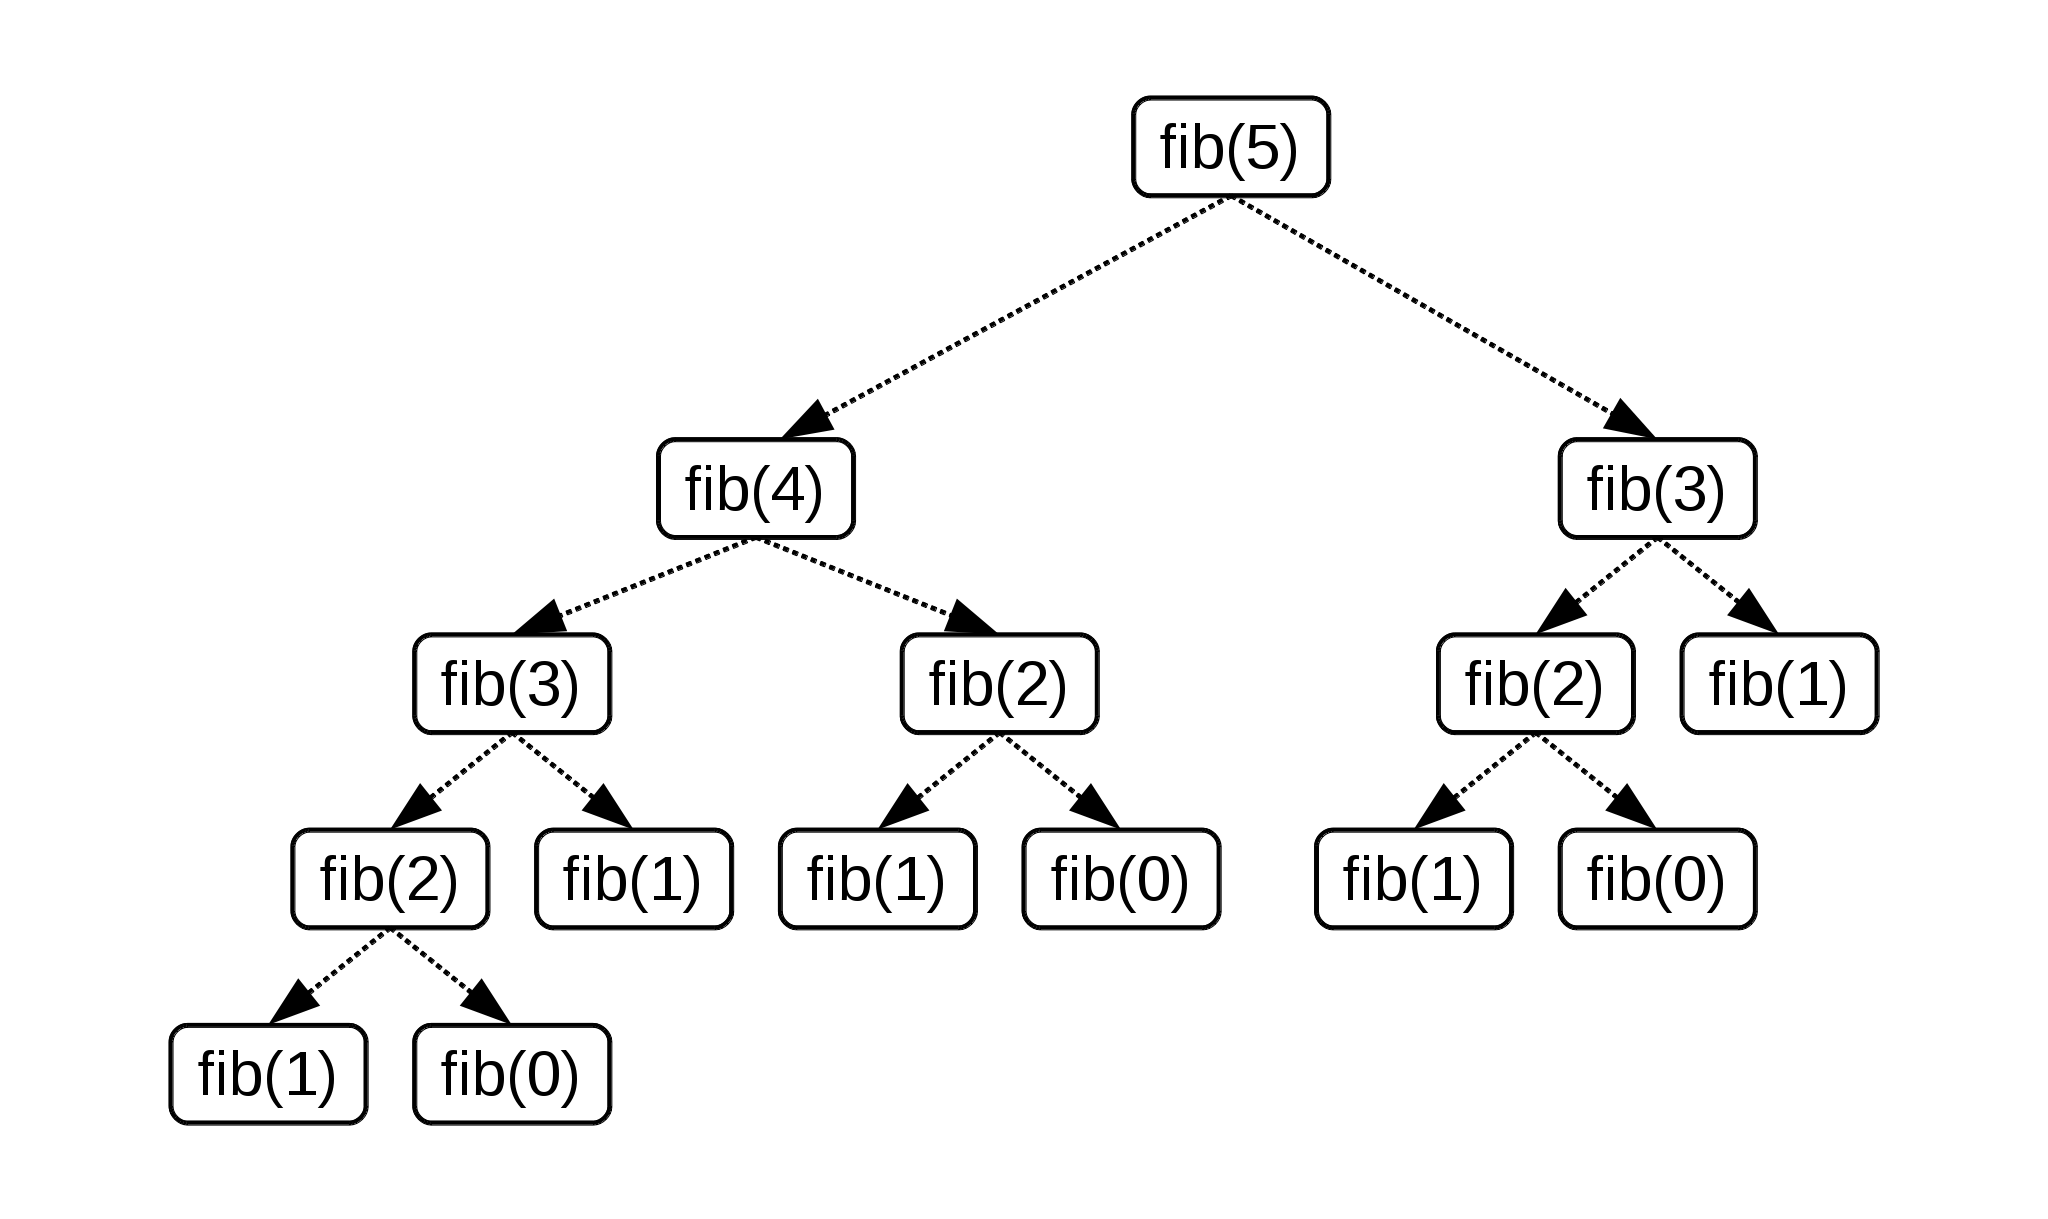
\includegraphics[width=\linewidth]{../diagrams/fib_tasks}
	\caption{Task spawning behaviour of the Fibonacci benchmark.}
	\label{Fig:fibtasks}
\end{figure}

The task-spawning behaviour of a parallel implementation of this algorithm is shown in Figure \ref{Fig:fibtasks}. In this example, the \verb!fib! function is passed the integer 5 when it is first called, resulting in two new tasks being spawned to execute the same function with the parameter values 3 and 4. Function calls that spawn new tasks are indicated with dotted arrows between nodes. When the new tasks are executed, they perform the same procedure recursively until a call is made to \verb!fib(2)! or \verb!fib(1)!. Note that all arrows in Figure \ref{Fig:fibtasks} are dotted, indicating that all calls to the \verb!fib! function, critically including those that only return a value, spawn new tasks. The fine granularity of this procedure is later shown to be a cause of inefficiency, and a promising variation on this algorithm that reduces the number of spawns is described in Section \ref{Sec:fibcutoff}.

Calculating the n\textsuperscript{th} number in the Fibonacci sequence was chosen as the first program to evaluate the performance of task parallelism on Intel Xeon and Xeon Phi processors because the algorithm described above, or variations on it, appears throughout the literature in performance evaluations of other hardware devices or configurations, as well as languages and libraries that provide support for concurrent programming.

Blumofe \textit{et al.}\cite{Blumofe95} included the Fibonacci program in their evaluation of the original MIT Cilk implementation. They state that its inclusion in their test suite is due to its short thread length, which makes it a good way to observe overhead introduced by parallelisation. The version used in their evaluation makes two recursive calls, as described above, but spawns a new task for only one of them. This variant reduces scheduling overhead, but is not included in this report due to time constraints. Blumofe \textit{et al.} observed near linear speedup in the calculation of the 33\textsuperscript{rd} number in the Fibonacci sequence; performance improved by 31.84 times on a 32-processor computer, and by 253.0 times on a 256-processor computer. 

In their evaluation of different strategies for load-balancing parallel applications, van Nieuwpoort \textit{et al.}\cite{Nieuwpoort01} observed a best-case speedup of only eight times with the two-spawn Fibonacci program on a cluster with 64 CPUs. In the worst case, caused by a particular scheduling strategy, execution time remained only half of the serial implementation. Olivier \textit{et al.}\cite{Olivier12}, who also evaluated scheduling strategies, but with OpenMP, typically observed a 12-16 times performance improvement of the parallel version over the serial equivalent when utilising 16 threads of two different machines. At 32 threads, the speedup varied greatly depending on the scheduling strategy used, ranging from 16 times in the worst case, to around 26 times in the best case.

In this report, the execution times of the Fibonacci benchmark are recorded for a range of input values. The complexity of the naive algorithm described here has a complexity of \(O(2^n)\), thus running the benchmark with the parameter \(n\) equal to each integer in the interval \([25, 35]\) gives a good idea of the performance trend. Execution of the Fibonacci benchmark after \(n=35\) quickly becomes prohibitively slow. Other, more efficient, algorithms have been devised that calculate the n\textsuperscript{th} number in the Fibonacci sequence. For example, Binet's formula reduces the complexity of the computation to constant time by exploiting the golden ratio. However, the purpose of including the naive algorithm in this report is not to demonstrate an efficient way of finding the \(n\textsuperscript{th}\) Fibonacci number, but to highlight differences between the performance characteristics of this and other benchmarks.

\subsection{Cut-off} \label{Sec:fibcutoff}

In order to reduce the number of new tasks spawned by the Fibonacci benchmark, an additional parameter can be introduced which controls the minimum value at which new tasks will be spawned by the \verb!fib! function. This `cut-off' parameter, \(c\), is passed to the \verb!main! function from the command line, and subsequently passed unchanged by each recursive call. Thus, setting the cut-off value to three will cause the \verb!fib! function, passed a value less than three as the \verb!n! parameter, to continue to make further calls to the \verb!fib! function, but without scheduling new tasks.
\noindent
\begin{figure}
	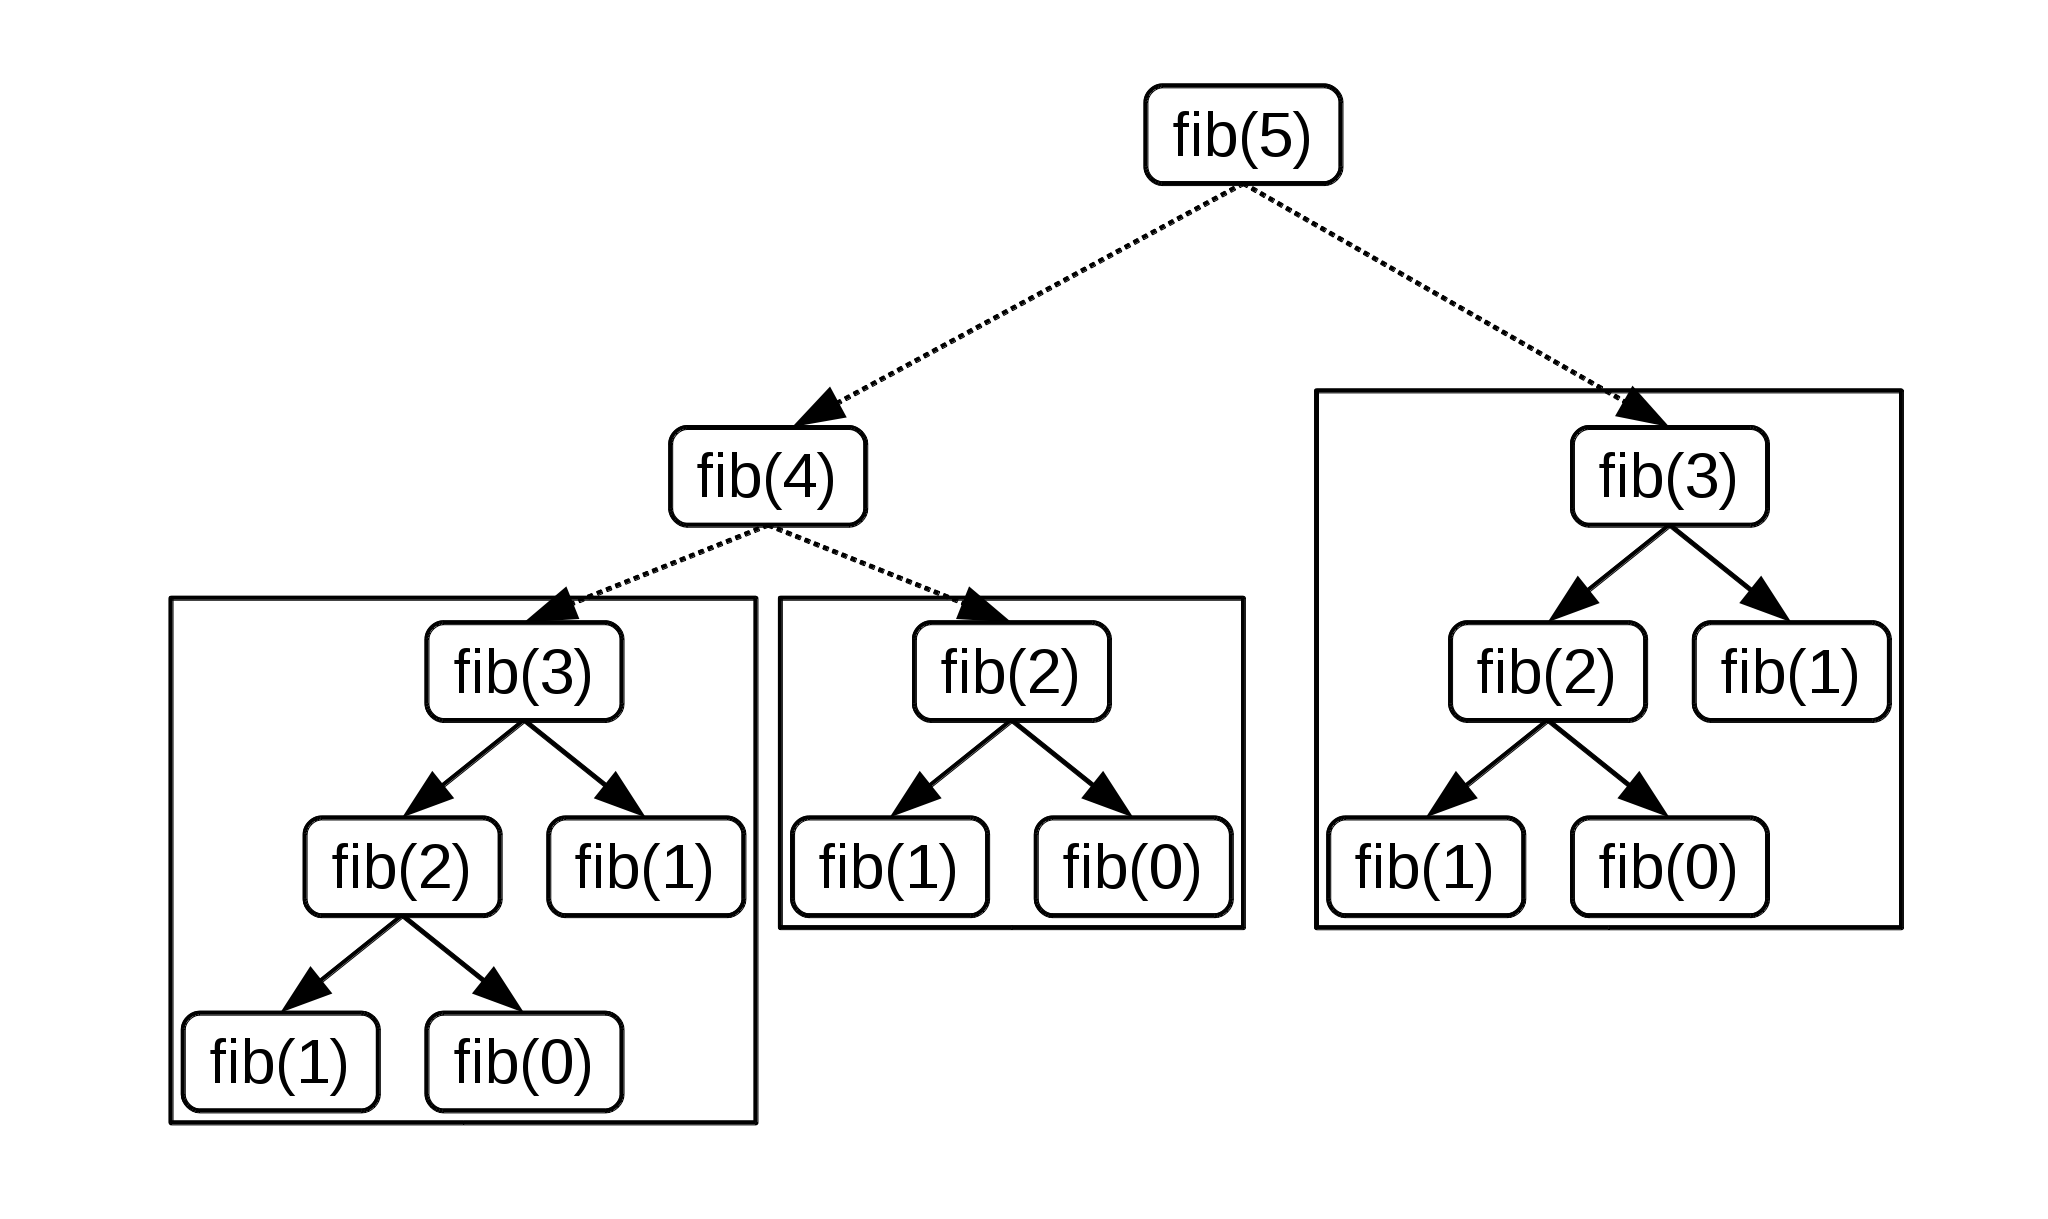
\includegraphics[width=\linewidth]{../diagrams/fib_cutoff_tasks}
	\caption{Task spawning behaviour of the Fibonacci benchmark with a cut-off value of three.}
	\label{Fig:fibcutofftasks}
\end{figure}

Figure \ref{Fig:fibcutofftasks} shows the effect of the cut-off algorithm on the previous example. Function calls that do not cause a new task to be scheduled are shown as solid arrows. For clarity, the work performed by a single task is encapsulated by a box. Note that for calls to the \verb!fib! function when the parameter \verb!n! is less than the cut-off value \(c=3\), no new tasks are spawned, and the lower levels of the task graph thus become serialised and the granularity of the algorithm becomes coarser.

This version of the Fibonacci program was adopted by Duran \textit{et al.}\cite{Duran09} into the Barcelona OpenMP Tasks Suite (BOTS). The authors state that the Fibonacci benchmark provides a useful example of very fine-grained parallelism, but that such fine granularity can be avoided by introducing the cut-off parameter. Subsequently, Podobas \textit{et al.}\cite{Podobas15} used the BOTS to evaluate different task-parallelism libraries, and found a 40 to 50 times speedup of the Fibonacci benchmark with \(n=47\) and \(c=15\) on a 64-core processor, dependent upon the framework used.

Tousimojarad and Vanderbauwhede\cite{Tousimojarad14} also used the Fibonacci benchmark with a cut-off value in their evaluation of the Cilk Plus, OpenMP and Intel Threading Building Blocks (TBB) task parallelism systems on Intel Xeon Phi. They found that speedup over the single-thread version achieved when using all 240 threads available on the Xeon Phi rose as the cut-off value was increased. They note that ``choosing a proper cutoff value is key to good performance''. In this report, a range of values for the cut-off parameter \(c\) are benchmarked with \(n=35\) in order to examine what level of cut-off is most appropriate for a program with this degree of parallelism.

\section{Merge Sort} \label{Sec:mergesort}

Another algorithm well-suited to task-based parallelisation is the merge sort. The merge sort algorithm is a method of creating a sorted list from a list of unsorted data. Given a one-dimensional array \verb!A! of size \(n\), a merge sort, denoted by the function \verb!msort(A)! produces a sorted array by recursively dividing the original array into two smaller arrays at each stage. When \(n=1\), no further division may occur, and \verb!A! is left unchanged. After both calls to \verb!msort! have returned, the function merges the two sub-arrays. In this project, the original array passed as the parameter in the first call to \verb!msort! contains \(n\) 32-bit integers. The complexity of the merge sort algorithm is known to be \(O(n log n)\), and an implementation using task parallelism can be produced by spawning a new task whenever \verb!msort! is called. Note that although the splitting of the array can easily be performed in parallel, the merge operation cannot so easily be applied to task parallelism. While it is possible to perform the merge operation in parallel, this has not been done in the implementations used in this project due to time constraints. As a result of this, the granularity of the program becomes more coarse because the number of extremely small tasks is limited.
\noindent
\begin{figure}
	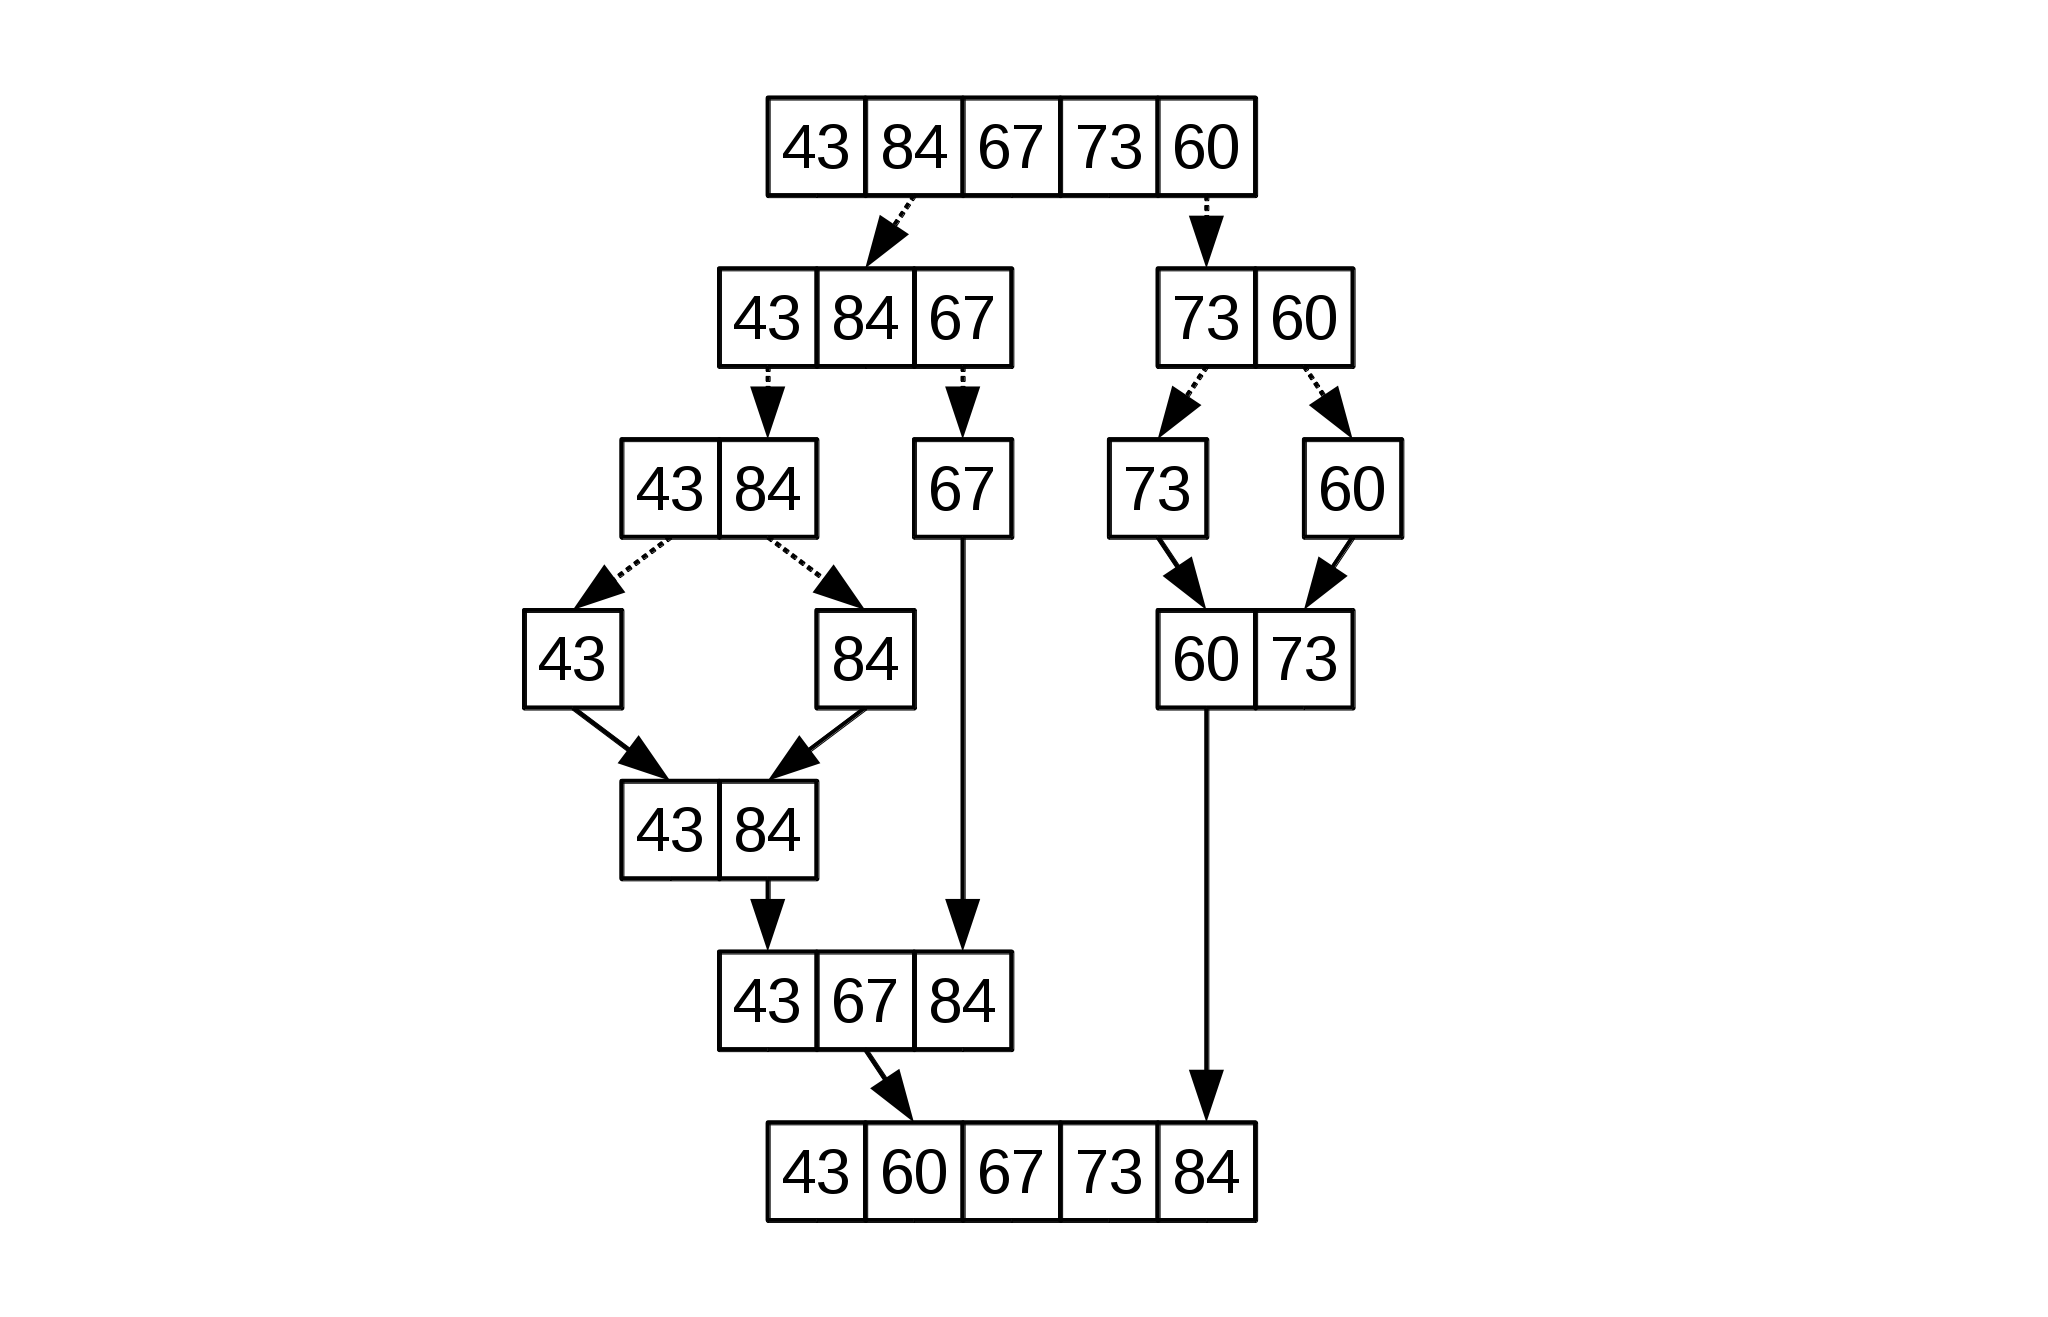
\includegraphics[width=\linewidth]{../diagrams/msort_tasks}
	\caption{Task spawning behaviour of the merge sort benchmark with five integers.}
	\label{Fig:msorttasks}
\end{figure}

Figure \ref{Fig:msorttasks} shows the task spawning behaviour of the parallel merge sort described above. The top level shows the original array, with size \(n=5\), and each subsequent level shows the split and merge operations that produce the sorted output. The split operations produce smaller arrays and are shown with dotted arrows, indicating that new tasks are scheduled. When the array cannot be subdivided further, sub-arrays are merged in a serial operation in the same task that spawned them. Each task therefore performs the merge operation only after any spawned tasks have returned. The joining of these tasks, as well as the merge operation, is shown in the diagram as solid arrows.

All implementations of the \verb!msort! function used in this project allocate all memory necessary for an array of size \(n\) of 32-bit integers when the program starts. This array is then filled with random integers between 0 and the maximum integer value defined by the compiler. The \verb!msort! function itself is not passed a sub-array directly, but a pointer to the location in the original array where the sub-array starts, as well as a size parameter indicating the length of the sub-array. Memory allocation is therefore not an additional operation performed by each task, because all memory management is handled by the \verb!main! function. For this report, the merge sort benchmark was executed with a range of input arrays of varying lengths. The smallest array used contained 100,000 elements, which rose in subsequent tests in increments of 100,000 up to three million.

Alternatives to this algorithm appear in the literature, including those utilising a cut-off value, and those that eliminate extremely fine-grain tasks by serialising the lower levels of the task graphs with other sorting algorithms. These alternatives are not explored in this project, because the purpose of this benchmark is to compare the performance on balanced and unbalanced programs performing otherwise the same operations. The merge sort was chosen for its ability to produce perfectly balanced task graphs if the size of the original array is a power of two. This is further described in Section \ref{Sec:powersoftwovariant}.

Ayguad\'{e} \textit{et al.}\cite{Ayguade09} used a variant of the merge sort in their description and initial performance analysis of OpenMP's tasking features. In their version, called \textit{multisort}, a serial quicksort is used ``when the array is too small". Conducting their tests on arrays which ranged in size between 32 million and 48 million integers, they observed an order of magnitude speedup over the serial version when using 32 CPUs. Notably, they also observed better speedup ratios when using fewer CPUs, indicating significant diminishing returns to applying more processors.

In their evaluation of different work scheduling strategies, Olivier \textit{et al.}\cite{Olivier12} used a parallel merge sort with a sequential quicksort and insertion sort at lower levels. Performing their benchmark on an array of 128 million integers, they observed almost four times speedup when using four threads of a four-socket Intel Nehalem computer, but a reduction in efficiency as the number of threads was increased. At 32 threads, each scheduling strategy tested achieved only around half of the theoretically possible performance improvement. It is important to note that because the lower levels of the task graph produced by the merge sort implemented for this project are not serialised, one may expect to observe even weaker scaling than presented by Olivier.

Tousimojarad and Vanderbauwhede\cite{Tousimojarad14} applied a cut-off value in the form of a fraction of the total work load. In their benchmark, a cut-off value of 2048 means that arrays produced by subdividing the original array that have a size less than one 2048\textsuperscript{th} of the original are sorted serially. In an array of 80 million integers, they tested a range of cut-off fractions between 16 and 2048 and like Olivier \textit{et al.} found that the merge sort did not scale well to many threads. However, they also observed that OpenMP and Cilk Plus achieved better performance than Intel TBB when the number of available threads was low, and that OpenMP and Intel TBB are preferred when the number of threads is increased. Utilising all 240 threads of the Xeon Phi, they observed a speedup of only around eight to ten times, attributing this to the high memory usage induced by the large size of the input vector.

The BOTS\cite{Duran09} version of the parallel merge sort was benchmarked by Podobas \textit{et al.}\cite{Podobas15}. In the BOTS, a parallel merge is used and a serial quicksort applied when the arrays are to small, to reduce task granularity. A speedup of between seven and eight times was observed when around ten to twenty threads were used, but additional threads caused performance to stagnate and even decline for some of the libraries being tested.

\subsection{Powers-of-two Variant} \label{Sec:powersoftwovariant}
One notable feature of Figure \ref{Fig:msorttasks} is that the task graph produced by the merge sort is unbalanced; some tasks do not spawn the same number of new tasks as others because the original array contains five elements. This feature can be eliminated by ensuring the length of input array is a power of two. When this condition is met and each array is recursively subdivided until it contains only one element, every task is balanced.
\noindent
\begin{figure}
	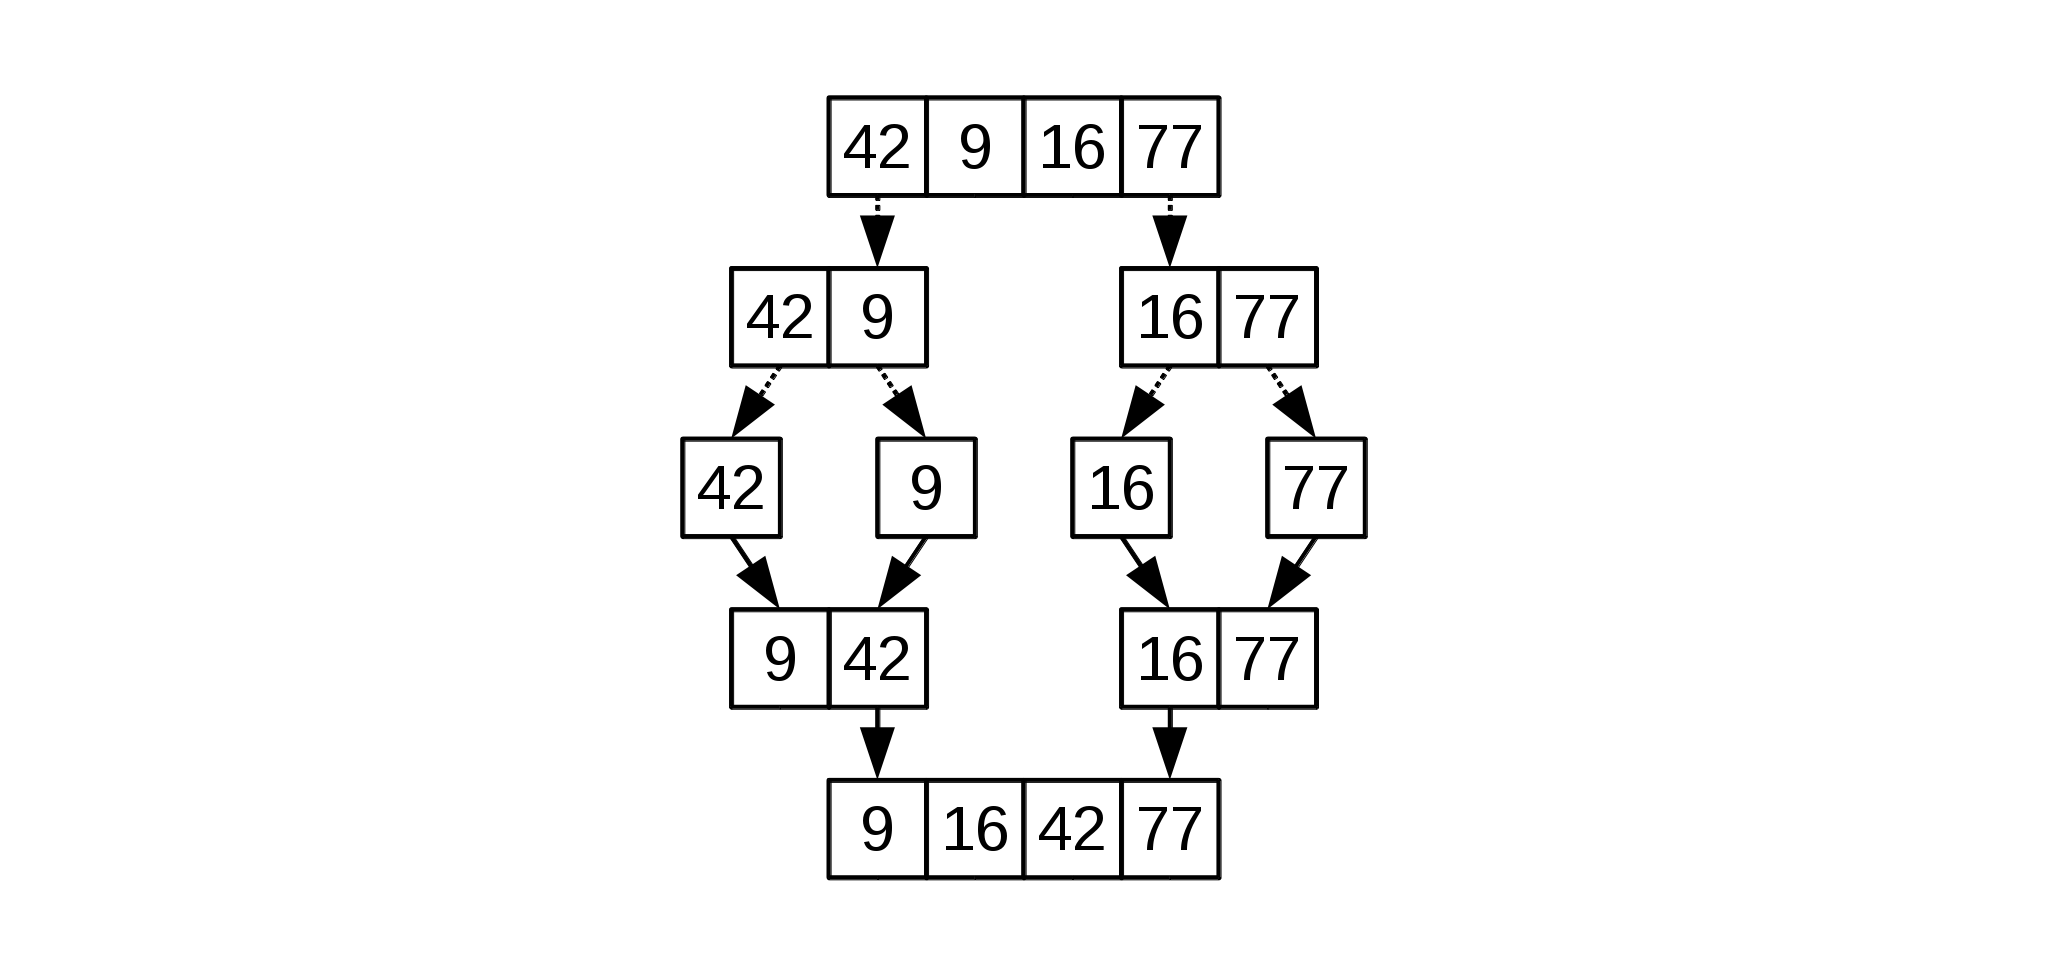
\includegraphics[width=\linewidth]{../diagrams/msort_powers_tasks}
	\caption{Task spawning behaviour of the merge sort benchmark with four integers.}
	\label{Fig:msortpowerstasks}
\end{figure}

Figure \ref{Fig:msortpowerstasks} shows the task graph of a merge sort performed on an array of length four. Because four is a power of two, it can be subdivided evenly until each sub-array contains one element, which will occur at the same level of the graph for all tasks. This presents the best-case scenario for task scheduling because it minimises the amount of work that may need to be moved between threads in order to maintain optimal thread utilisation. Included in the benchmarks is a series of tests called \verb!msort_powers! which have input vectors ranging from 2\textsuperscript{10} to 2\textsuperscript{22}. The results of these tests are compared with the results from the 
unbalanced merge sort in Section \ref{Sec:evalmsort}.

\section{N-Queens} \label{Sec:nqueens}

Of the benchmarks chosen for this project, one of the most frequent to appear in the task-parallelism literature is a program that solves the N-Queens problem. Given an \(n \times n\) chessboard, N-Queens attempts to place on it \(n\) queen pieces such that no queen may attack another. This means that no queen can share its row or column with another, but also that each diagonal only contains a single queen. The output of the program can be a list of the solutions found, but a common alternative is to instead output only the total number of solutions. Because the number of solutions is known for many values of \(n\), this can be a useful validation that the program is functioning as intended. Two example solutions to the N-Queens puzzle on \(8 \times 8\) chessboards are shown in Figure \ref{Fig:nqueenssolutions}. N-Queens was included in the benchmark suite because of the abundance of comparisons within the literature. It also has several interesting features, such as a task granularity that decreases with board size.
\noindent
\begin{figure}
	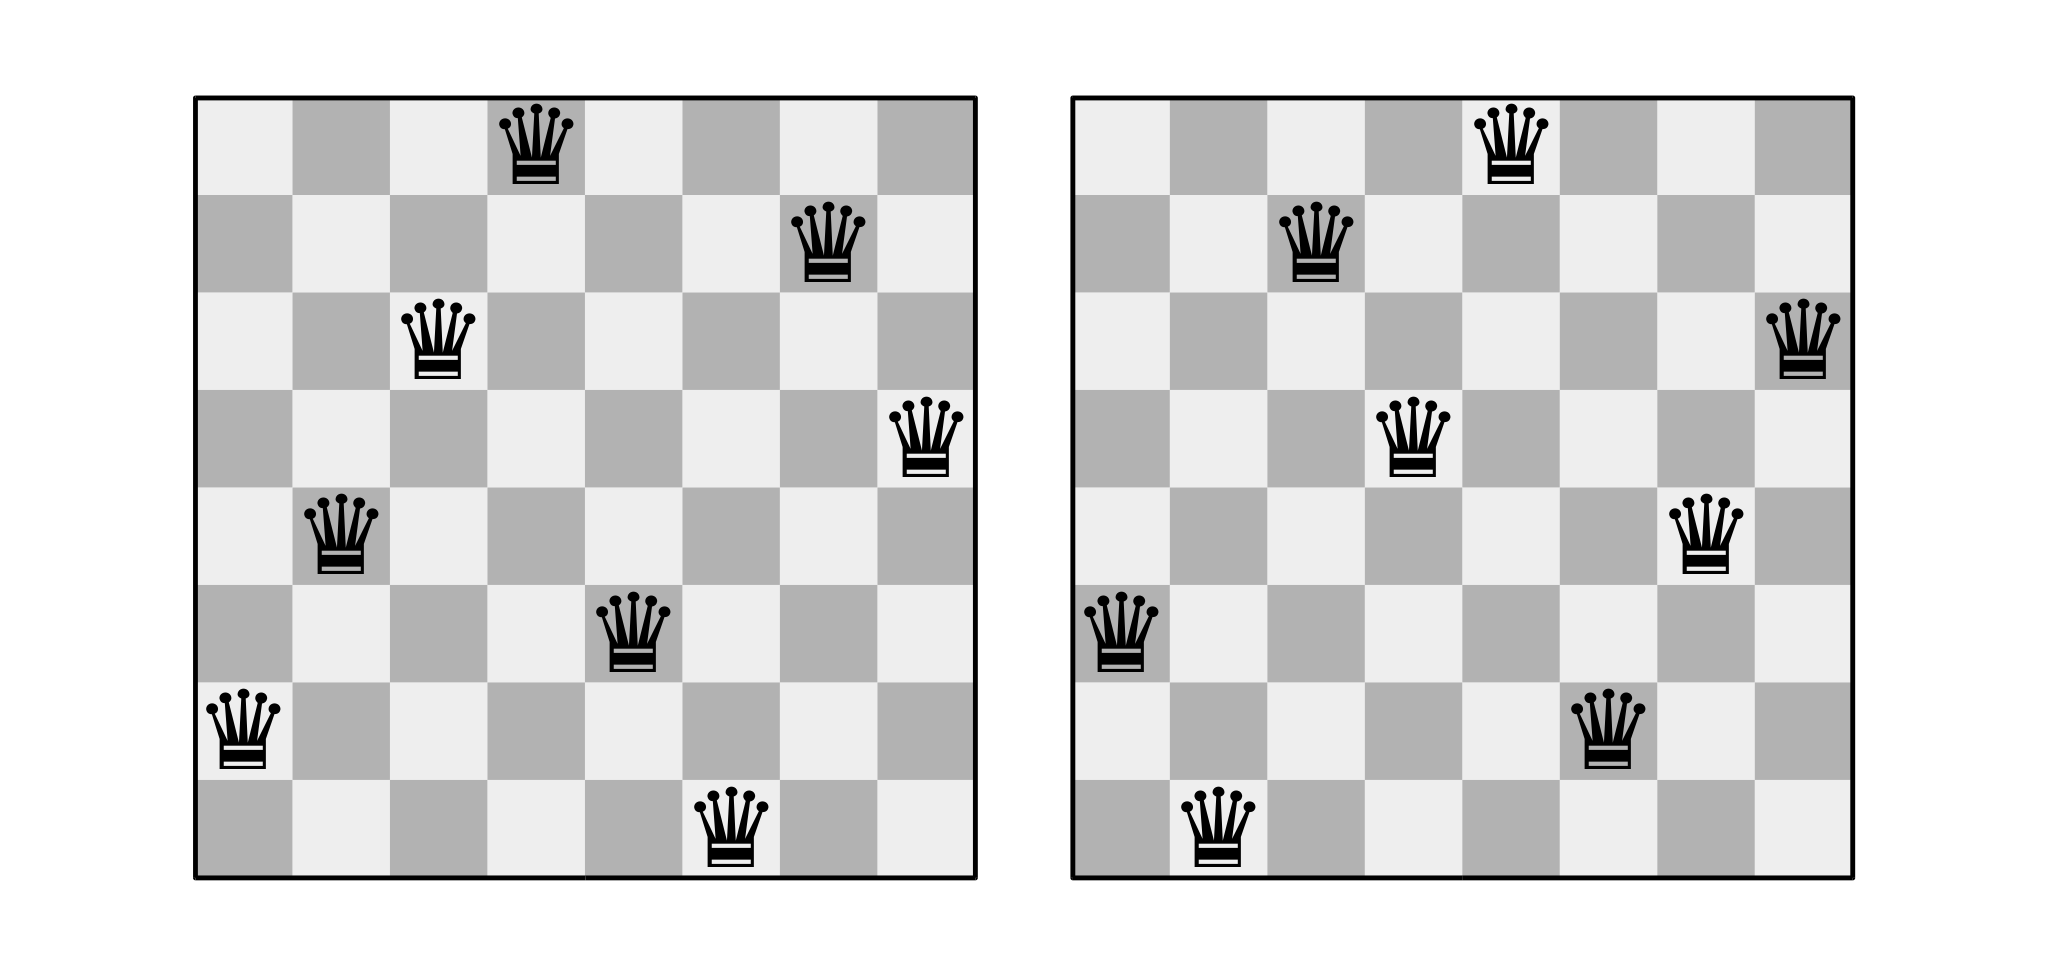
\includegraphics[width=\linewidth]{../diagrams/nqueens_solutions}
	\caption{Two valid solutions to the N-Queens problem on an 8 x 8 chessboard.}
	\label{Fig:nqueenssolutions}
\end{figure}

There are a number of different methods of solving the N-Queens problem, but those discussed here use a recursive back-tracking search algorithm similar to that proposed by Edsger Dijkstra in 1972\cite{Dahl72}. Dijkstra's approach is to start with an empty chessboard and proceed one queen at a time. When a queen can be placed without threatening another, it is placed on the board and the next queen is evaluated. If a queen is placed, but it threatens another, the algorithm removes the queen, reverting the board to the last known good state, and tries another position. When \(n\) queens have been placed successfully in this manner, the current board state must be a solution.
\noindent
\begin{figure}[t]
	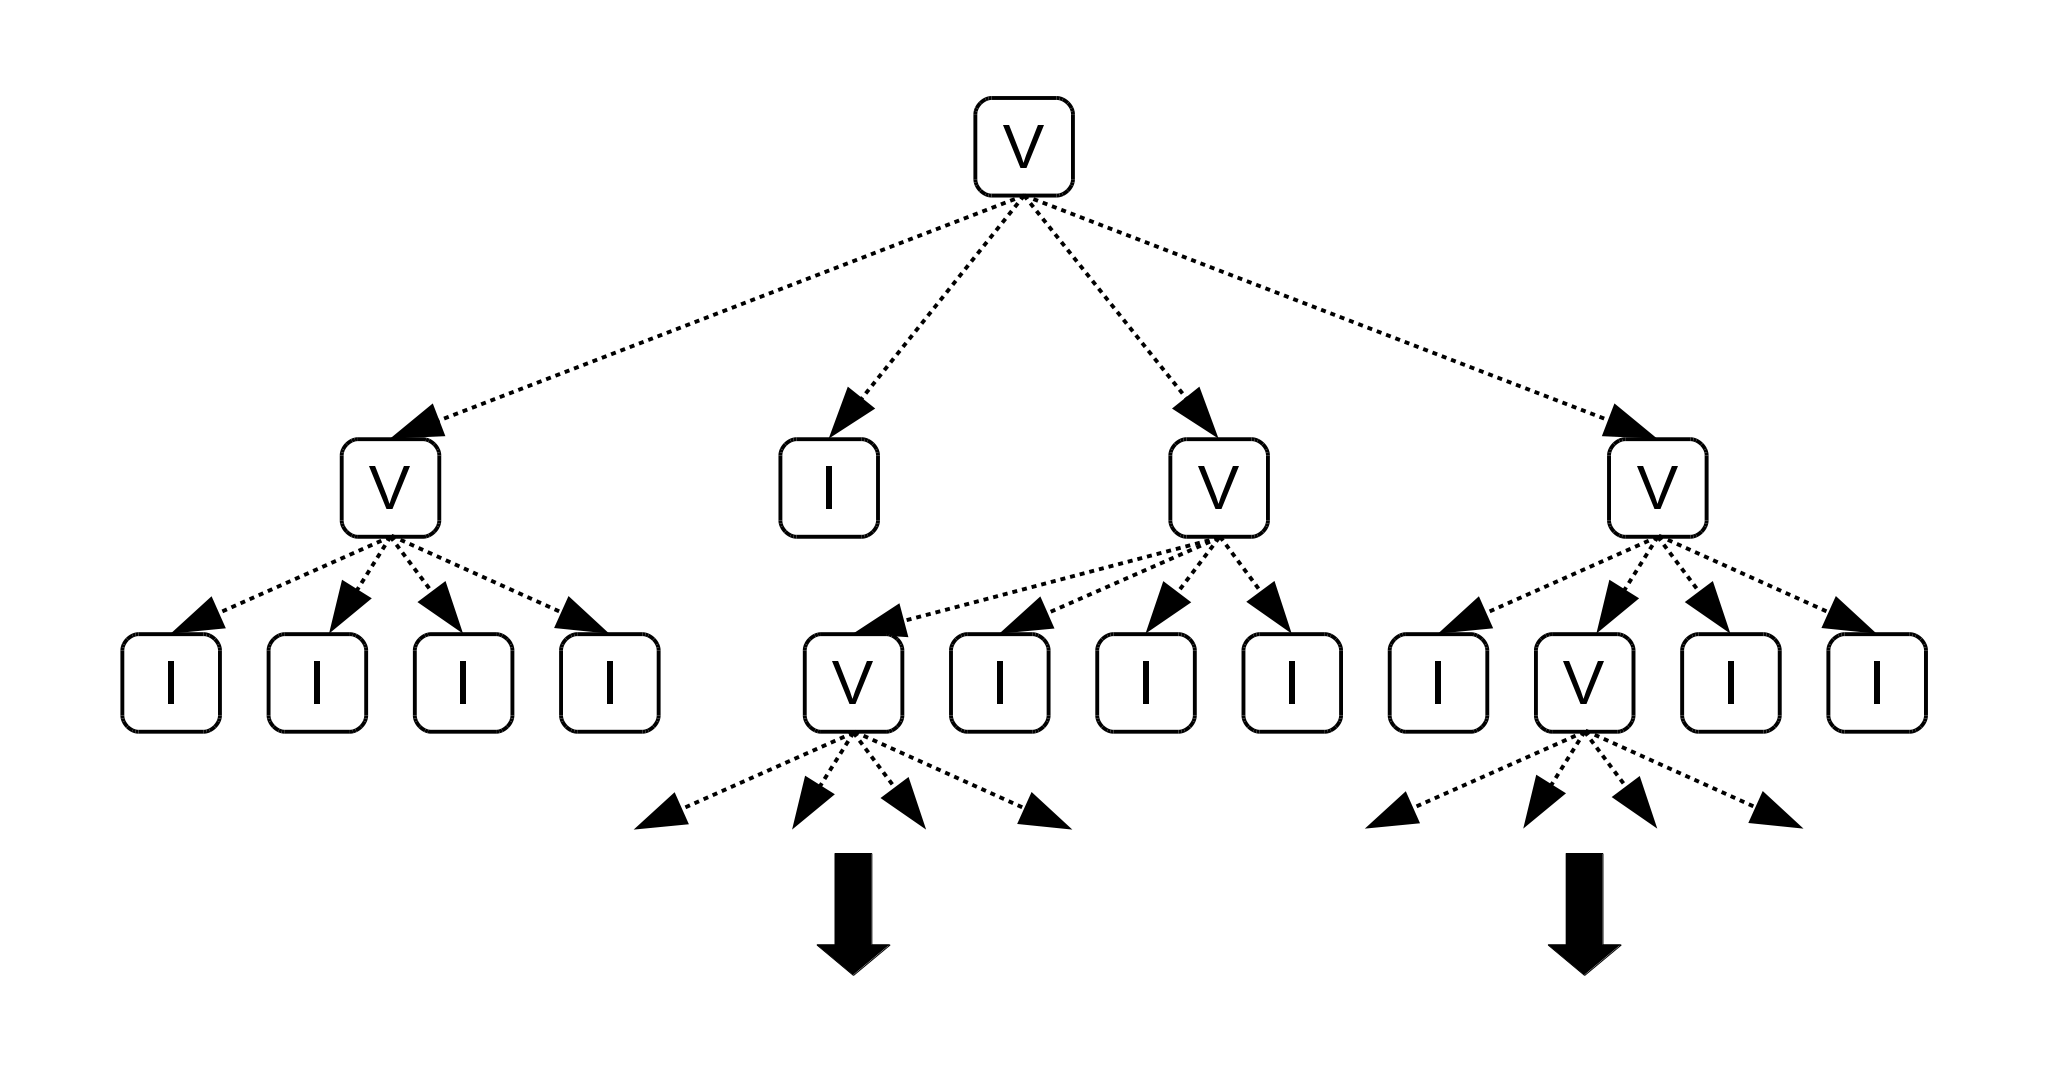
\includegraphics[width=\linewidth]{../diagrams/nqueens_tasks}
	\caption{Task spawning behaviour of the N-Queens backtracking search algorithm. `V' nodes represent board states that are valid. `I' nodes are invalid board states.}
	\label{Fig:nqueenstasks}
\end{figure}

Figure \ref{Fig:nqueenstasks} shows how tasks may be spawned by the N-Queens benchmark with a \(4 \times 4\) chessboard. Nodes labelled with a `V' represent valid board states, while nodes containing an `I' are invalid (i.e. two queens may attack each other). Note that valid states always spawn the same number of child tasks, except when the \(n\textsuperscript{th}\) level of the tree is reached, at which point any new `V' nodes would represent valid solutions. Invalid board states have no child nodes, because the back-tracking algorithm reverts the board state before any new tasks are spawned.

There are many ways to implement Dijkstra's algorithm. For example, one might model the board with a two dimensional array, and mark each element if it contains a queen. Another approach would be to exploit the binary nature of the squares, since their only two states are to be empty or contain a queen, and represent the board with binary an a standard type such as an integer or character. The algorithm implemented for this project is based on the approach published by Blair-Chappell and Stokes\cite{Blair12}, which exploits the fact that in a valid solution to the N-Queens puzzle, each row and column may only contain a single queen. They therefore model the board with a one dimensional array of size \(n\), where each element represents a row of the board. The integer contained within that element is the column which contains the queen on that row. As with the other benchmarks discussed in this report, the purpose of including this algorithm is not to demonstrate an efficient way of solving the N-Queens puzzle, but to highlight particular aspects of how it may be efficiently parallelised.

One feature that makes the N-Queens program different from the benchmarks discussed so far is that it uses for-loops. For each row of the board, a queen must be placed. And for each column in a given row, all squares must be considered to determine if a queen could be placed there to produce a solution. But the N-Queens problem also introduces a difficulty not seen in either the Fibonacci or merge sort benchmarks. In the serial version, the number of solutions found on branches leading from the for-loops must be summed serially. In a parallel version, this could lead to a race condition if care is not taken to either use an atomic count or serial sum. For easy comparison between the serial version and the task-parallelism libraries, an array of solutions counts is used with each for-loop. Each iteration \verb!i! of the loop stores its returned value in element \verb!i! of the array, and a serial sum function finds the total number of solutions found. In the Cilk Plus implementation, the standard C for-loops can be replaced with \verb!cilk_for!, discussed in Section \ref{Sec:usingcilkplus}. During development an attempt was made to write an OpenMP version using standard nested parallel loop pragmas, but this resulted in the program failing to terminate because it would wait for threads to be freed. The version using OpenMP tasks instead spawns a new task for each iteration of the for-loop, then synchronises the tasks before summing the results. A race condition may also occur if multiple threads attempt to place queens on the same board. This is avoided by passing a copy of the current board state to each newly spawned task, which is then deleted when the function returns. These two features cause the granularity of the program to decrease with \(n\).

Another feature of N-Queens not explored in the other benchmarks is its use of the vector units available on the hardware. With auto-vectorisation enabled, the Intel C++ Compiler (icc) is able to vectorise the \verb!sumArray! function, which sums the elements of an array passed as an argument. Using the \verb!-vec-report! option during compilation shows that icc estimates the potential speedup of this optimisation to be around 2.8 times. In evaluating the performance of N-Queens, two versions were produced: one with auto-vectorisation enabled during compilation, and one with auto-vectorisation disabled during compilation.

The N-Queens program was used in an evaluation of MIT Cilk by Blumofe \textit{et al.}\cite{Blumofe95}, who serialised the bottom seven levels of their implementation. This variant was also benchmarked for this project, and is described in Section \ref{Sec:nqueenscutoff}. As in their Fibonacci benchmark, Blumofe \textit{et al.} observed an almost linear speedup with 256 threads. Nieupoort \textit{et al.}\cite{Nieuwpoort01} have also used the N-Queens benchmark, but do not state whether or not they used a cut-off. They observed a wide range of performance variations depending upon the strategy used to schedule new tasks; speedup of almost 60 times could be achieved on a 64 CPU cluster, but this fell to less than 10 times for some trials. Rehr and Vinter \cite{Vinter08} used their N-Queens program to place 18-20 queens in an evaluation of the memory performance of the Cell-BE processor, finding that manual vectorisation allowed simultaneous searches of four branches of the tree. Ayguad\'{e} \textit{et al.}\cite{Ayguade09} compared implementations using nested OpenMP parallel loops, OpenMP tasks and Cilk. They found that nested OpenMP loops were the least performant approach, while OpenMP tasks and Cilk achieved similar speedup. The performance of all implementations stagnated when 20 CPUs were used with \(n=12\), \(n=13\) and \(n=14\). In Section \ref{Sec:evalnqueens}, values of \(n\) between 2 and 13 are used to reveal how thread utilisation and load balance changes with greater work-loads.

\subsection{Cut-off} \label{Sec:nqueenscutoff}

A variant of N-Queens with a cut-off parameter \(c\) was also developed and is included in the benchmark suite. Like the Fibonacci cut-off benchmark, this is used to identify the effectiveness of this approach when applied to different algorithms. The cut-off parameter in N-Queens lies between 0 and \(n\), and represents the number of rows from the beginning that may spawn new tasks. For example, setting \(c=4\) on an \(8 \times 8\) chessboard would cause only half of the rows to spawn new tasks when the for-loop is encountered. In Section \ref{Sec:evalnqueenscutoff}, the size of the chessboard is held at \(13 \times 13\), and the cut-off parameter \(c\) incremented from 0 to 13. The performance is measured at each step. Note that \(c=0\) is equivalent to a serial version of N-Queens.

\section{Unbalanced Tree Search} \label{Sec:unbalancedtreesearch}

Because a key aspect of achieving optimum parallel performance is efficient load-balancing, a benchmark that tests the load-balancing capabilities of Cilk Plus and OpenMP was included. The Unbalanced Tree Search (UTS) is an artificial benchmark developed by Olivier and Prins\cite{Olivier09} which was specifically designed to stress the scheduling and load-balancing capabilities of a parallel system. The UTS benchmark generates a tree in which each node has an unpredictable number of children, which Olivier and Prins claim presents the system with a highly unbalanced task graph. The depth, shape and granularity of the tree generated can be affected at runtime by changing parameters passed via the command line.
\noindent
\begin{figure}
	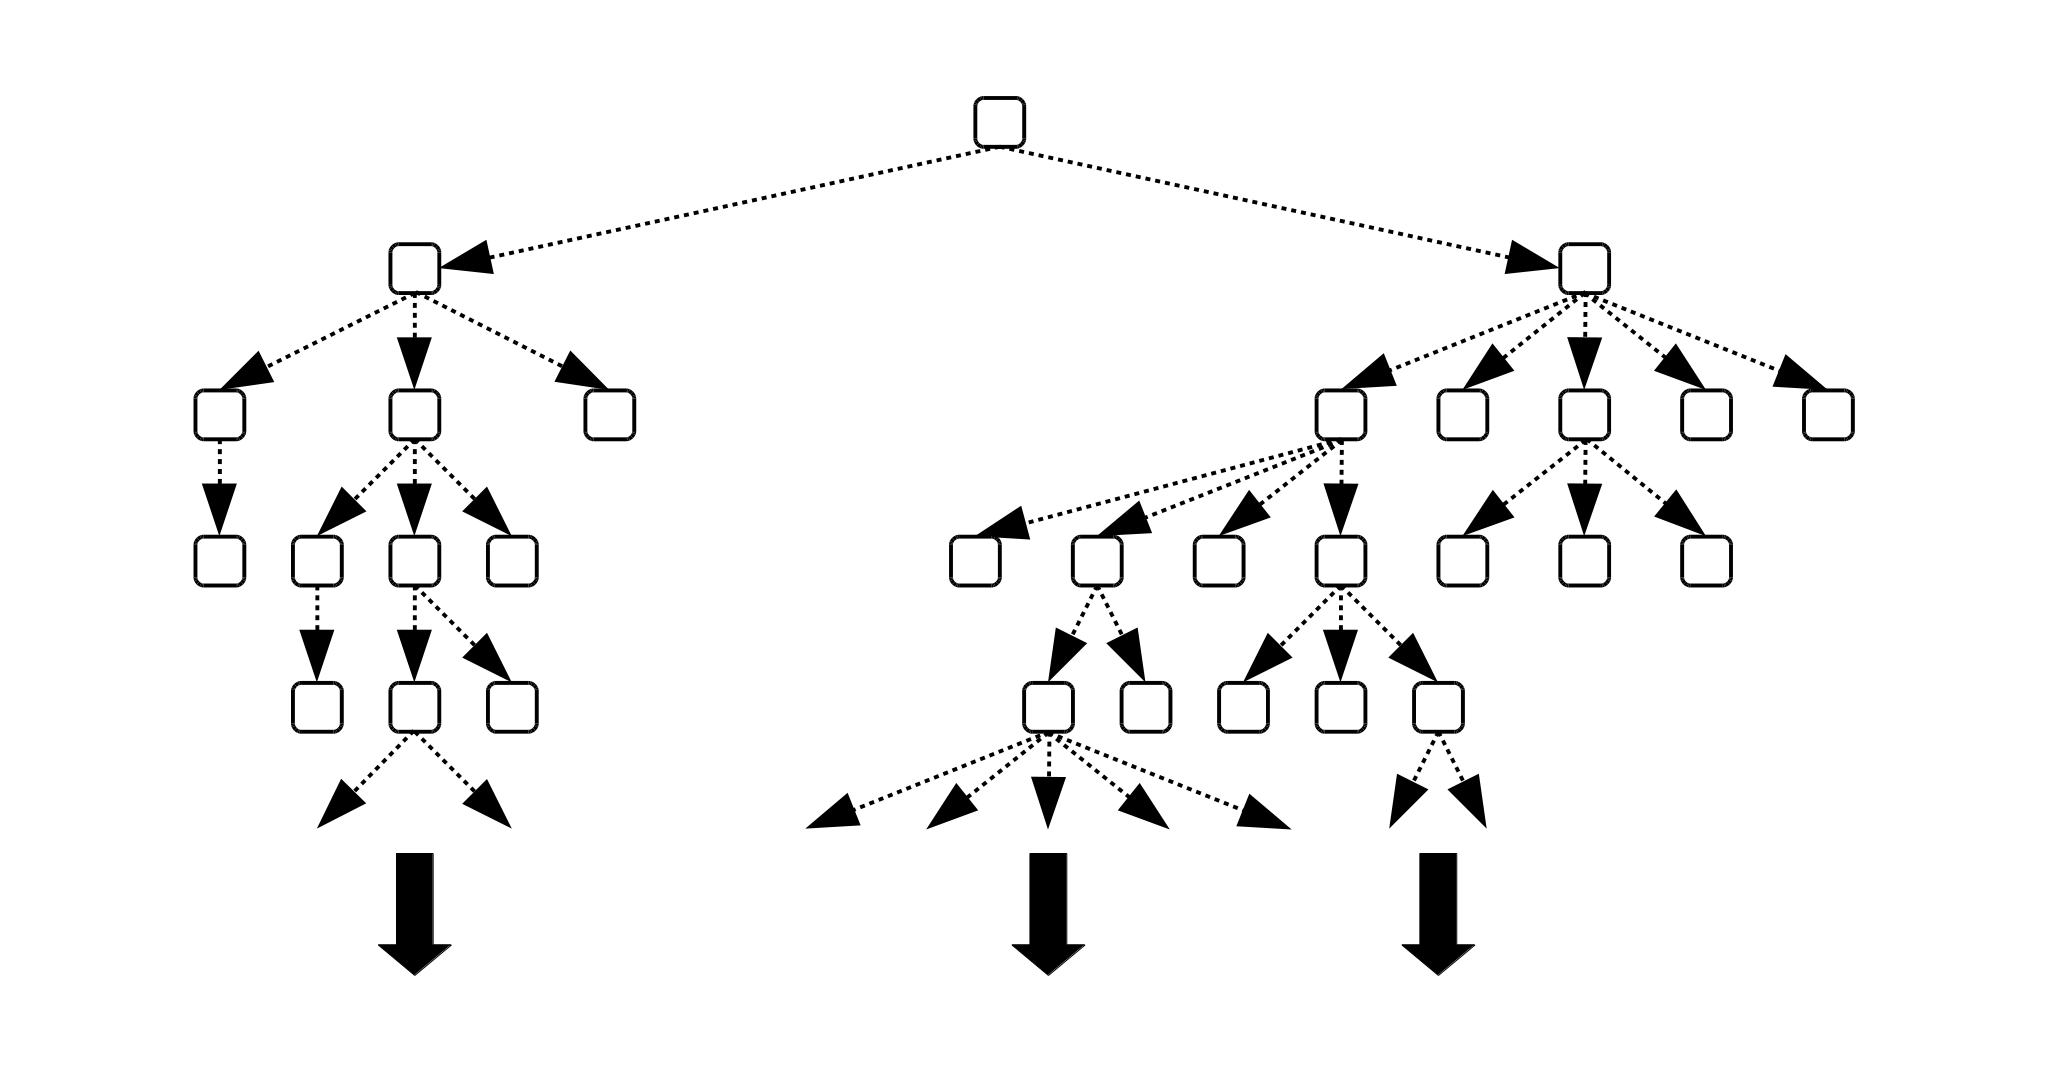
\includegraphics[width=\linewidth]{../diagrams/uts_tasks}
	\caption{Task spawning behaviour of a tree generated by the UTS benchmark.}
	\label{Fig:utstasks}
\end{figure}

Figure \ref{Fig:utstasks} shows the possible task spawning behaviour of a tree generated by the UTS benchmark. When a new child node is spawned, a new task is created to perform the generation of its children, shown as dotted arrows. Though apparently random, the trees generated by the UTS benchmark are actually deterministic. To avoid synchronisation across multiple threads attempting to update a single random number generator, Olivier and Prins use the SHA-1 cryptographic hash function to produce pseudo-random numbers based on the `description', a twenty character string, assigned to the spawning node. Nodes being generated on different threads, therefore, do not produce the same number of children and the tree remains unbalanced. If the same seed value is used to initialise the root node, the hash function should produce the same tree regardless of the order in which tasks are scheduled. Another advantage of this approach is that is provides manual control over the granularity of the tasks. By executing the hash function repeatedly on a single node's description, the time spent spawning each new child is raised and the task granularity decreases. This is controlled with the granularity parameter \(g\).

Olivier and Prins' original UTS implementation is available as open source software\cite{UtsSite}, which includes a set of pre-defined parameters and the results expected from generating a tree with those parameters, such as the total number of nodes generated. This was later modified by Jens Breitbart\cite{UtsSimpleSite}, who simplified it while guaranteeing that it still produced the same trees. This version was further modified for this project. A new command line option, \verb!-w!, was added to control the number of threads that the program may utilise, and a count of the total nodes generated was included to confirm that the results matched the value expected from Olivier and Prins' original tree list. The program was then converted to C and Cilk Plus and OpenMP commands were added to implement concurrency. For Cilk Plus, this involved use of the \verb!cilk_for! command in a similar manner as it is used in the N-Queens benchmark. Likewise, the OpenMP implementation uses the same technique as N-Queens, in which tasks are spawned by a standard C for-loop, and joined immediately after.

In this project, a pre-defined set of parameters from Olivier and Prins' list is selected, and the speedup achieved by applying more threads to the Cilk Plus and OpenMP versions is recorded. Because the UTS benchmark differs from others described in this chapter in that is has no \(n\) parameter, the \(g\) parameter, which controls the granularity of tasks, is incremented between one and ten. In other words, the description of each new child is generated by between one and ten iterations of the SHA-1 hash function.

When generating a tree with 4.1 million nodes on a system containing eight dual-core processors, Olivier and Prins\cite{Olivier09} found that parallelisation with Cilk provided significant performance benefits, and that these gains continued as more threads were made available. At 16 threads, Cilk provided a speedup over the serial benchmark of ten times. In another paper, the same authors\cite{Olivier10} tested the tasking capabilities of OpenMP 3.0, Cilk++ and Intel TBB, and found that all provided speed improvements of around eight times on a 16-core system, but that Cilk++ outperformed the alternatives. Podobas\cite{Podobas15} \textit{et al.} used the UTS benchmark to conduct a survey of the same libraries on a 64-core processor and found that all except Intel TBB actually slowed down the execution of the benchmark. Interestingly, they found that a new system, Wool, achieved almost linear speedup.

\chapter{Evaluation} \label{Sec:evaluation}

This chapter details the results obtained from running the benchmarks described in Chapter \ref{Sec:benchmarks}. For each benchmark, performance features that appear in the data are described and explained with reference to hardware factors and the existing literature.

\section{Benchmarking Process} \label{Sec:benchmarkingprocess}

This section describes the process and methodology used to perform the benchmarks outlined in Chapter \ref{Sec:benchmarks}. Issues including timing on different hardware are discussed, followed by a description and justification of the automated process that was developed to manage the many benchmarks conducted for this project.

\subsection{Timing Functions} \label{Sec:timingfunctions}
An important aspect of investigating the performance of the benchmarks in this project is accurate measurement of execution time. The high clock-rate of modern processors makes the timing of small programs difficult, but the Xeon and Xeon Phi processors have features that allow the use of timing techniques that yield measurements with nanosecond accuracy.

All Intel x86 processors since the Pentium feature a 64-bit register called the time-stamp counter. Although the Intel Xeon Phi uses the MIC architecture, its design also includes this counter This is accessible through the \verb!RDTSC! assembly instruction and gives an accurate count of the number of the cycles that have occurred since the last reset\cite{Rdtsc}. Because the \verb!RDTSC! instruction returns the number of cycles since the last reset and not the time elapsed, the count must be converted to time with the following formula\cite{Rdtsc}.

\begin{equation}
seconds = cycles / frequency
\end{equation}

While this would appear to give an accurate time measurement, Intel's documentation notes that the instruction is subject to out-of-order execution, meaning the \verb!RDTSC! instruction might not return the time-stamp counter at the exact point that was intended when the code was written\cite{Rdtsc}. The impact of this characteristic on the timing of programs executing many instructions is unlikely to be significant, but the exact location of the \verb!RDTSC! instruction in the code can at least be determined by requesting assembly output from the compiler. This can be used to confirm that the timing function is capturing the main part of a benchmark, even if the order of execution cannot be guaranteed.

Additionally, Microsoft discourages the direct use of the \verb!RDTSC! instruction because multi-core processors may switch a thread to run on a different core without guaranteeing that the cycle counter is synchronised during migration\cite{GameTiming}. Microsoft also warns that automated power management on modern motherboards may include varying the frequency of the CPU. Some models of Xeon and Xeon Phi, including those used in this project, eliminate the latter problem by explicitly synchronising the time-stamp counter across all cores\cite{Jeffers13}. The clock rates of the Xeon and Xeon Phi are also fixed, meaning that the number of CPU cycles that have passed since the last sample can be converted into real time without accounting for power management.

To avoid writing the timing functions in assembly directly, a native Unix function for retrieving time was wrapped into C functions for easy and consistent time measurements. The \verb!clock_gettime! Unix function can be instructed to use one of several available system clocks. Jeffers and Reinders\cite{Jeffers13} timed the clocks available in the Xeon Phi and concluded that the \verb!CLOCK_REALTIME! clock is accurate to within 200 nanoseconds. This is the clock used in all of the trials conducted for this project. This Unix function was wrapped into two simple functions: \verb!startTimer!, placed immediately before the instructions to be timed, and \verb!stopTimer!, placed immediately after. All the benchmarks include these functions via the \verb!timer.h! header, available in Appendix \ref{App:timerh}.

A problem with these timing functions arose during development. Because optimisations were enabled via the \verb!-O2! switch on the Intel compiler, it was discovered that the compiler was in fact optimising out the very functions that were intended to be timed unless the output produced by those functions (such as the \(n\textsuperscript{th}\) Fibonacci number) was used in some way in the rest of the program. The simplest way to use the output turned out to be to store it in a variable and output it via the \verb!printf! function along with other relevant information such as input parameters and execution time. This proved to be unexpectedly useful because a race condition within the UTS benchmark was discovered accidentally when the output did not match the expected value in some cases.

\subsection{Preparing and Running Benchmarks} \label{Sec:prepandrunbench}
During the development of the benchmarks, it became necessary to perform test compilations with the Intel compiler available on the host machine. These frequent tests highlighted compilations errors, as well as warnings that may indicate dangerous behaviour, such as implicit type casts. The time needed to setup these compilations and run the resulting binaries on both the host machine itself and the MIC architecture eventually became a large enough time investment that it was worth finding an automated alternative. This allowed faster iteration on the design of the benchmarks and more frequent error checks. This section describes the process of preparing and executing benchmarks on the Xeon Phi and host machine, and the workflow that was developed to send and receive data to and from these devices with as little repetition of manual tasks as possible.

Executing programs on the Xeon Phi remotely is a multistage process, involving copy operations both too and from the Xeon Phi and host machine. Because physical access to the host machine was not available, it was necessary to use remote access via the SSH protocol. Typically, this was done from the Department of Computer Science Linux Lab, but access to the host machine could also be gained off-campus using the same method. In order to execute programs on the Xeon Phi, they must be compiled for the MIC architecture by the Intel C++ Compiler (icc) with the \verb!-mmic! flag. Because the Xeon Phi runs only a minimal distribution of Linux, and does not have the Intel compiler installed on the device itself, programs must be compiled on the Intel Xeon host machine, and the resulting binaries copied to an available MIC device with the \verb!scp! (secure copy) Linux command. The \verb!mic0! device was used for all of the Xeon Phi benchmarks described in this report. Copying source files to the host machine can also be done remotely. Thus, a typical session using the manual approach might look as follows:
\hfill\\

\begin{center}
	\begin{tabular}{| l | l | }
	\hline
	{\bf Action} & {\bf Command} \\ \hline
	Copy source code to host & \verb!scp <source> <host>! \\
	Connect to host machine & \verb!ssh <host>! \\
	Compile source for host & \verb!icc <source>! \\
	Compile source for MIC & \verb!icc <source> -mmic! \\
	Execute host benchmark & \verb!./<binary>! \\
	Copy binary to Xeon Phi & \verb!scp <binary> mic0:~! \\
	Connect to Xeon Phi & \verb!ssh mic0! \\
	Execute MIC benchmark & \verb!./<binary>! \\ \hline
	\end{tabular}
\end{center}
\hfill\\
As the number of source files increased and the variety of options used for the benchmarks expanded, it became worthwhile to automate large parts of the process with bash scripts. Bash is a language built into Linux which provides useful functionality such as automated execution of commands, for-loops, functional abstraction and environment management (such as the setting of environment variables). For example, a script was written to automatically copy large numbers of files from a local machine to the host machine without having to repeatedly type its IP address. Another script was used to connect to the host machine, and then to \verb!mic0!, automatically copying library files from obscure directories which the Xeon Phi needed to execute OpenMP and Cilk Plus code. A list of the most useful scripts developed for this project is shown below:
\hfill\\

\begin {center}
	\begin{tabular}{ | l | p{10cm} | }
	\hline
	{\bf Script} & {\bf Description} \\ \hline
	\verb!push! & Copy all files in the `host' directory to the host machine. \\ 
	\verb!sshh! & SSH to the host machine and move to the appropriate working directory. \\
	\verb!build! & Compile all benchmarks. \\
	\verb!cpm! & Copy specified files to mic0. \\
	\verb!sshm! & SSH to mic0 and copy the necessary library files to a temporary folder. \\
	\verb!run! & Set up the necessary environment variables and execute the specified binaries. \\
	\verb!benchh! & Run a suite of benchmarks on the host machine with different options; automated with functions and for-loops. \\
	\verb!benchm! & Same as benchh, but for the MIC architecture. \\ \hline
	\end{tabular}
\end{center}
\hfill\\
The most important scripts are included in Appendix \ref{App:scripts}. The time needed to execute all the benchmarks in the \verb!benchm! script on the Xeon Phi was over twenty hours, so they were often executed over night. Because this proved impractical when making adjustments to the programs during development, several methods of reducing the benchmarking time were used. Often, it was reasonable to limit trials to a subset of the total benchmarks in order to test particular aspects of the process or programs. For example, when a race condition was detected within the UTS benchmark, all preceding tests were skipped by commenting out their function calls in the bench script. Another approach, used to identify the cause of unexpected results from the merge sort benchmarks, was to limit the input range of the trials to only the area of interest. These techniques made it possible to make small changes to the benchmarks and quickly evaluate their effect.

\subsection{Retrieving and Analysing Results} \label{Sec:retandanalyseresults}
Once the desired benchmark has been run, any output it produces must be copied back to the local machine for analysis. If the benchmark was executed on the host machine, this involves only a single use of the \verb!scp! command. Executing benchmarks on a Xeon Phi involves the additional step of copying data from the MIC device to the host machine, and then copying from the host to the local machine. All output from the benchmarks was written to CSV files by piping the output of the programs into the appropriate files. These files were then copied to a local machine for easier analysis, which included the use of programs with GUI interfaces which are not available via the terminal, such as LibreOffice Calc, which was used to plot the data on charts.

Some benchmarks were run multiple times for each set of inputs, and the average of these results used to minimise noise. This was particularly useful during the evaluation of the merge sort benchmark. Initially, the bench scripts were extended to automatically take the average of multiple runs and write only a single value to the CSV file for that benchmark. This extension proved unwieldy and limited by the simultaneous output of data to the terminal and the CSV files. There was also a risk that bash was limiting the precision of the results when it performed the division operation. These problems were overcome by writing the output of all iterations of a given trial to the CSV file, and averaging the results on a local machine via a python script. Python does not limit the precision of division operands, and this approach had the added advantage of retaining the original data for further processing if it proved necessary.

The use of a Python script added an additional, manual step, to the benchmarking process, but provided functionality that proved useful in evaluating results. The script was extended to produce a heatmap of the results, with the number of available threads on one axis, and the variable of interest on the other, in order to provide an easily readable, visual representation of benchmark execution times. Heatmaps are provided for all benchmarks in this report, as are more traditional performance charts.

\section{Fibonacci} \label{Sec:evalfib}

This section presents the results of both versions of the Fibonacci benchmark. The standard version, without a cut-off value, is presented first for both the host machine and the Xeon Phi. This is followed by an evaluation of the cut-off variant on the same hardware, with a discussion of its effects on performance relative to the standard version, and a comparison with the literature.

\subsection{Standard Version} \label{Sec:evalfibstandard}

\subsubsection{Host}
\noindent
\begin{figure}[b!]
	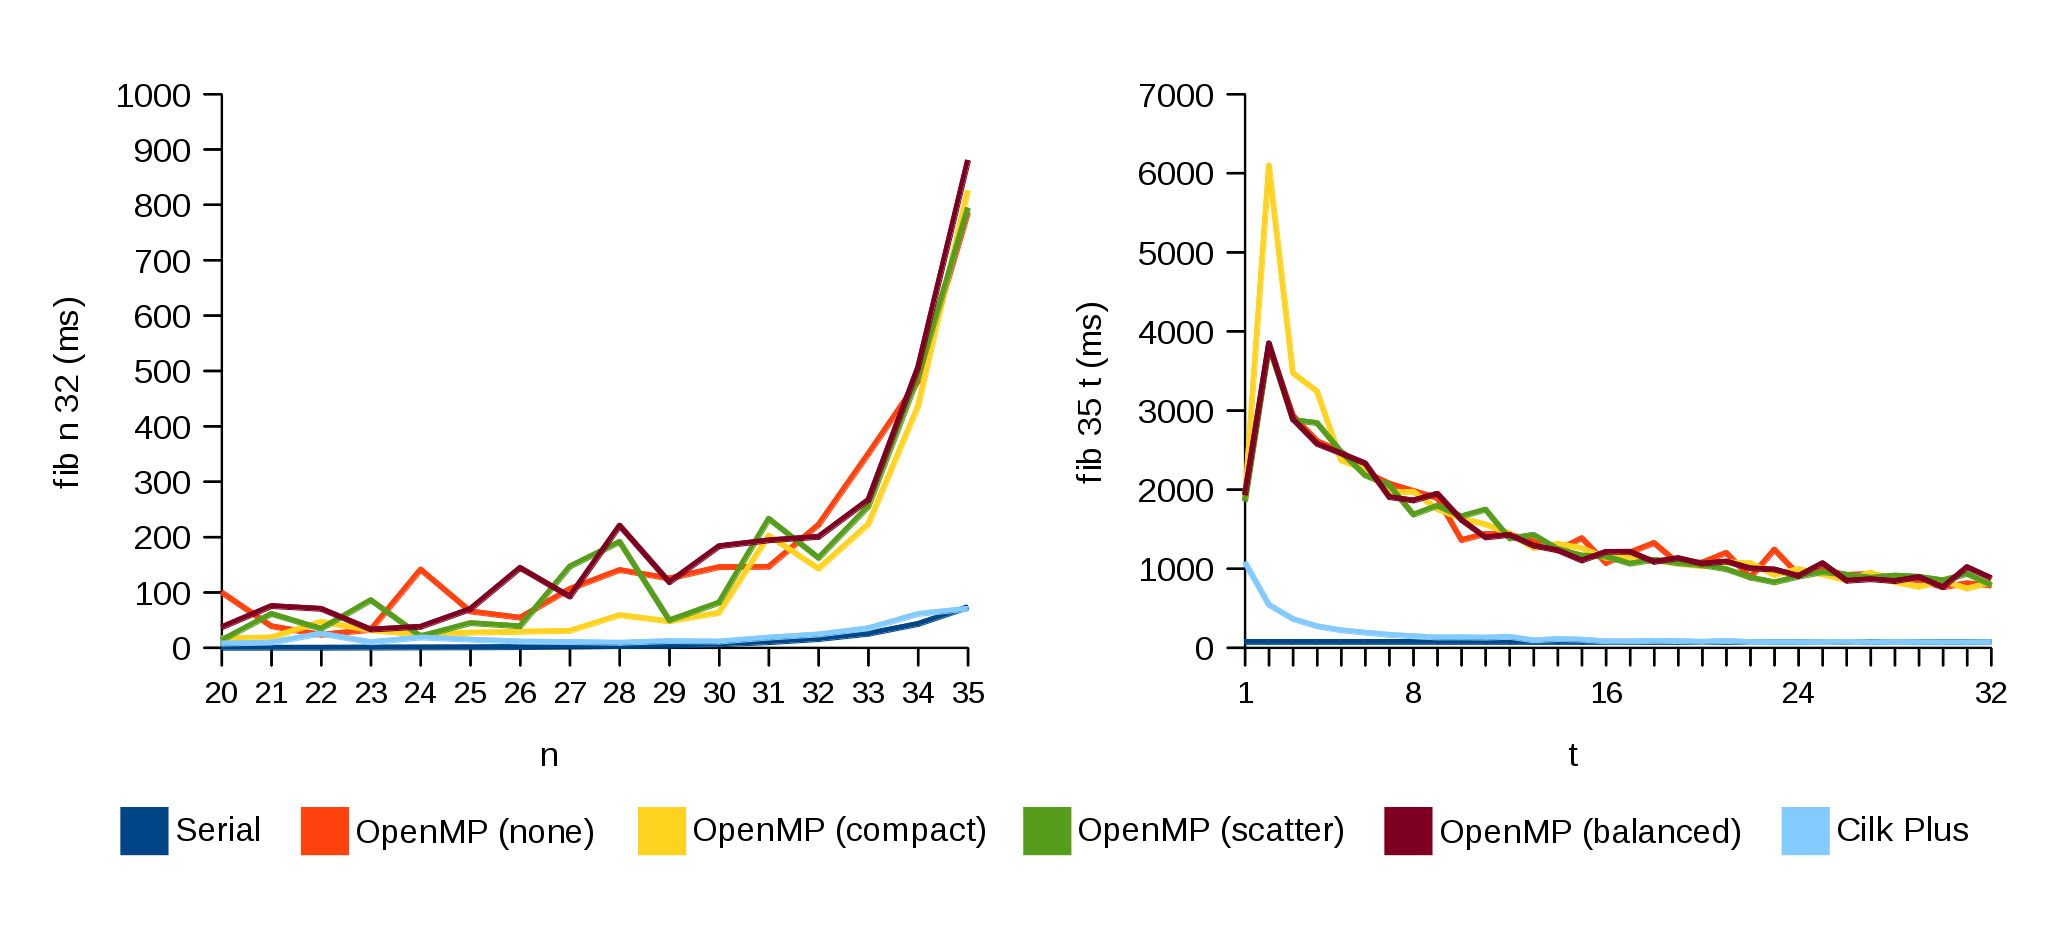
\includegraphics[width=\linewidth]{../../charts/intel64/fib_time}
	\caption{Execution time (milliseconds) of the Fibonacci benchmark on the host machine.}
	\label{Fig:fibhosttime}
\end{figure}
\noindent
\begin{figure}[h!]
	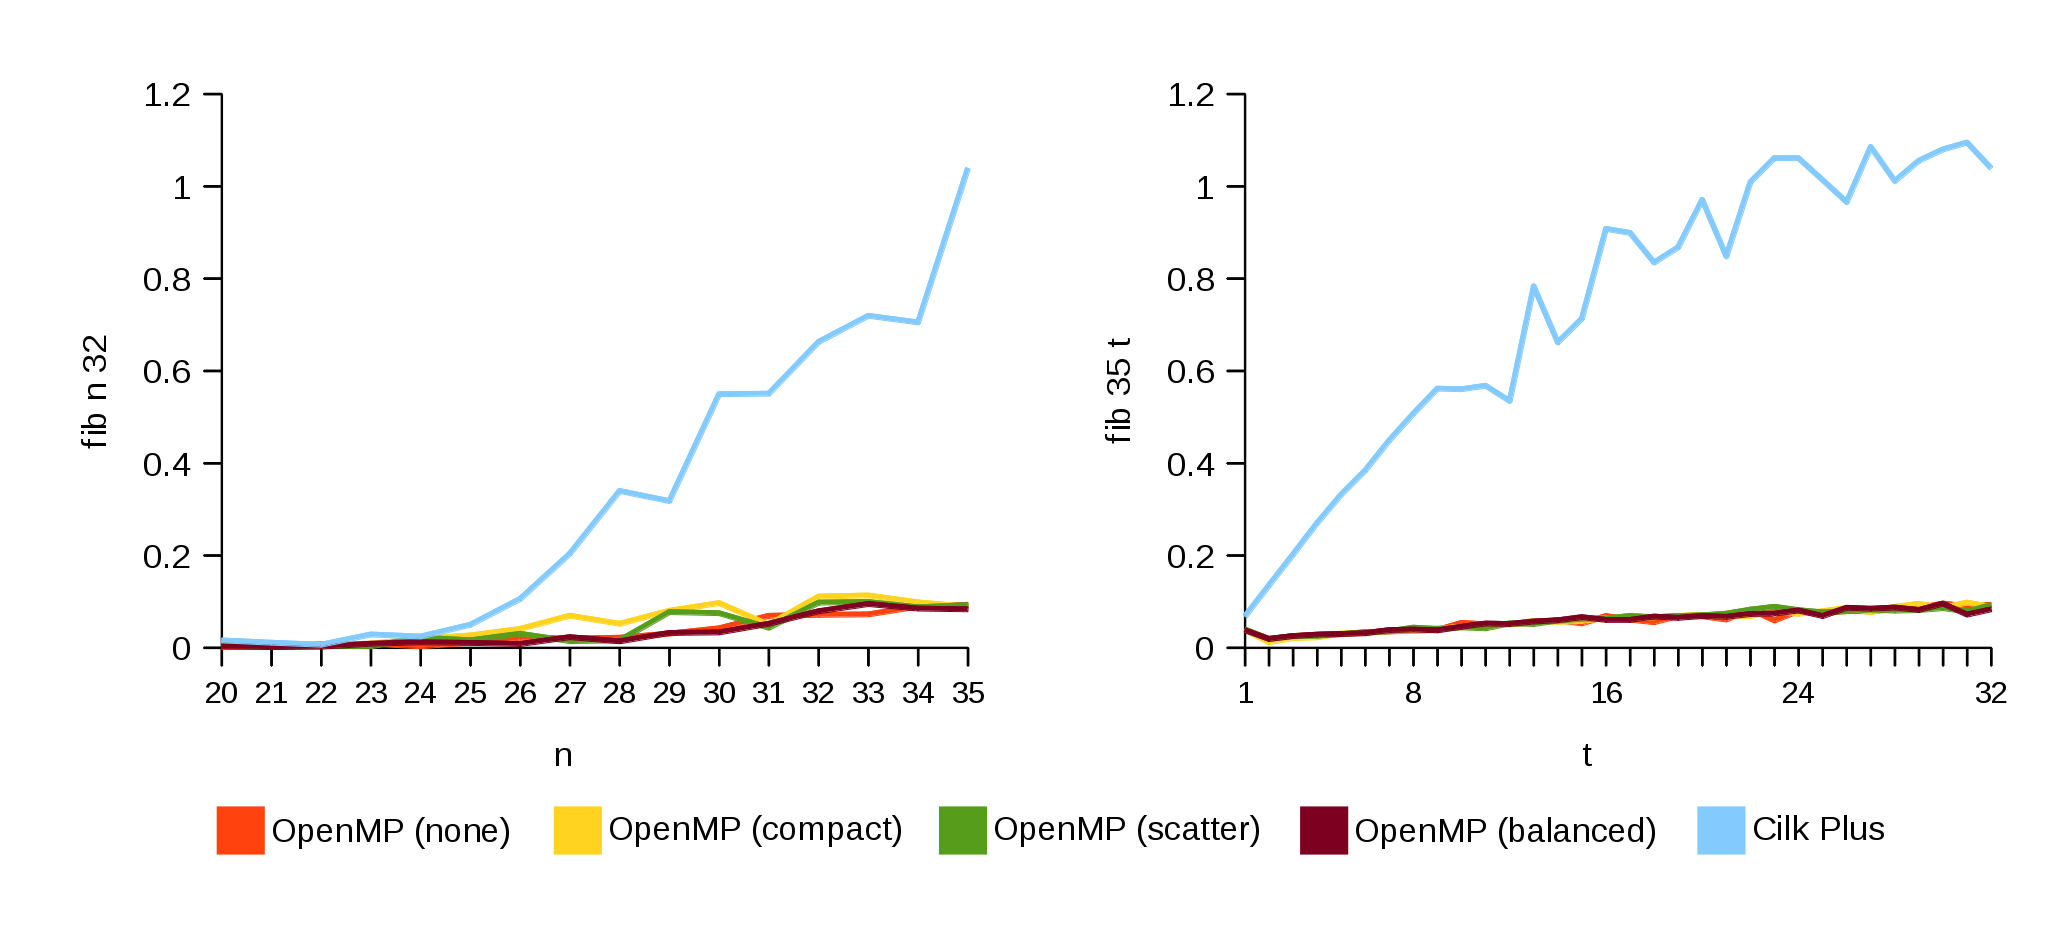
\includegraphics[width=\linewidth]{../../charts/intel64/fib_speedup}
	\caption{Speedup of the Fibonacci benchmark on the host machine.}
	\label{Fig:fibhostspeedup}
\end{figure}
Figure \ref{Fig:fibhosttime} (left) shows the relative performance of the serial, Cilk Plus and OpenMP implementations of the Fibonacci benchmark when executed on the host machine. The x-axis shows the input variable \(n\) as it is incremented through the trial range. The y-axis shows the execution time in milliseconds of each trial when the number of available threads is locked at 32 -- the maximum available on the host machine. One clear feature of the execution profile of the Fibonacci benchmark highlighted by this graph is the superior performance of the Cilk Plus implementation over OpenMP. Cilk Plus outperforms OpenMP regardless of thread affinity and for all input values. Indeed, the difference in performance increases as \(n\) is incremented, leading to a ten times performance difference between the two when \(n=35\). However, both Cilk Plus and OpenMP almost completely failed to provide any speedup over the serial implementation. Figure \ref{Fig:fibhostspeedup} (left) shows the speedup observed in the same trials over the serial implementation. Cilk Plus does appear to provide some marginal speedup over the serial trial when \(n=35\), and in future work it may be worth testing if this trend continues for higher values of \(n\).

This differs significantly from results reported in similar trials reported in the literature. Frigo \textit{et al.}\cite{Frigo98} ran a similar benchmark with \(n=35\), and found that performance improved 2.2 times with an earlier version of Cilk running on eight processors. Although not clear from their report, one cause of this difference in speedup over the serial versions running on the same computers may be latency introduced by the computers themselves. In their trial, Frigo \textit{et al.} used a Sun Enterprise 5000 SMP computer, a server with slots for multiple processors. They used eight 167 Mhz UltraSPARC processors, which have only one core and one thread per chip. In comparison, each of the two Intel Xeon processors used in the trials shown in Figure \ref{Fig:fibhosttime} contains eight cores running at 1.2 GHz, with two threads per core. One may therefore expect that the higher clock rate of the Xeon processors reduces the serial execution time to such a degree that extremely high parallelism or coarser grained tasks are needed to take advantage of the extra processors.

The OpenMP thread affinities appear to have no impact on the overall trend of the execution time as \(n\) increases, but one notable feature is that compact affinity outperforms the other strategies for almost every value of \(n\). This may be due to reduced communication latency when assigning tasks to adjacent threads as they are spawned.

Figure \ref{Fig:fibhosttime} (right) shows the relative performance of the same implementations, but this time with the input \(n\) locked to 35. The x-axis shows the number of threads used (\(t\)), from 1, equivalent to a serial implementation, to 32. Note that the serial implementation is represented by a flat line; the execution time is unchanged regardless of the number of threads used. This is a useful visualisation of how the algorithms benchmarked for this project scale to a greater number of threads. When \(t=1\), the performance difference between Cilk Plus and OpenMP is not as shown in the first graph, and all trials are slower than the serial run. Interestingly, OpenMP performance suffers a significant drop when t is increased to 2. This feature does not appear in the literature, but it may be due to a compiler optimisation that disables some or all OpenMP features if only one thread is available. The jump at \(t=2\) is most severe for compact thread affinity, but this quickly falls to similar levels as the other affinities as \(t\) is increased further. This is probably due to the scheduler attempting to utilise all threads local to a single core before moving to another. Hyper-threading is typically included in CPUs to hide the latency that occurs when performing some slow actions, such as memory or I/O operations. Compact affinity may therefore be an ineffective strategy when the number of threads used is equal to the number available on a single core, because Figure \ref{Fig:fibhosttime} suggests that using the full power of multiple cores provided better performance than splitting a single core between two workloads.

As in Figure \ref{Fig:fibhosttime} (left), Cilk Plus shows much improved performance relative to OpenMP at all values of \(t\) in Figure \ref{Fig:fibhostspeedup}. However, early gains in performance level-off after 16 threads. Figure \ref{Fig:fibhostspeedup} (right) shows this trend more clearly, with the speedup gains slowing down as more than 16 threads are applied. One key lesson that may be learned from this is that while performance gains are possible when the workload is held constant and the number of available threads raised, the actual speedup over the serial implementation on the Xeon is modest for a benchmark with granularity as fine as produced by Fibonacci. The speedup achieved by the cut-off variant, which was included to test the impact of coarser-grained tasks, is discussed in Section \ref{Sec:evalfibcutoff}.
\noindent
\begin{figure}[t!]
	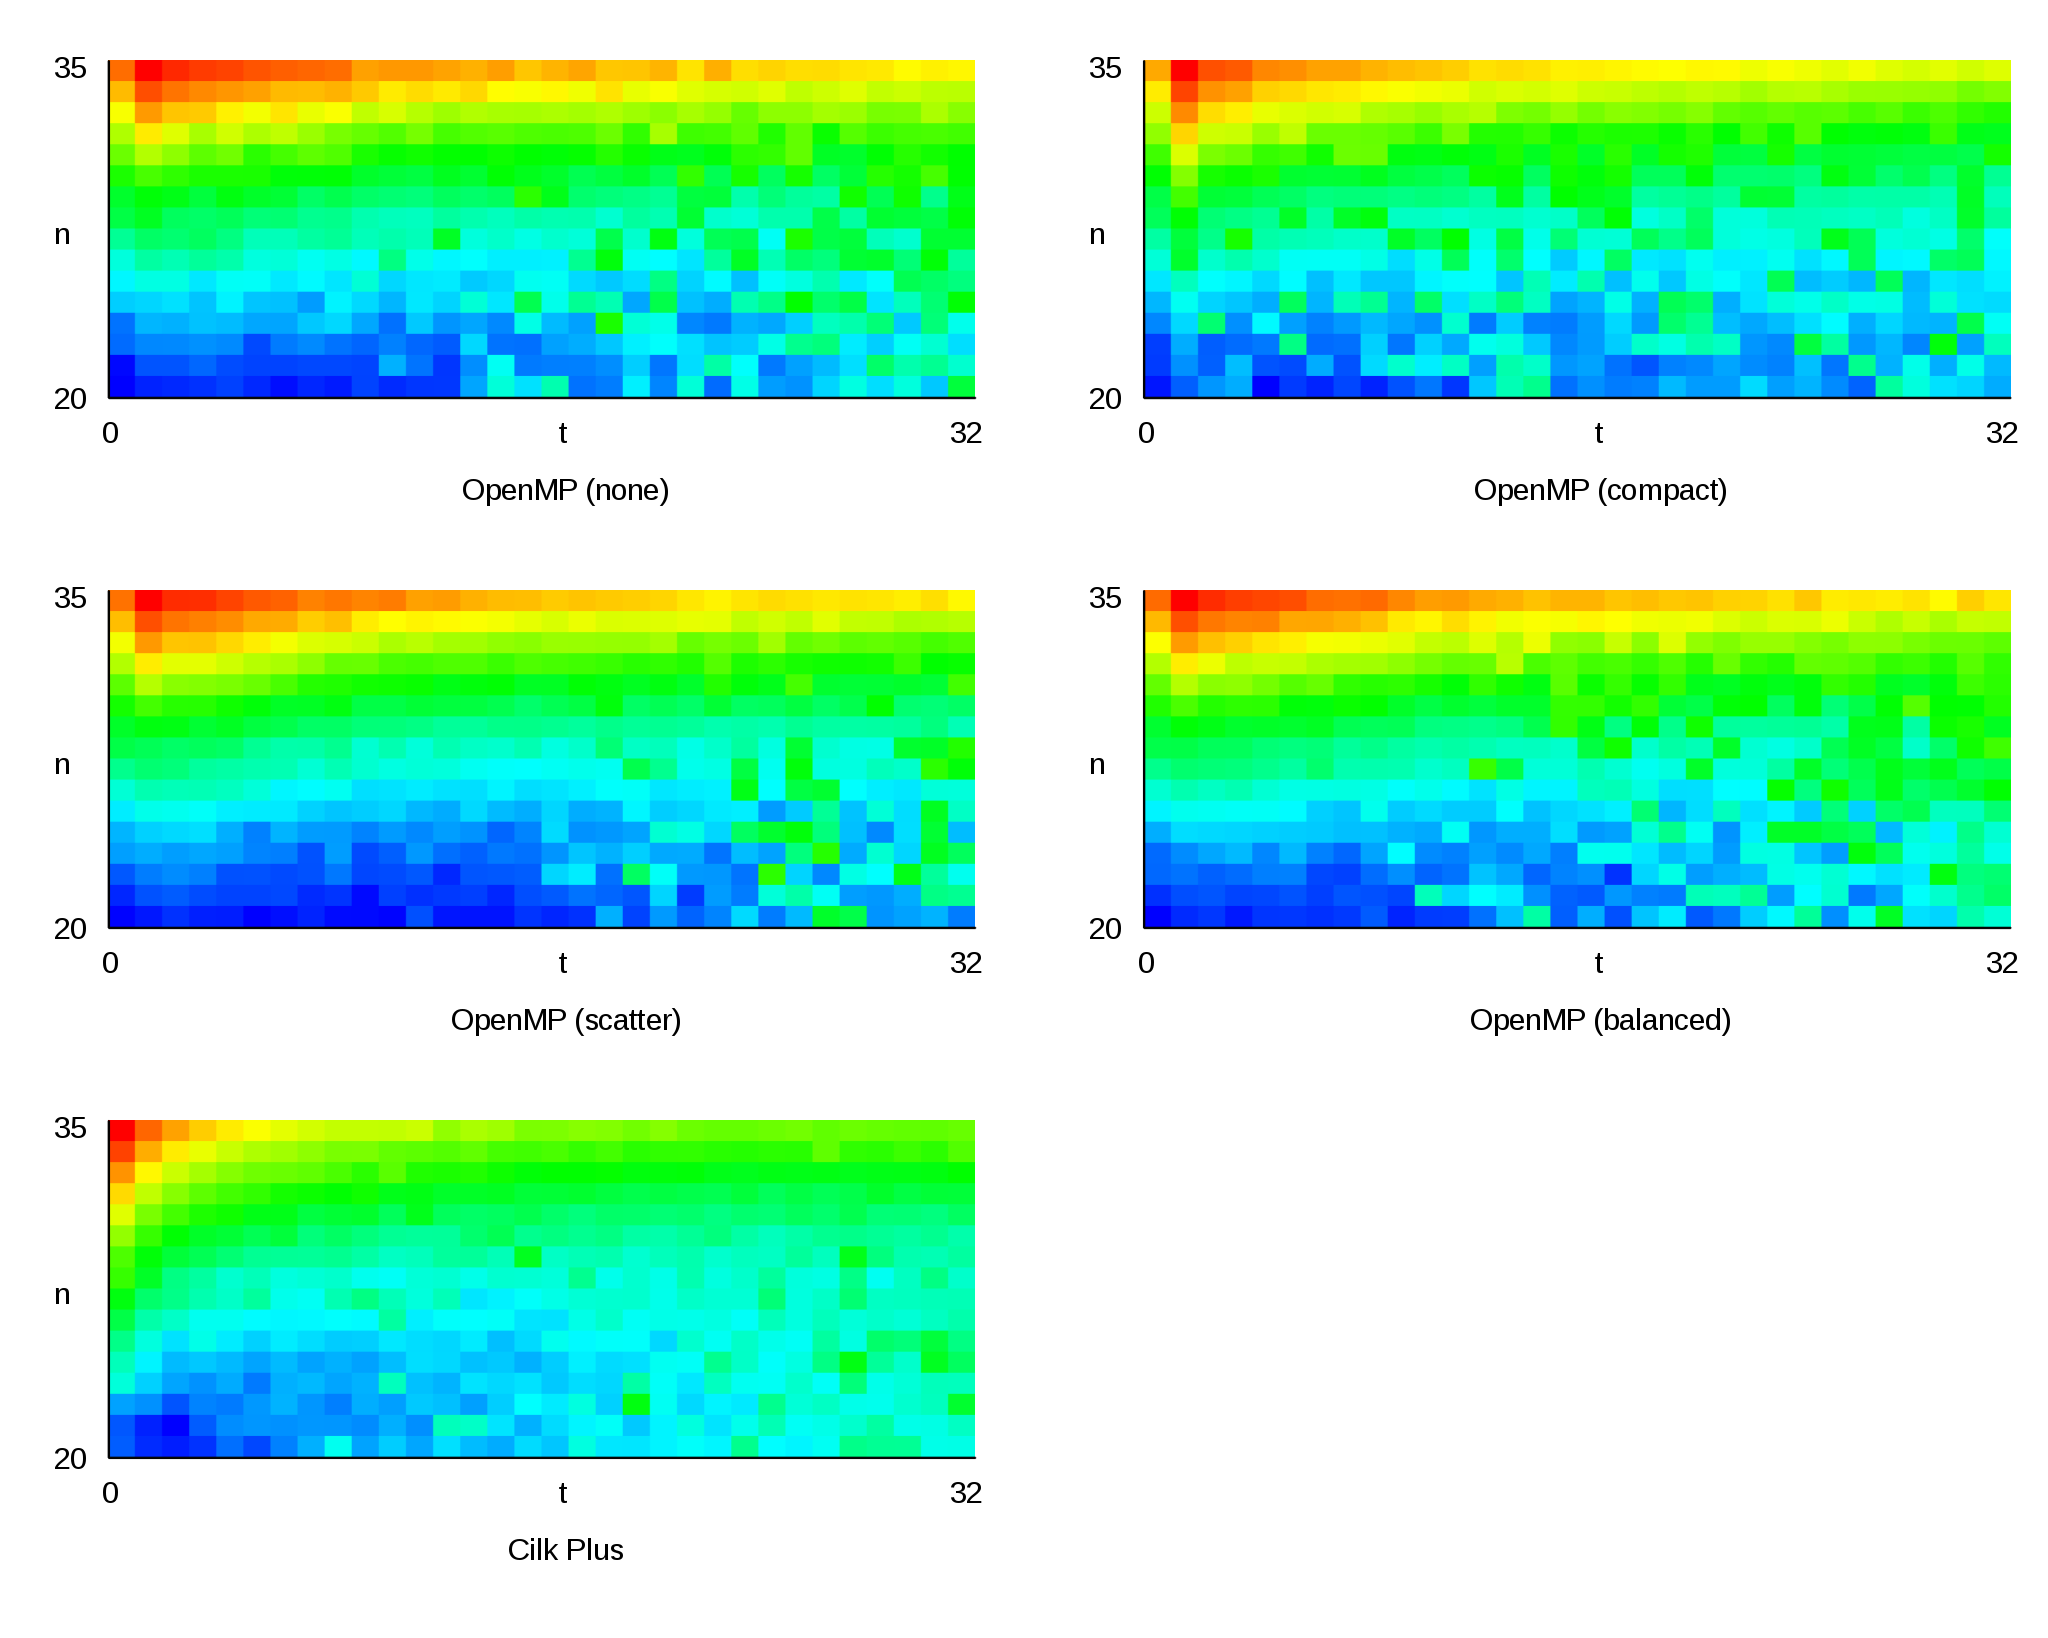
\includegraphics[width=\linewidth]{../../heatmaps/intel64/fib}
	\caption{Heatmaps showing performance spread of Fibonacci benchmark for different combinations of n and t on the host machine.}
	\label{Fig:fibhostheatmap}
\end{figure}

Figure \ref{Fig:fibhostheatmap} shows a collection of heatmaps produced for all parallel implementations of the Fibonacci benchmark when run on the host machine. The input value, \(n\), is shown on the y-axis of each heatmap, while the number of threads, \(t\), is shown on the x-axis. Blue areas indicate combinations of \(n\) and \(t\) that produced low execution times. Red areas show combinations that caused the longest execution times. As before, the similarity of the OpenMP thread affinities is visible in the overall trend of the heatmaps, with Cilk Plus a clear outlier in its performance profile. OpenMP (compact) shows more even execution times as the number of threads is increased, but all affinities show great variation for low values of \(n\). Cilk Plus shows a more consistent trend, with red areas caused by large values of \(n\) disappearing as \(t\) increases. Here it can also be seen that the small changes in execution time as \(n\) increases at \(t=35\), visible in Figure \ref{Fig:fibhosttime} (left), are also present for lower values of \(t\). However, this feature does not seem to be present for the lower values of \(t\).

\subsubsection{Xeon Phi}

Figure \ref{Fig:fibmictime} (left) shows the execution time in milliseconds of the Fibonacci benchmark on the Xeon Phi when \(t=240\) and \(n\) is incremented through the trial range. It is immediately clear that the time needed to calculate the \(n\)\textsuperscript{th} Fibonacci number on the Xeon Phi is greater than the Xeons for all implementations and at all input values. At \(n=20\), most parallel implementations exhibit execution times of between 300 and 400 milliseconds, several times greater than observed on the Xeons at \(t=30\). However, compared to the host machine, the performance difference between the serial, Cilk Plus and OpenMP implementations is relatively small, and narrows as \(n\) is increased. Indeed, Figure \ref{Fig:fibmicspeedup} (left) shows that the Cilk Plus version achieves parallel speedup greater than one at a lower value of n than was possible on the host machine. The Cilk Plus trials also exhibit a more linear trend than either the serial or OpenMP versions, which show an exponential increase in execution time as \(n\) increases. This feature may be present because of the Xeon Phi's focus on parallel computing, combined with the lower overhead of Cilk Plus.

The results for the Fibonacci benchmark on the Xeon Phi also differ from those on the host machine in that OpenMP trials using no explicit thread affinity were consistently slower than the alternatives. OpenMP compact, scatter and balanced remain within 100 ms of each other for all trials, but OpenMP (none) exceeds these by around 200 ms.
\noindent
\begin{figure}[t!]
	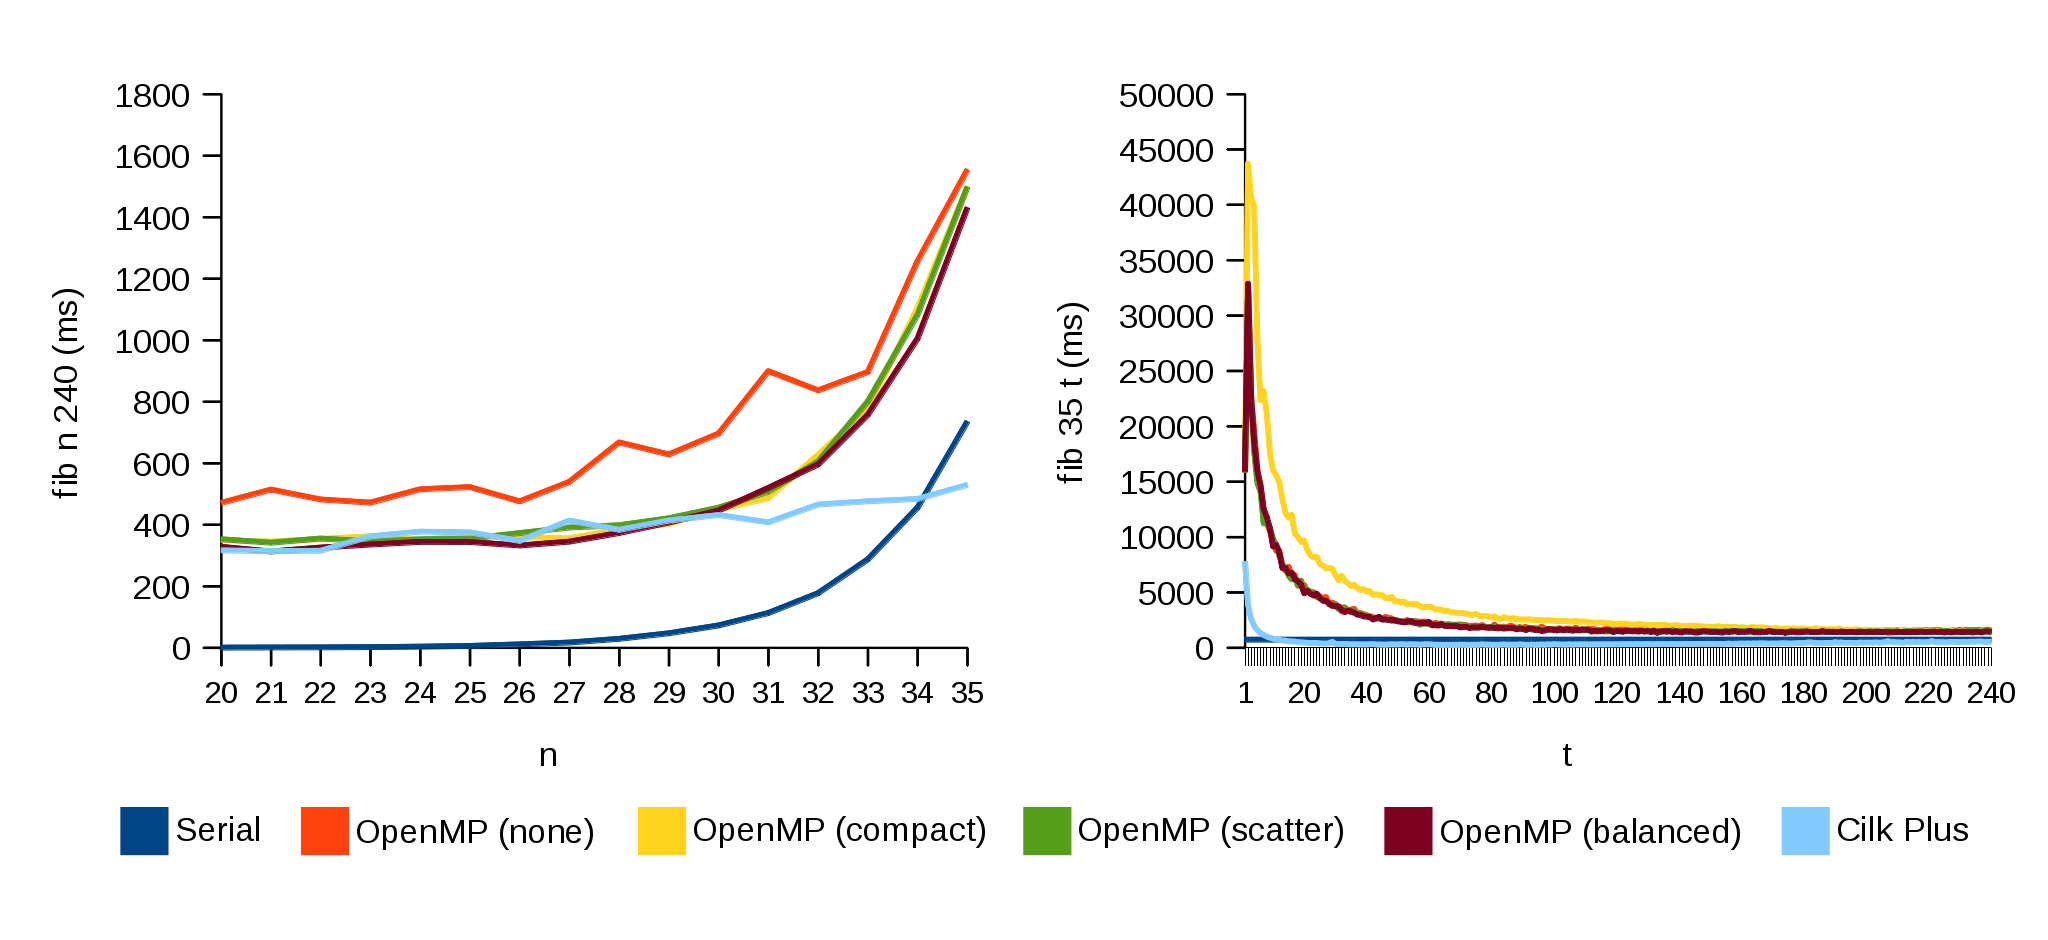
\includegraphics[width=\linewidth]{../../charts/mic/fib_time}
	\caption{Execution time (milliseconds) of the Fibonacci benchmark on the Xeon Phi.}
	\label{Fig:fibmictime}
\end{figure}
\noindent
\begin{figure}[t!]
	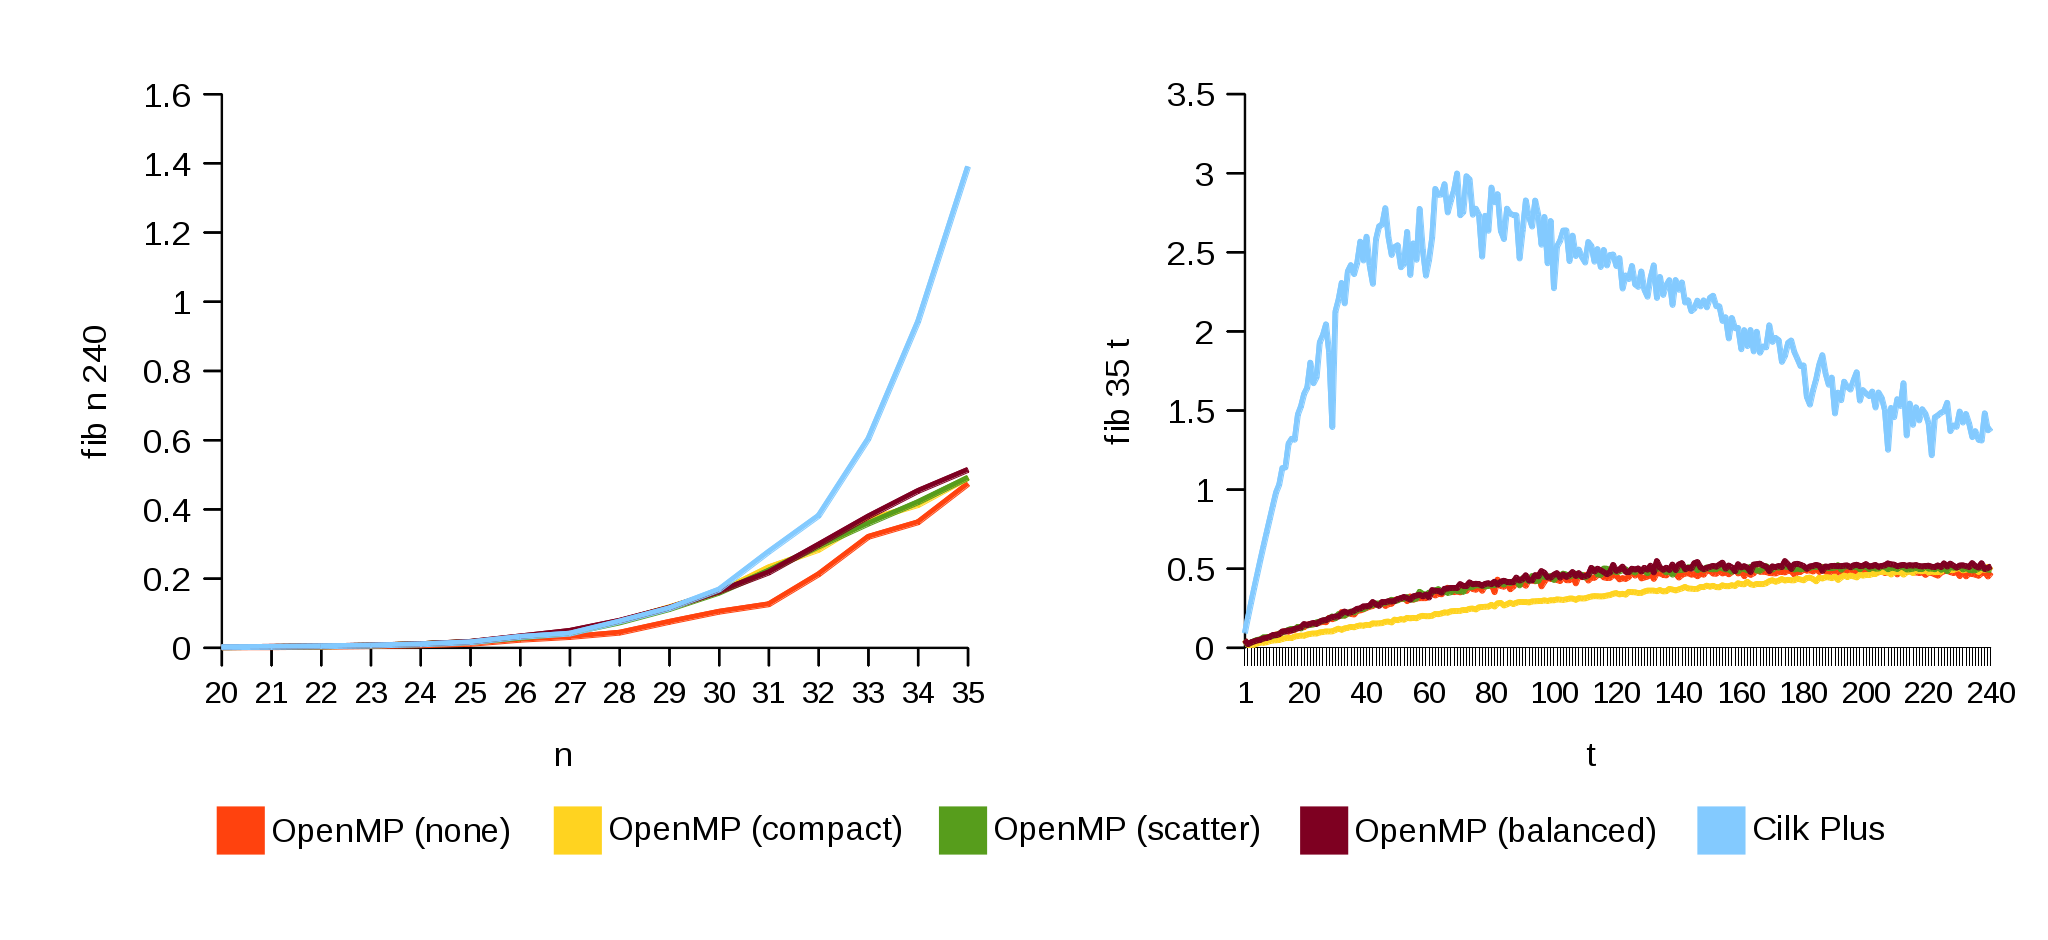
\includegraphics[width=\linewidth]{../../charts/mic/fib_speedup}
	\caption{Speedup of the Fibonacci benchmark on the Xeon Phi.}
	\label{Fig:fibmicspeedup}
\end{figure}

Figure \ref{Fig:fibmictime} (right) shows the Fibonacci benchmark executed on the Xeon Phi with \(n=35\) and \(t\) incremented from 1 to 240, the maximum number of threads available on a single Xeon Phi. The stagnation in performance after a relatively low number of threads that was seen on the host machine is also present here. Early gains up to around 100 threads do not continue at the same rate, and as one might expect from the Xeon data, this trend continues until all threads are utilised. When designing a program with fine-grained tasks like Fibonacci, therefore, the data suggests that one must be aware that increasing the number of available threads beyond a certain number does not automatically improve performance. Indeed, Figure \ref{Fig:fibmicspeedup} (right) actually shows that the Fibonacci benchmark achieved over three times speedup over the serial version on the Xeon Phi, but that this occurred when \(t\) was set to between 60 and 80. This range represents a peak in Cilk Plus' performance, beyond which speedup over the serial implementation actually fell. On the other hand, OpenMP continued to see increased speedup up to 240 threads, but always below 1.

Figure \ref{Fig:fibmicspeedup} shows the heatmaps produced by running the Fibonacci benchmark with all combinations of \(n\) and \(t\) on the Xeon Phi. Broadly, they show the same trends observed in the host machine heatmaps; Cilk Plus performs best at lower values of \(n\) and \(t\), but \(n\) has less impact on execution time as \(t\) increases. Also as before, OpenMP shows a much greater spread of colour, suggesting that it might not be able to make full use of the available threads when \(t\) is low. The variation in times observed on the host machine is also present here, but setting no OpenMP thread affinity results is much greater variation than other strategies, possibly due to a random element introduced by not explicitly specifying which threads should be used. In other words, the threads used could be executed on the same core, adjacent cores, or ``distant'' cores, so that data passed between threads is subject to more latency from the ring interconnect.
\noindent
\begin{figure}[t!]
	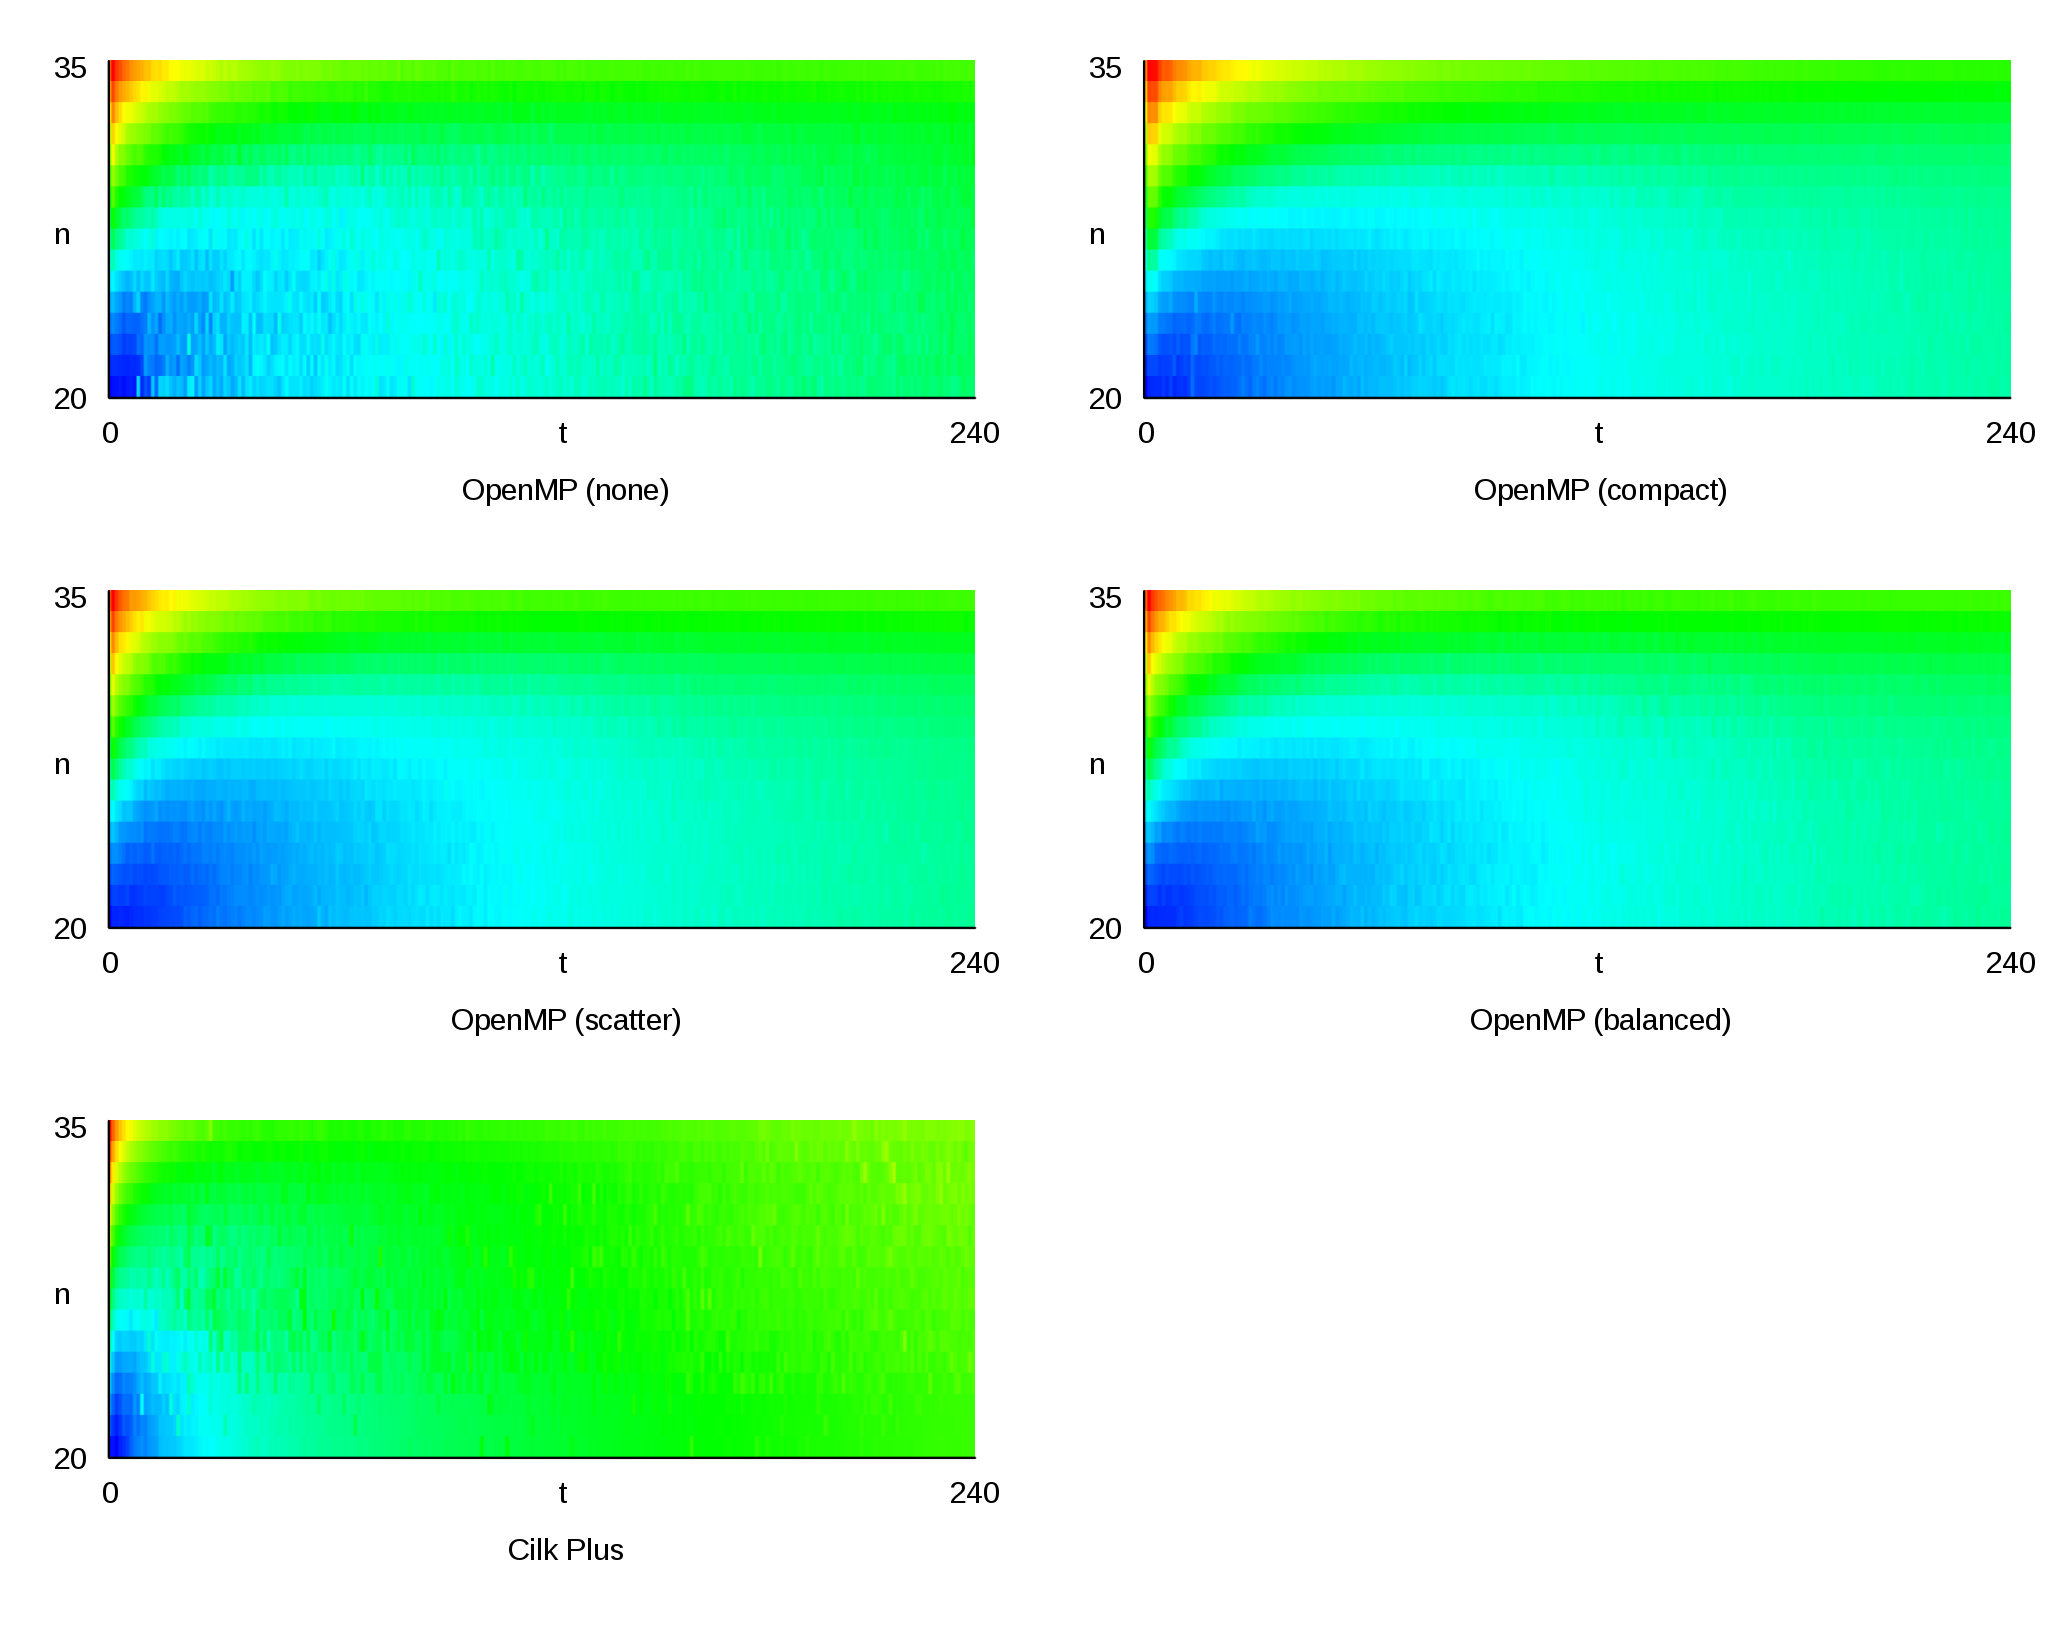
\includegraphics[width=\linewidth]{../../heatmaps/mic/fib}
	\caption{Heatmaps showing performance spread of Fibonacci benchmark for different combinations of n and t on the Xeon Phi.}
	\label{Fig:fibmicheatmap}
\end{figure}

\subsection{Cut-off} \label{Sec:evalfibcutoff}

Throughout the literature, a variant of the Fibonacci program benchmarked above, using a cut-off value, is used to increase task granularity. This section evaluates the performance of the cut-off variant on the host machine and Xeon Phi when calculating the 35\textsuperscript{th} Fibonacci number. The cut-off value \(c\) is incremented from 1 to 35, so that the tasks become more coarse-grained as c increases. A cut-off value of 1 is conceptually the same as the same trial with no cut-off; new tasks are spawned for every call to the \verb!fib! function. A cut-off value of 35 is equivalent to the serial version, since no tasks are spawned, even in the first call to \verb!fib!. Two figures are presented, one for the trials conducted on the host machine, and one for those conducted on the Xeon Phi. As before, the left chart in each figure shows the execution time in milliseconds for each trial conducted. The right chart now shows the speedup over the serial version for each trial.

\subsubsection{Host}

Figure \ref{Fig:fibcutoffhost} shows the execution time of the Fibonacci benchmark on the host machine as the cut-off value \(c\) is incremented between 1 and 35. The 35\textsuperscript{th} Fibonacci number is calculated with the maximum number of available threads. At very low values of \(c\), Figure \ref{Fig:fibcutoffhost} (left) shows performance for all libraries and thread affinities similar to that observed for \(n=35\) with no cut-off. This quickly improves as \(c\) increases and the lower levels of the task graph become serialised. All frameworks and affinities achieved speedup over the serial version for some \(c\) between 10 and 30. As before, Cilk Plus demonstrates better performance than OpenMP in the Fibonacci benchmark, but it also shows more consistency. When the Cilk Plus version reaches a performance plateau at around \(c=5\), only slight variations can be seen. In comparison, the OpenMP trials achieve a performance plateau in a broad sense, but shows huge variations within the same range. This is despite three separate trials for each combination of inputs, indicating the particular sets of inputs are producing anomalous performance, perhaps due to a feature of the hardware. As \(c\) approaches 35, the Cilk Plus and OpenMP versions see their speedup cut, and the additional overhead induced by parallelisation causes their execution time at \(c=35\) to lie above the serial implementation. At this point, the parallel versions do not spawn new tasks, and are executing code similar to their serial elision.
\noindent
\begin{figure}[t!]
	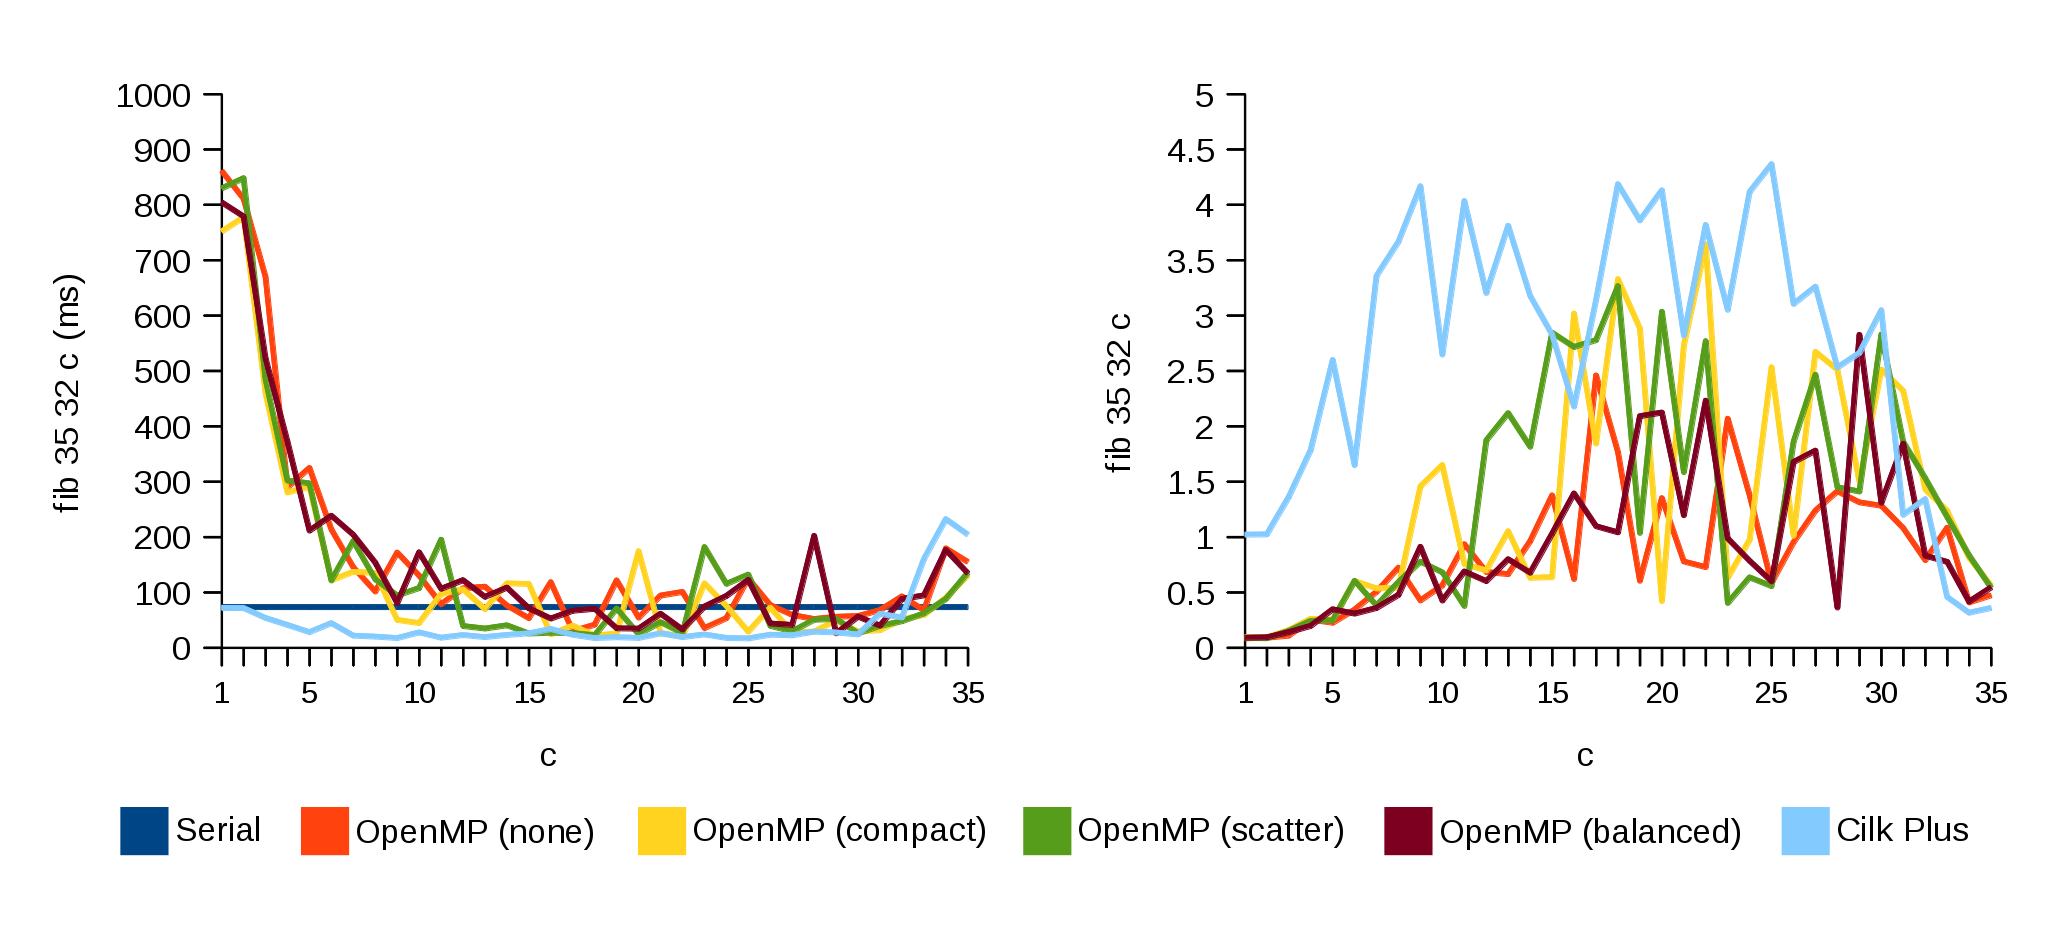
\includegraphics[width=\linewidth]{../../charts/intel64/fib_cutoff}
	\caption{Execution time (left) and speedup (right) of the Fibonacci benchmark with cut-off on the host machine.}
	\label{Fig:fibcutoffhost}
\end{figure}

\subsubsection{Xeon Phi}

Figure \ref{Fig:fibcutoffmic} (right) shows the cut-off variant when run on the Xeon Phi using all 240 threads. Similar to the standard version, the Xeon Phi takes longer to compute the 35\textsuperscript{th} Fibonacci number for all frameworks and thread affinities than the host machine. However, the speedup achieved (right) is more consistent for both Cilk Plus and OpenMP, and even the worst performing thread affinity, none, maintains a speedup greater than 1 until \(c=33\). The same trials on the host machine often dipped below 1. Cilk Plus shows almost no change in performance as \(c\) increases, until it and OpenMP converge on almost the same point when \(c\) approaches 35. This may be caused by additional work imposed by the if-statement needed to check the cut-off value.
\noindent
\begin{figure}[t!]
	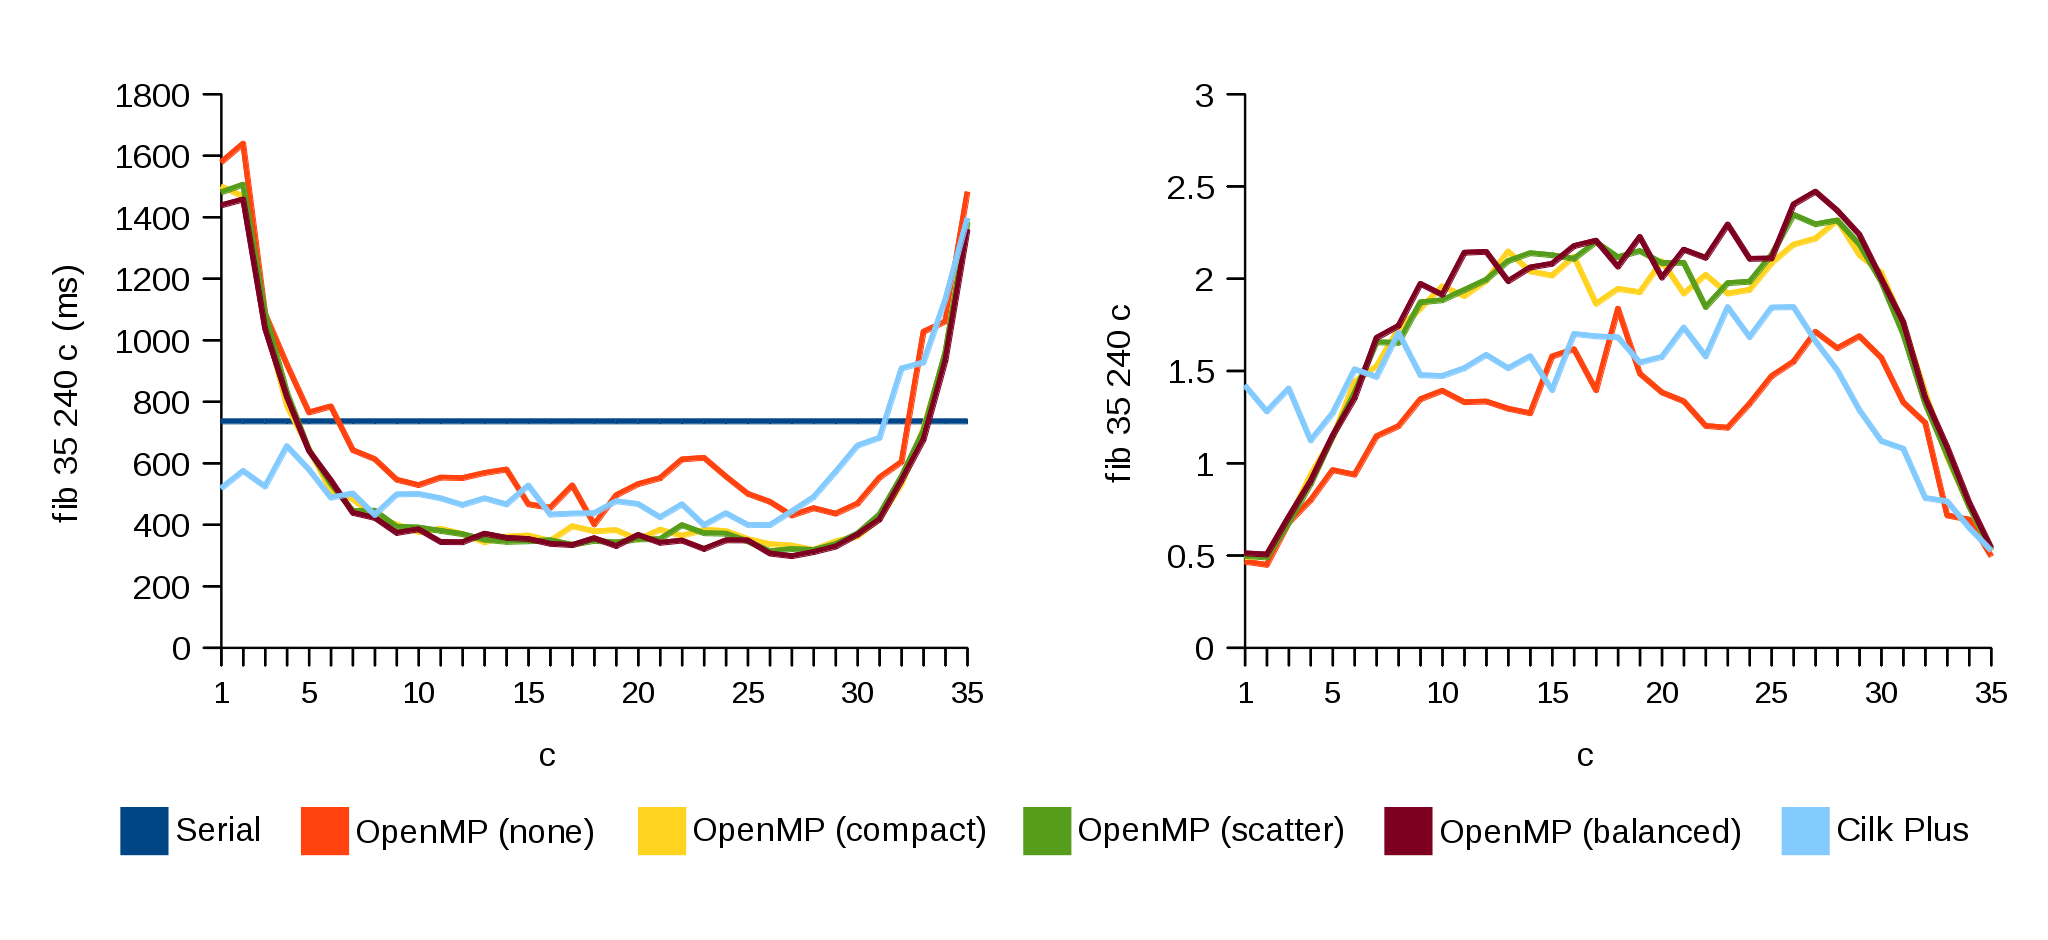
\includegraphics[width=\linewidth]{../../charts/mic/fib_cutoff}
	\caption{Execution time (left) and speedup (right) of the Fibonacci benchmark with cut-off on the Xeon Phi.}
	\label{Fig:fibcutoffmic}
\end{figure}

\subsubsection{Comparison}

Compared with the standard version of the Fibonacci benchmark evaluated in Section \ref{Sec:evalfibstandard}, the cut-off variant shows much greater performance when \(c\) lies between 10 and 30. This is true for trials on both the host machine and Xeon Phi. However, compared with the results produced by Olivier \textit{et al.}\cite{Olivier12}, the performance presented for the Fibonacci benchmark in this report is relatively poor. They saw speedup of around 20 times on a 32-core machine, while the 32-threads of the host machine only achieved four times, and the Xeon Phi even less. Tousimojarad and Vanderbauwhede\cite{Tousimojarad14} used the cut-off variant to achieve almost 100 times speedup on the Xeon Phi in the best case, totally different results than shown in Figure \ref{Fig:fibcutoffmic}, in which the Xeon Phi provides very little benefit over running the benchmark on a single thread. This may be due to differences not specified in their paper. However, they did observe some similar features; notably, that the performance of OpenMP falls when more threads are made available. They also present load-balancing data gathered with the Intel VTune Amplifier XE tool, noting that Cilk Plus does a better job of balancing the work-load it is presented, ultimately achieving higher performance than any OpenMP thread affinity when the cut-off value is large. The results presented by Podobas \textit{et al.}\cite{Podobas15} are somewhat more in line with those presented here. On a 64-core many-core processor, they show performance gains closer to 30 times when 40-50 threads are used. This is still significantly different from the speedup observed in this report on either the host machine or Xeon Phi.

\section{Merge Sort} \label{Sec:evalmsort}

This section presents the results of the merge sort benchmark. As with Fibonacci, the results of the standard version of presented first, followed by the powers-of-two trials. Particular attention is paid to notable patterns that emerged, and an attempt made to explain their presence.

\subsection{Standard Version} \label{Sec:evalmsortstandard}

\subsubsection{Host}

Figure \ref{Fig:msorthosttime} (left) shows the serial, OpenMP and Cilk Plus versions of the merge sort benchmark executed on the host machine. The maximum number of threads is used, and the size of the array to be sorted increased from 0.1 million to 3 million in increments of 0.1 million. Figure \ref{Fig:msorthostspeedup} (left) shows the same trials in terms of speedup over the serial implementation. One reassuring feature that appears in the first chart is the apparently linear trend of the serial implementation as \(n\) increases. This is expected from the known \(O(nlogn)\) performance of the merge sort, and indicates that the implementation is working as intended. Cilk Plus achieves speedup over the serial version almost immediately, and settles into a similarly linear trend, but at a much shallower angle, indicating strong parallelism. This results in the Cilk Plus implementation achieving gradually better performance than the serial version throughout the trial range. Figure \ref{Fig:msorthostspeedup} (left) shows Cilk achieving speedup of around five times when the array contains three million integers. This is contrasted with OpenMP, which does not immediately provide any benefit over the serial implementation, but maintains a shallower angle and eventually provides around two times speedup when \(n=3m\). Although following the same broad trend, all OpenMP thread affinities show large variations in performance throughout the trial range. The scatter affinity, for example, is at different times both the best and worst performing affinity.

Figure \ref{Fig:msorthosttime} (right) shows the serial, OpenMP and Cilk Plus versions of the merge benchmark when different numbers of threads are used to sort an array with three million integers. The same performance plateau that appeared in the Fibonacci benchmark is present here, but additional threads beyond \(t=16\) do seem to cause continued improvement, especially for OpenMP. Another similarity is that the compact thread affinity spikes when two threads are used, due to underutilisation of the available physical cores. Further differences between the OpenMP thread affinities may be hidden in noise, despite the data being generated from three runs for each combination of inputs and the average taken. Both Cilk Plus and OpenMP achieve their best performance when the maximum number of threads are used, indicating that the merge sort algorithm scales well in a highly parallel environment.
\noindent
\begin{figure}[t!]
	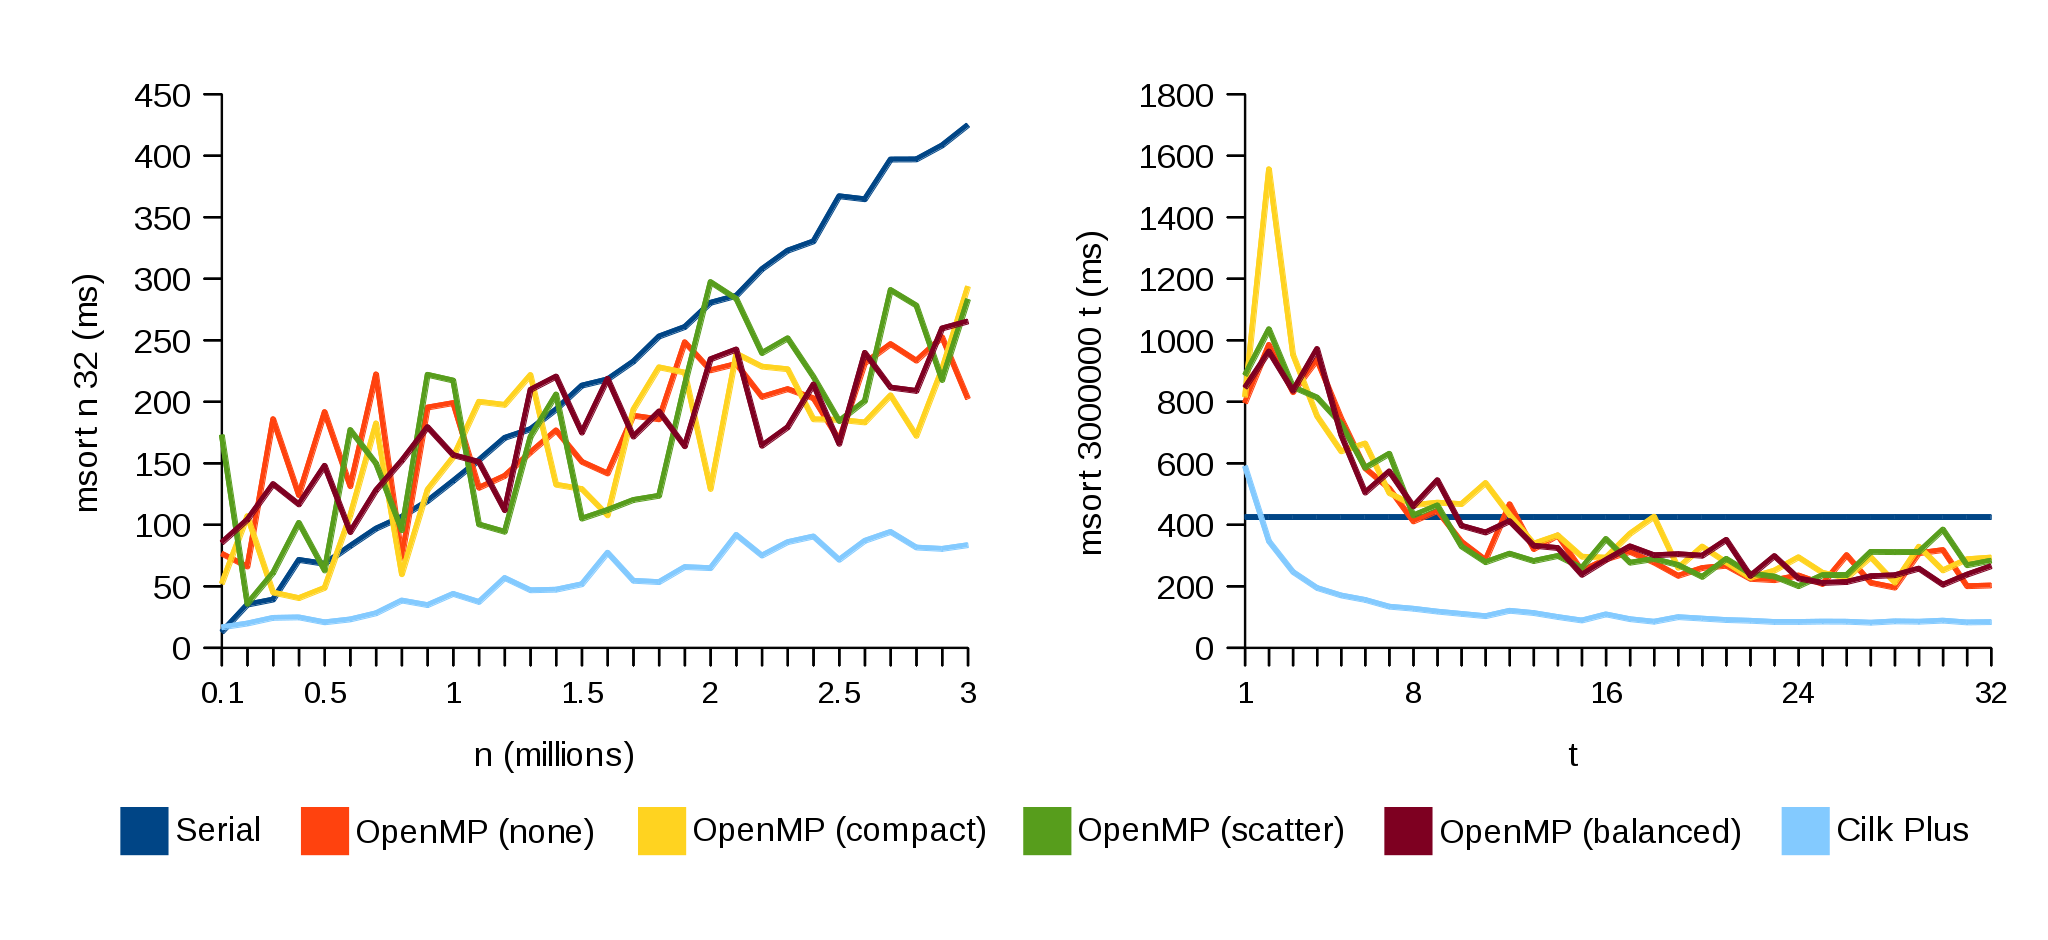
\includegraphics[width=\linewidth]{../../charts/intel64/msort_time}
	\caption{Execution time (milliseconds) of the merge sort benchmark on the host machine.}
	\label{Fig:msorthosttime}
\end{figure}
\noindent
\begin{figure}[t!]
	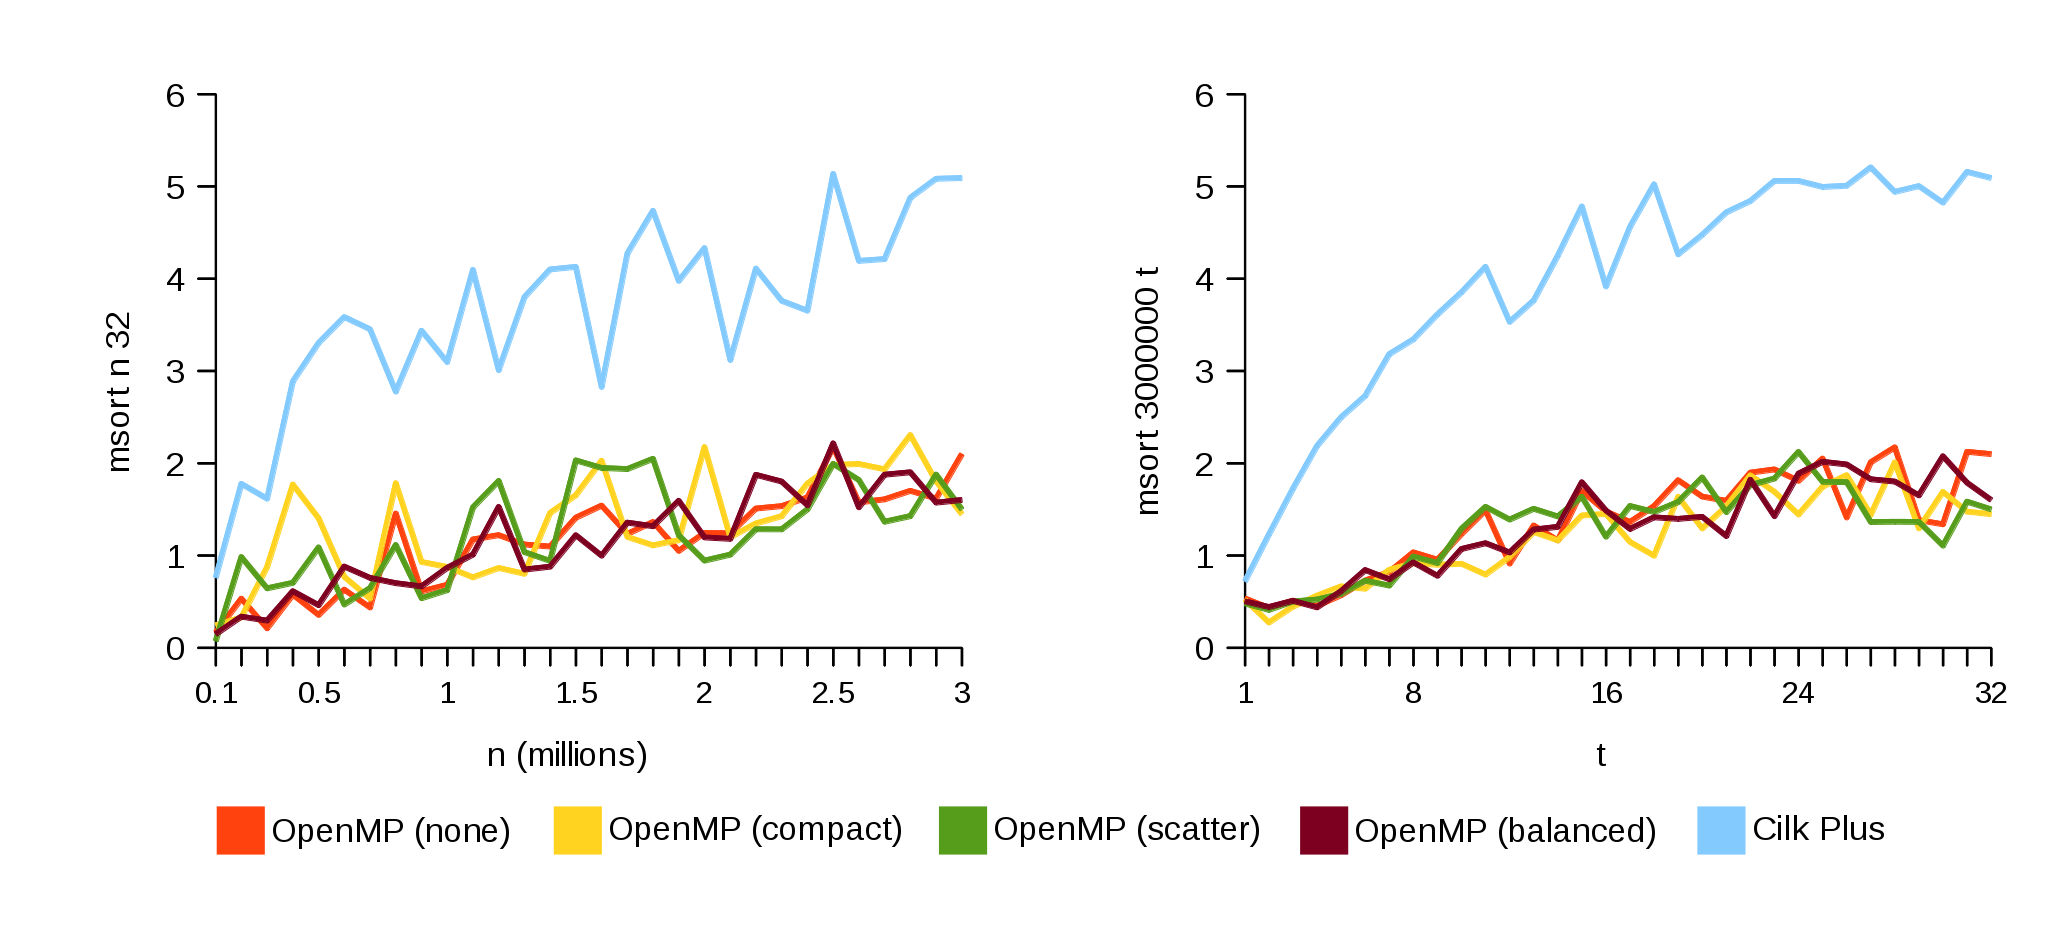
\includegraphics[width=\linewidth]{../../charts/intel64/msort_speedup}
	\caption{Speedup of the merge sort benchmark on the host machine.}
	\label{Fig:msorthostspeedup}
\end{figure}

Figure \ref{Fig:msorthostheatmap} shows a collection of heatmaps produced by recording the execution time of the merge sort benchmark at every combination of \(n\) and \(t\). The difference between the different OpenMP thread affinities is shown clearer here; compact appears to show worse performance than the others when \(t\) is low, before providing more even performance when more threads are made available, but this may be due to the single spike observed in Figure \ref{Fig:msorthosttime} (right) causing the colouring of the heatmap to be inconsistent with the other OpenMP trials. This highlights a flaw in the technique used to generate the heatmaps, where the colour scale is interpolated linearly between the highest and lowest values in a single set of trials, rather than producing heatmaps consistent across all trials. The Cilk Plus trials are again characterised by much more consistent performance across all values of \(n\) and \(t\), while OpenMP only appears to be consistent within a small linear range of inputs when \(t<16\) and \(n<1.5\)M. Despite these differences, a feature that appears in every heatmap is an area of blue at low values of \(n\) and all values of \(t\). This indicates that the time taken to sort a small array changes little, regardless of the number of threads utilised. This may be a performance bottleneck caused by parallel overhead, suggesting that much larger arrays should be used to make the most of parallel hardware, which is consistent with the finding in the previous figures.
\noindent
\begin{figure}[t!]
	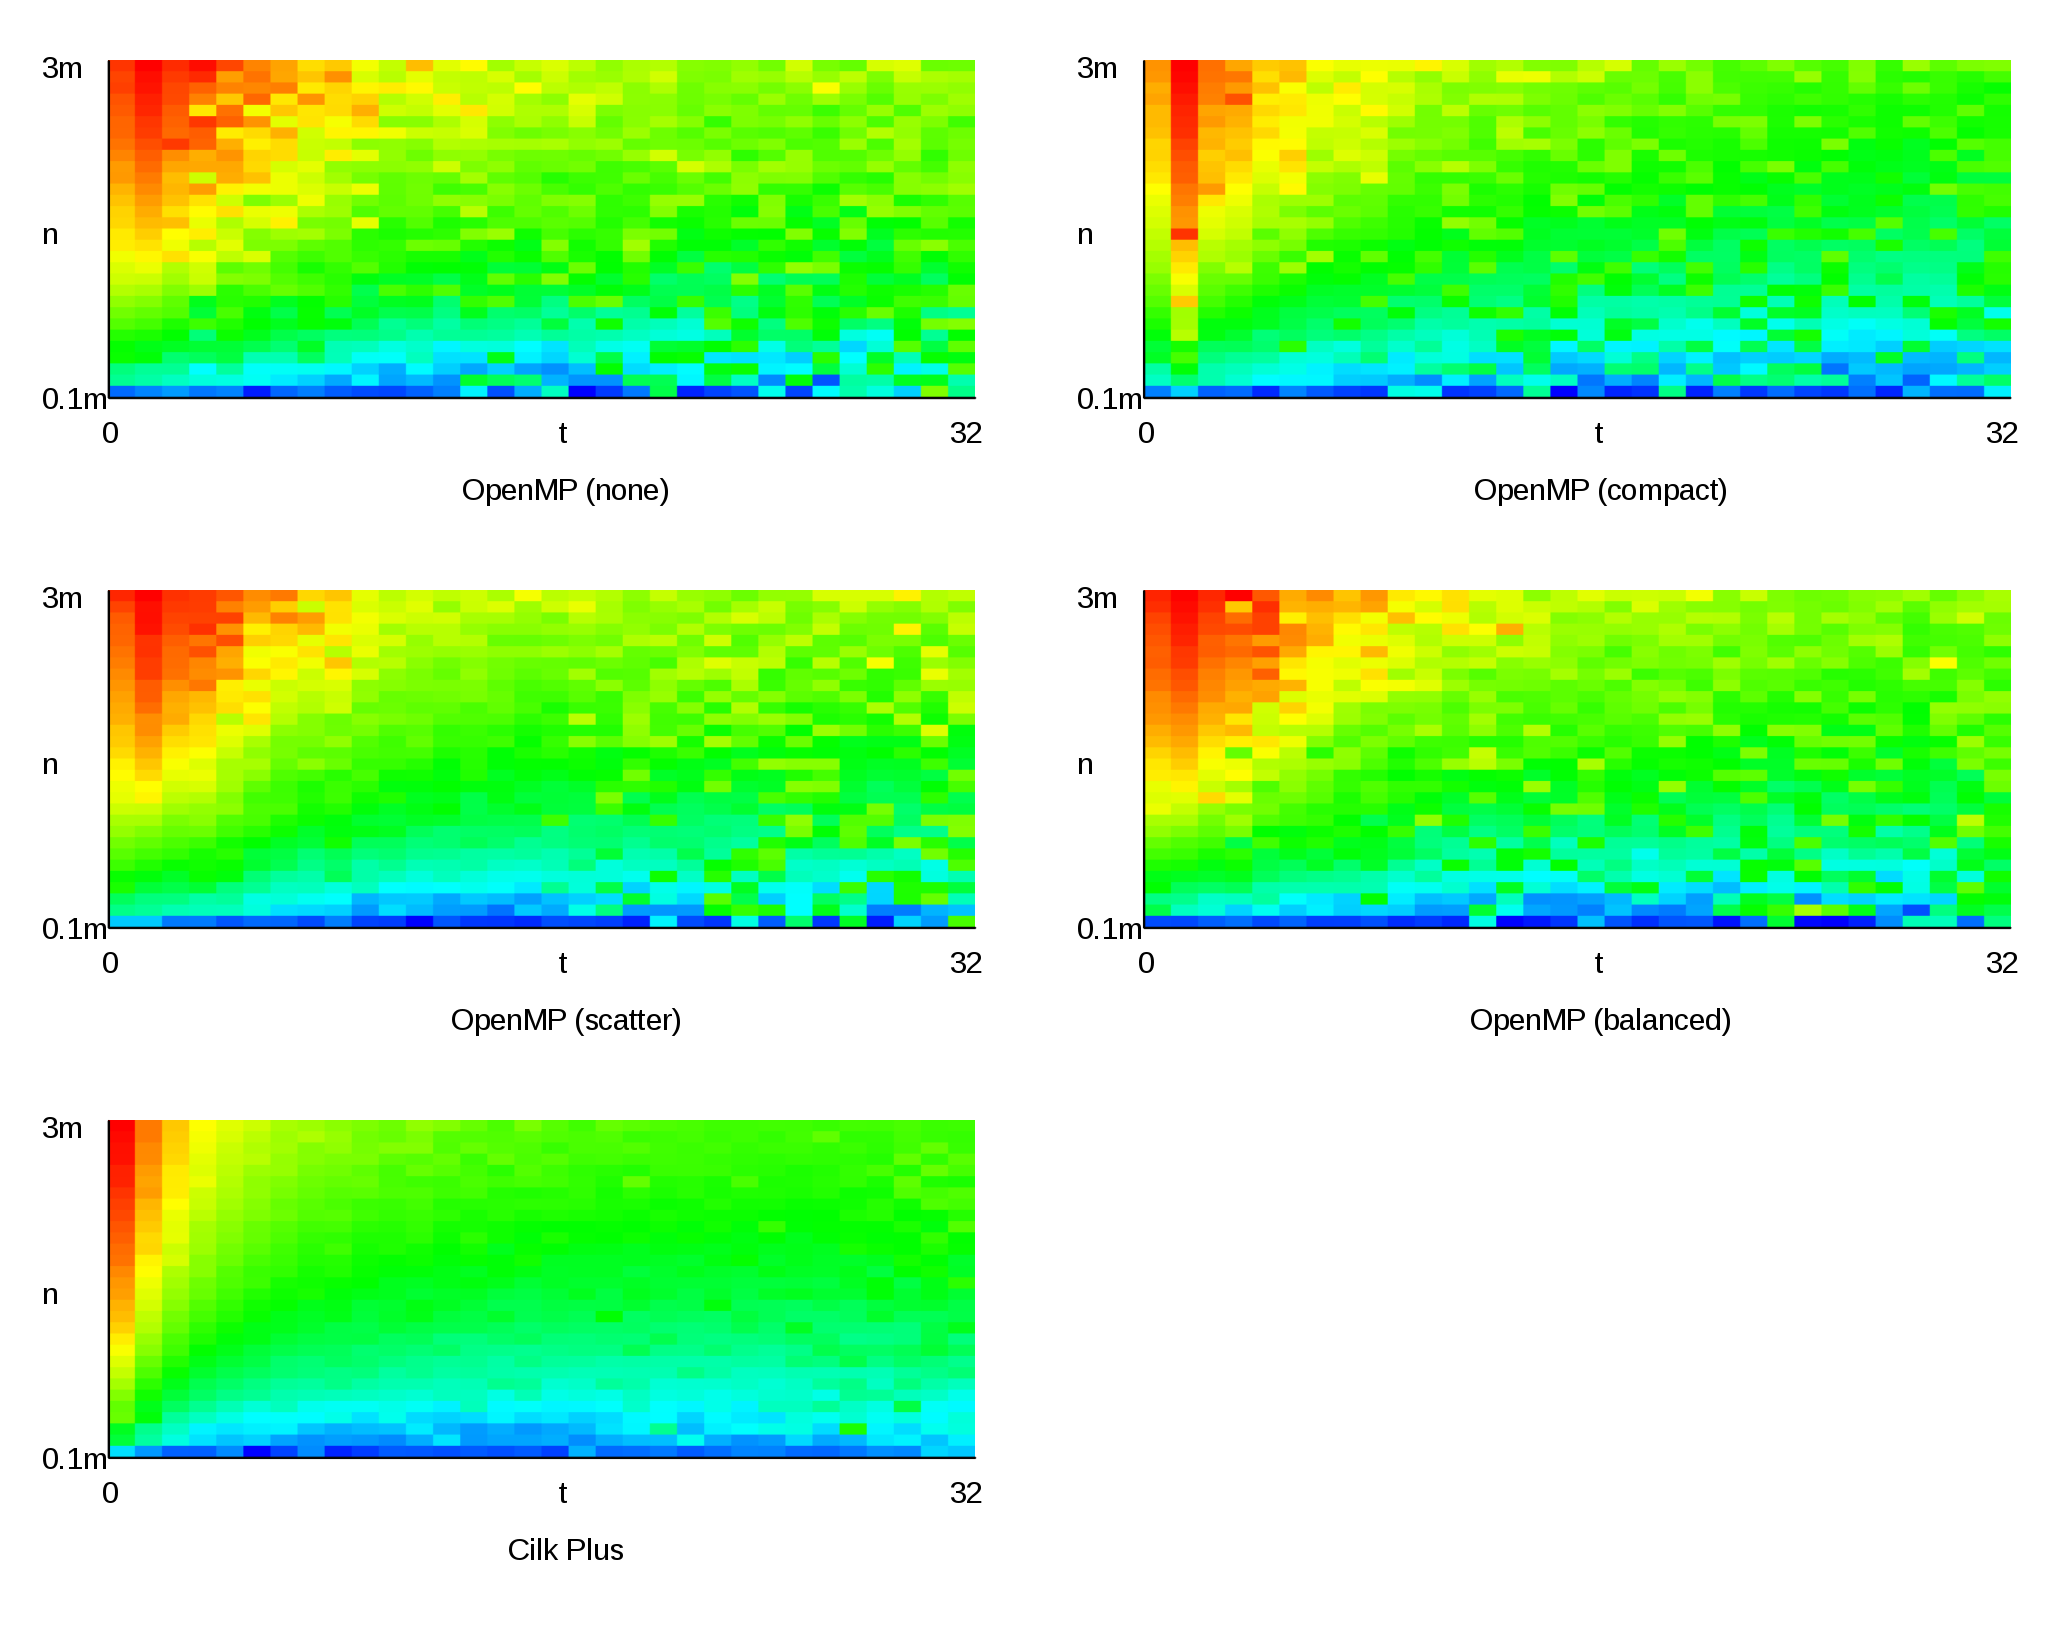
\includegraphics[width=\linewidth]{../../heatmaps/intel64/msort}
	\caption{Heatmaps showing performance spread of merge sort benchmark for different combinations of n and t on the host machine.}
	\label{Fig:msorthostheatmap}
\end{figure}

\subsubsection{Xeon Phi}

Figure \ref{Fig:msortmictime} shows the performance of the serial, OpenMP and Cilk Plus versions of the merge sort benchmark executed on the Xeon Phi. Figure \ref{Fig:msortmicspeedup} shows the speedup achieved by each parallel implementation relative to the serial implementation. The same \(O(nlogn)\) trend that was present for the serial implementation on the host machine is also present in Figure \ref{Fig:msortmictime} (left), as is the similarly linear trend of the parallel versions. However, in comparison with the performance of the host machine, Cilk Plus shows significantly worse performance than all OpenMP variants. For small input arrays, all implementations perform around fifty times slower than when run on the host machine, although this difference is less severe for  the largest arrays, falling to around two times slower. This is an interesting trend, because it indicates that although the Xeon Phi appears to provide worse performance for small data sets, much larger arrays may be sorted faster on the Xeon Phi. Indeed, many results presented in the literature were produced by sorting arrays of 80 million integers or more\cite{Tousimojarad14}. Differences between OpenMP thread affinities are much clearer on the Xeon Phi, with more consistent results making the data easier to read. Setting no thread affinity causes a performance decrease of around 200 ms, while explicitly setting any of the other affinity options appears to have little impact. Unlike the Fibonacci benchmark, OpenMP achieved the best performance when 240 threads were used, at around a three times speedup.
\noindent
\begin{figure}[t!]
	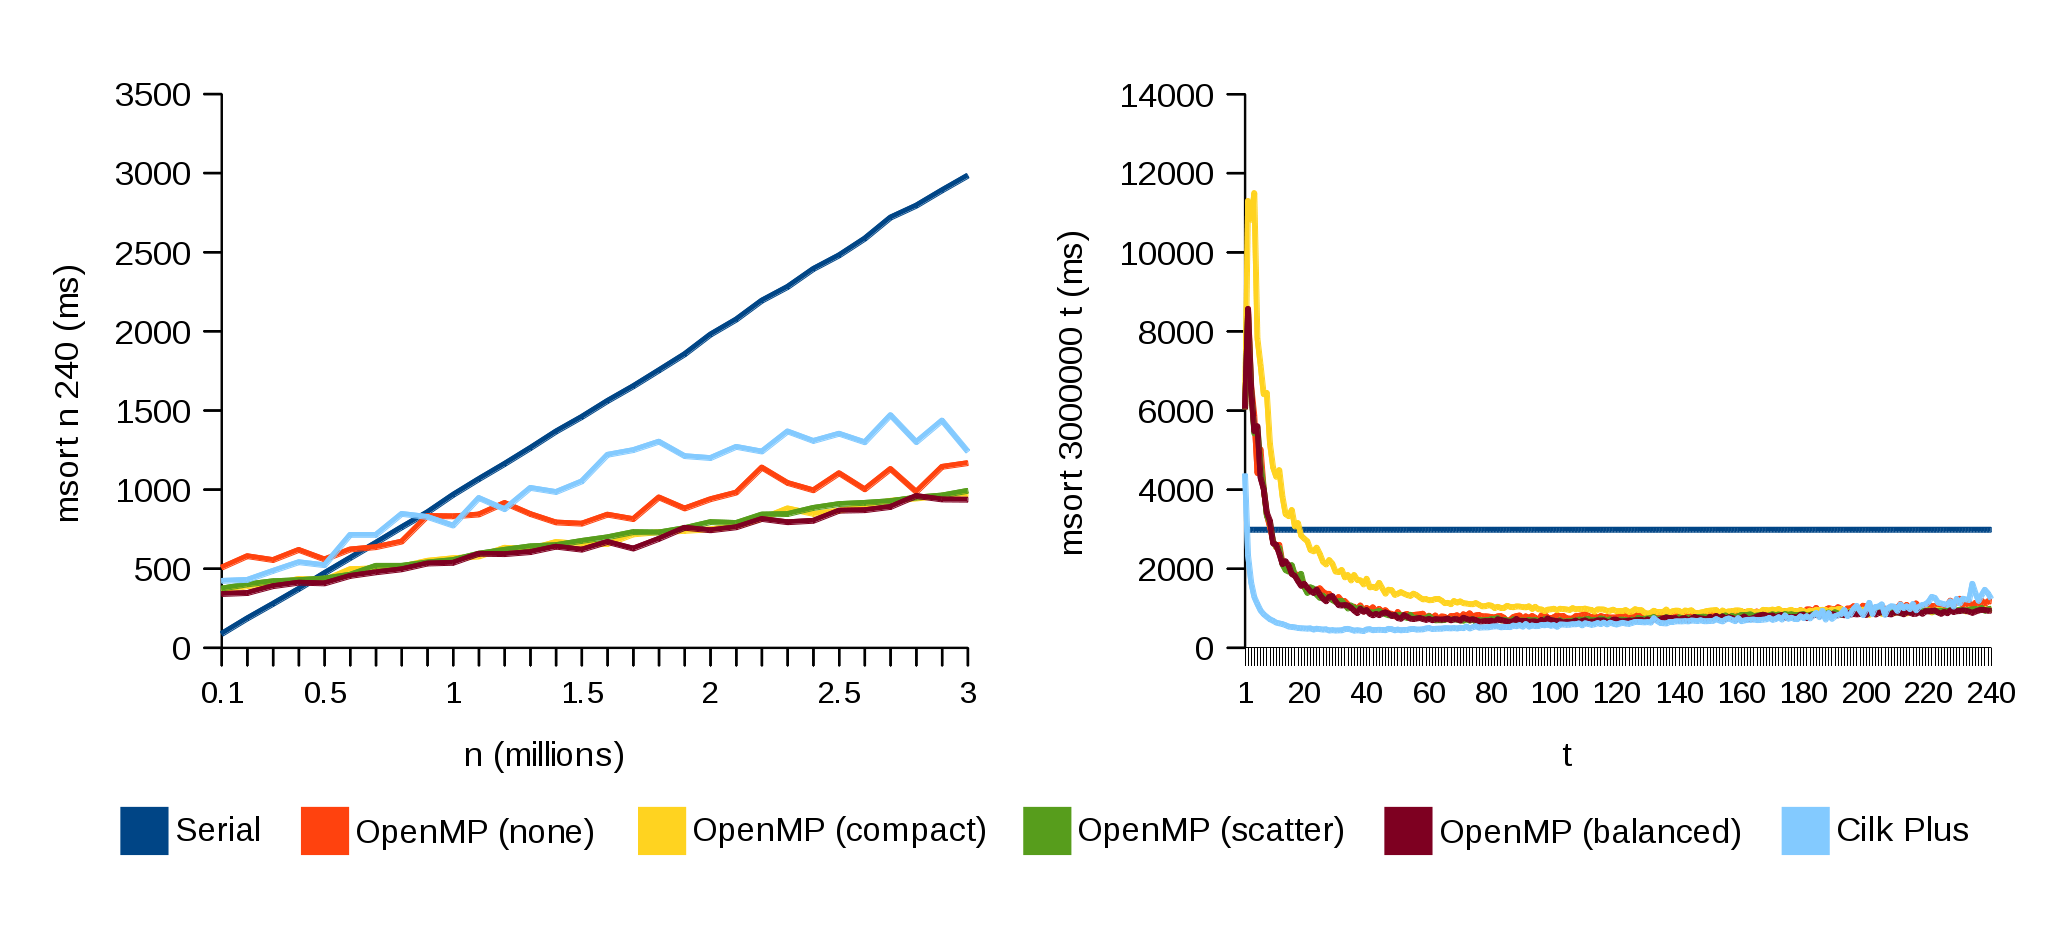
\includegraphics[width=\linewidth]{../../charts/mic/msort_time}
	\caption{Execution time (milliseconds) of the merge sort benchmark on the Xeon Phi.}
	\label{Fig:msortmictime}
\end{figure}
\noindent
\begin{figure}[t!]
	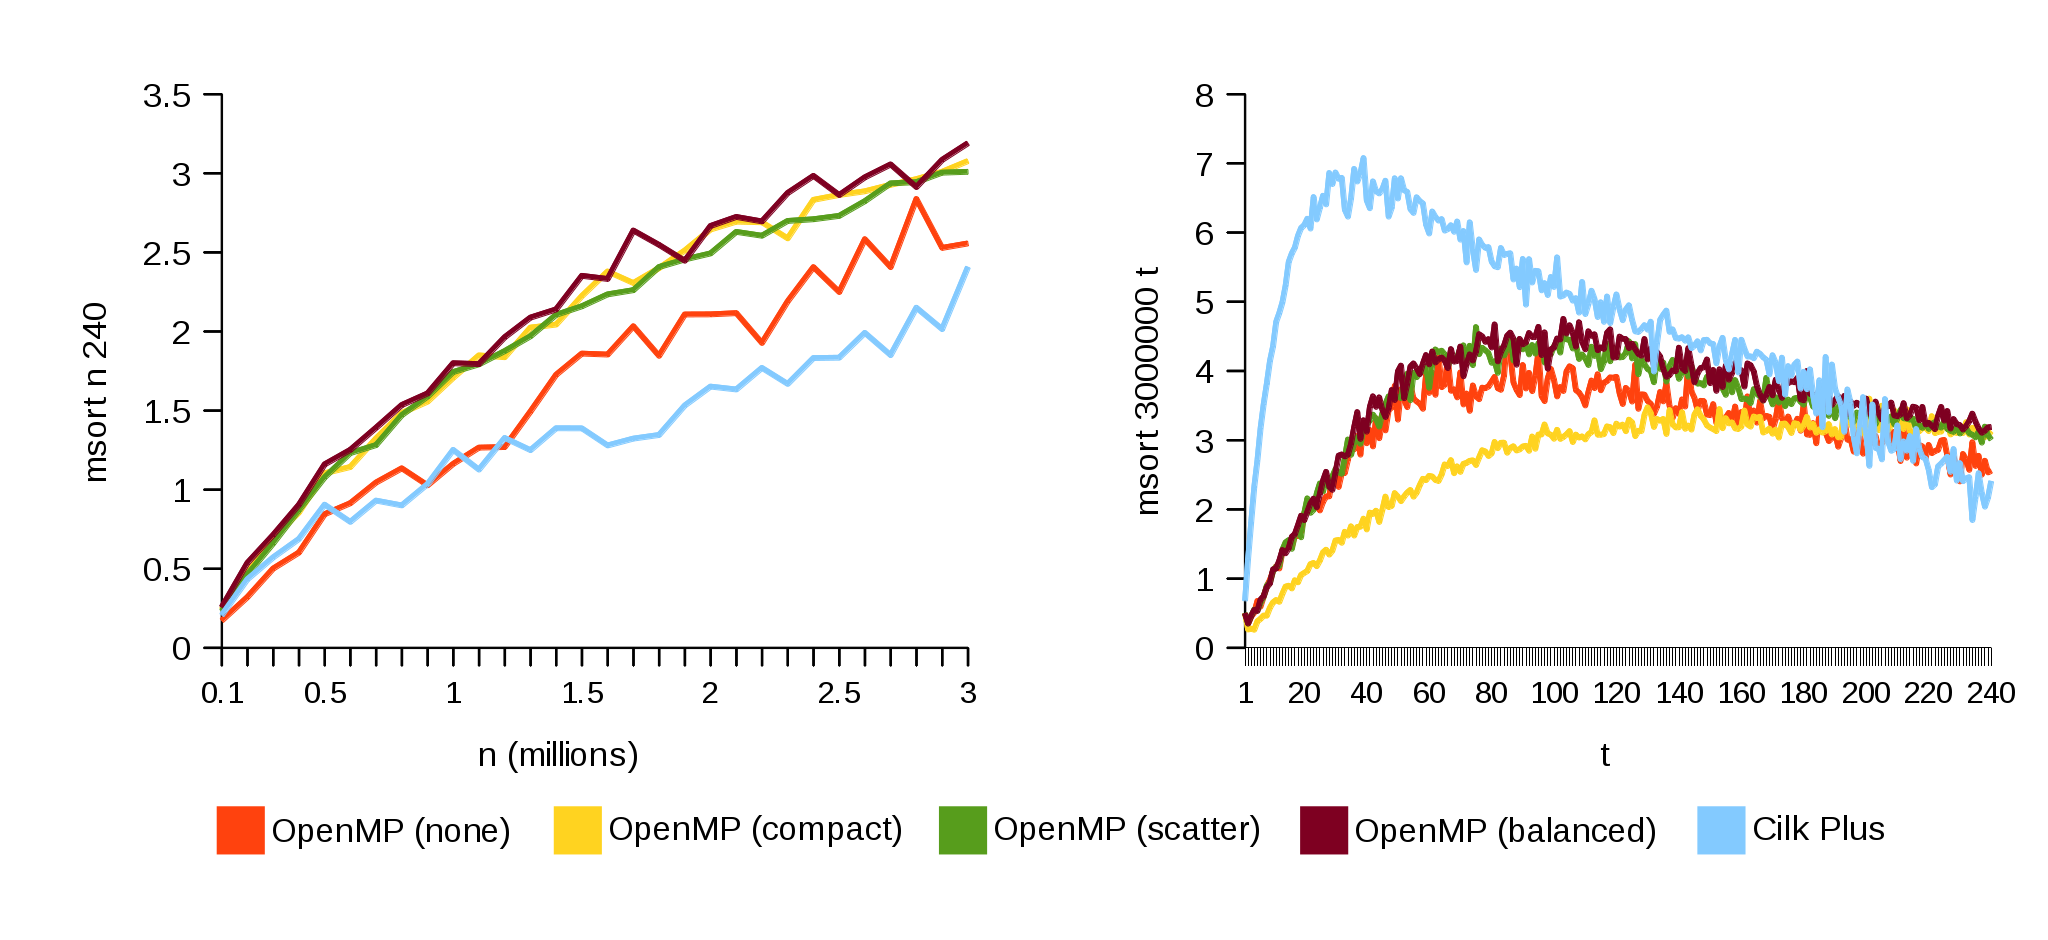
\includegraphics[width=\linewidth]{../../charts/mic/msort_speedup}
	\caption{Speedup of the merge sort benchmark on the Xeon Phi.}
	\label{Fig:msortmicspeedup}
\end{figure}

However, Figure \ref{Fig:msortmicspeedup} (right) shows why this interpretation of the data may be misleading. When fewer threads are available than the total possible, Cilk Plus outperforms OpenMP by a significant margin. It achieves seven times speedup at around \(t=40\), before entering a steep and steady decline when more threads are made available. This is perfectly consistent with the results presented by Tousimojarad and Vanderbauwhede\cite{Tousimojarad14}, who performed a similar test on the Xeon Phi. Using a cut-off value, they found that Cilk Plus achieved a 12 times speedup when sorting 80 million integers. This occurred when around 64-threads were used, followed by the same decline present in the data produced for this project. They also observed that OpenMP outperforms Cilk Plus when almost all of the Xeon Phi's threads are utilised. However, they found the decline to be much shallower, and the difference with OpenMP to be smaller at all values of \(t\). The difference in the value of \(t\) when the peak occurred, as well as in the shallower gradient of the decline, may be due to their use of a cut-off value  equal to one 2048\textsuperscript{th} of the input array size. An additional feature of Figure \ref{Fig:msortmicspeedup} (right) is the clear underperformance of compact thread affinity for most values of \(t\). This may again be due to OpenMP attempting to use all threads in each core before starting threads on the next. This would be consistent with the trend present in the data, where the difference in thread affinity narrows as the Xeon Phi approaches full thread utilisation. At a higher resolution than presented here, the merge sort benchmark produced a noticeable pattern as \(n\) increased. The nature of the pattern did not indicate that it was caused by noise, but further investigation, conducted by increasing the test range to include points at which individual core caches would be filled, and more powers of two, did not produce an adequate explanation of the phenomenon. Reducing the increment to 25,000 produced even higher resolution data, in which the patterns were still present, but presented no additional clues that would help identify their origin. One possibility is that the pseudo-random number generation used to fill the arrays was generating the same set of numbers in a pattern, causing different trials to have similar execution times due to similar ``random" input arrays. Unfortunately, time constraints did not permit the exploration of this possibility.

Figure \ref{Fig:msortmicheatmap} shows the heatmaps produced by performing the merge sort benchmark for every combination of \(n\) and \(t\). Using no thread affinity with OpenMP again introduces greater variation than alternative strategies, but one of the most prominent features of the heatmaps produced from the Xeon Phi data is the yellow area on the Cilk Plus chart. This is the result of the performance decline discussed above, and affects a large range of input combinations. The decline is so severe that just a few threads are able to sort much larger arrays than when 240 threads are used, indicated by the large area of green. The overhead that may have caused the lower part of all heatmaps on the host machine to be shown as blue is not as clear here.
\noindent
\begin{figure}[t!]
	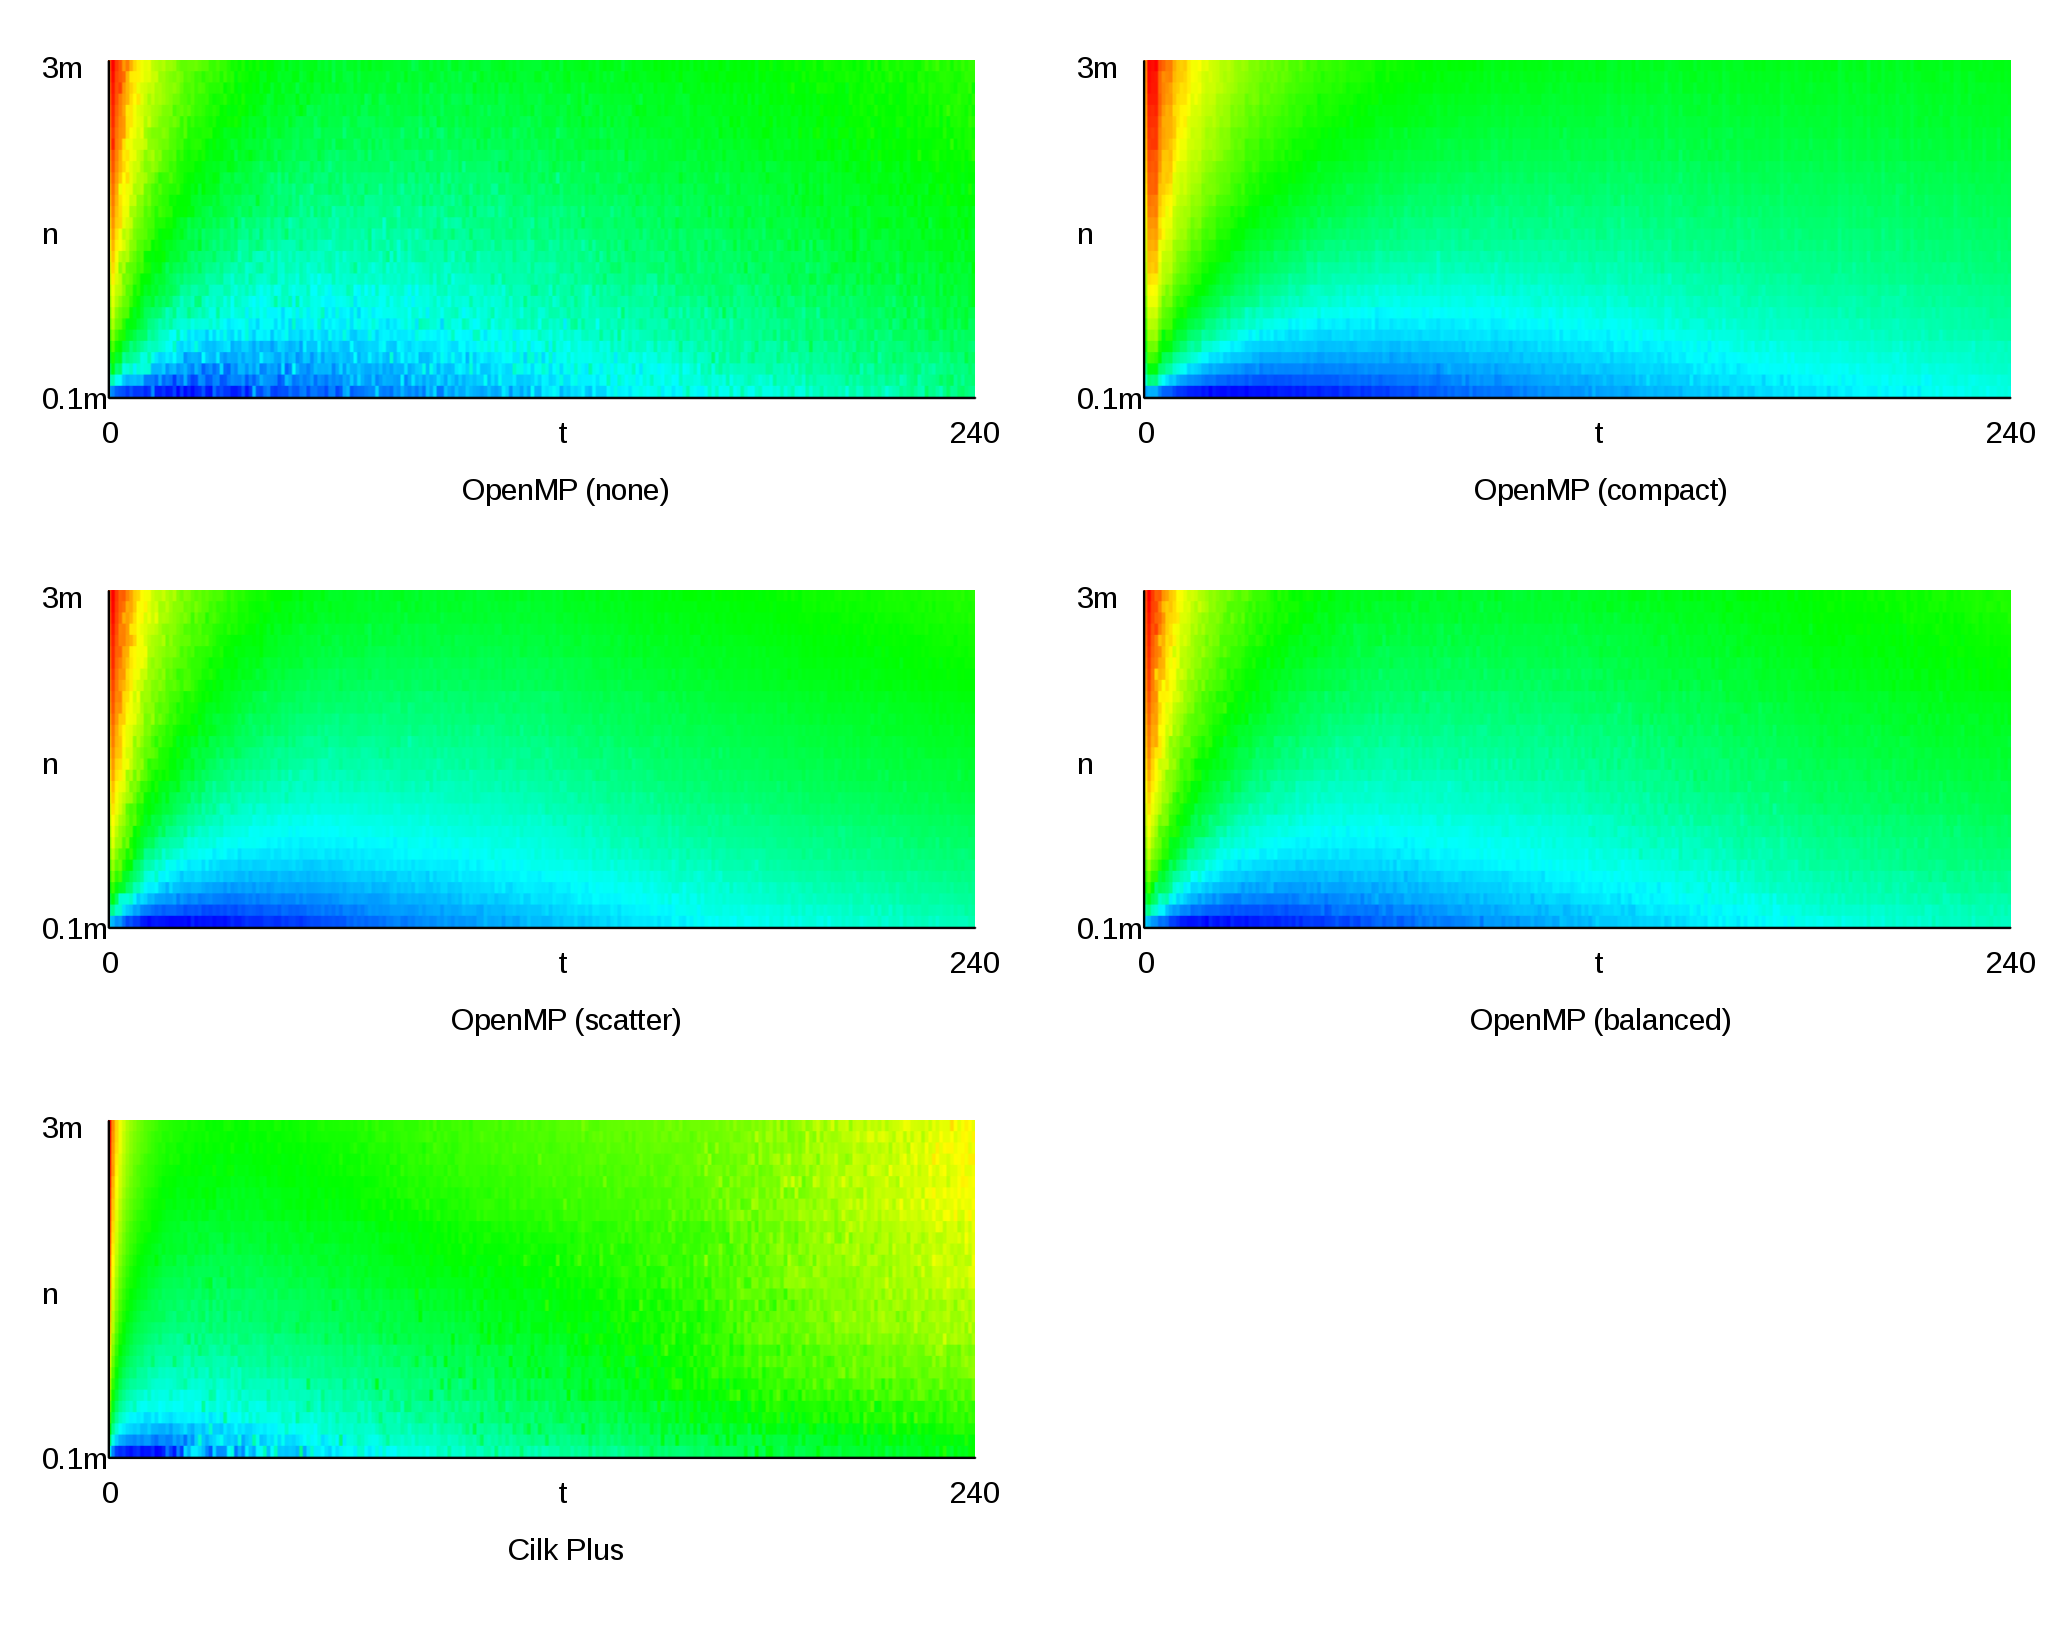
\includegraphics[width=\linewidth]{../../heatmaps/mic/msort}
	\caption{Heatmaps showing performance spread of merge sort benchmark for different combinations of n and t on the Xeon Phi.}
	\label{Fig:msortmicheatmap}
\end{figure}

\subsection{Powers-of-two} \label{Sec:evalmsortpowers}

The powers-of-two merge sort benchmark used the same program as Section \ref{Sec:evalmsortstandard}; only the values of \(n\) were changed. Instead of increments of 100,000, the size of \(n\) was increased exponentially. For each trial, \(n=2\textsuperscript{e}\) where \(e \in [10,22]\), resulting in 12 trials for each value of \(t\). Each array used therefore had a size equal to a power of two, allowing it to be split perfectly until the resulting array had only one element. This presents the best-case load-balancing scenario for a program executing the merge sort benchmark.
\noindent
\begin{figure}[t!]
	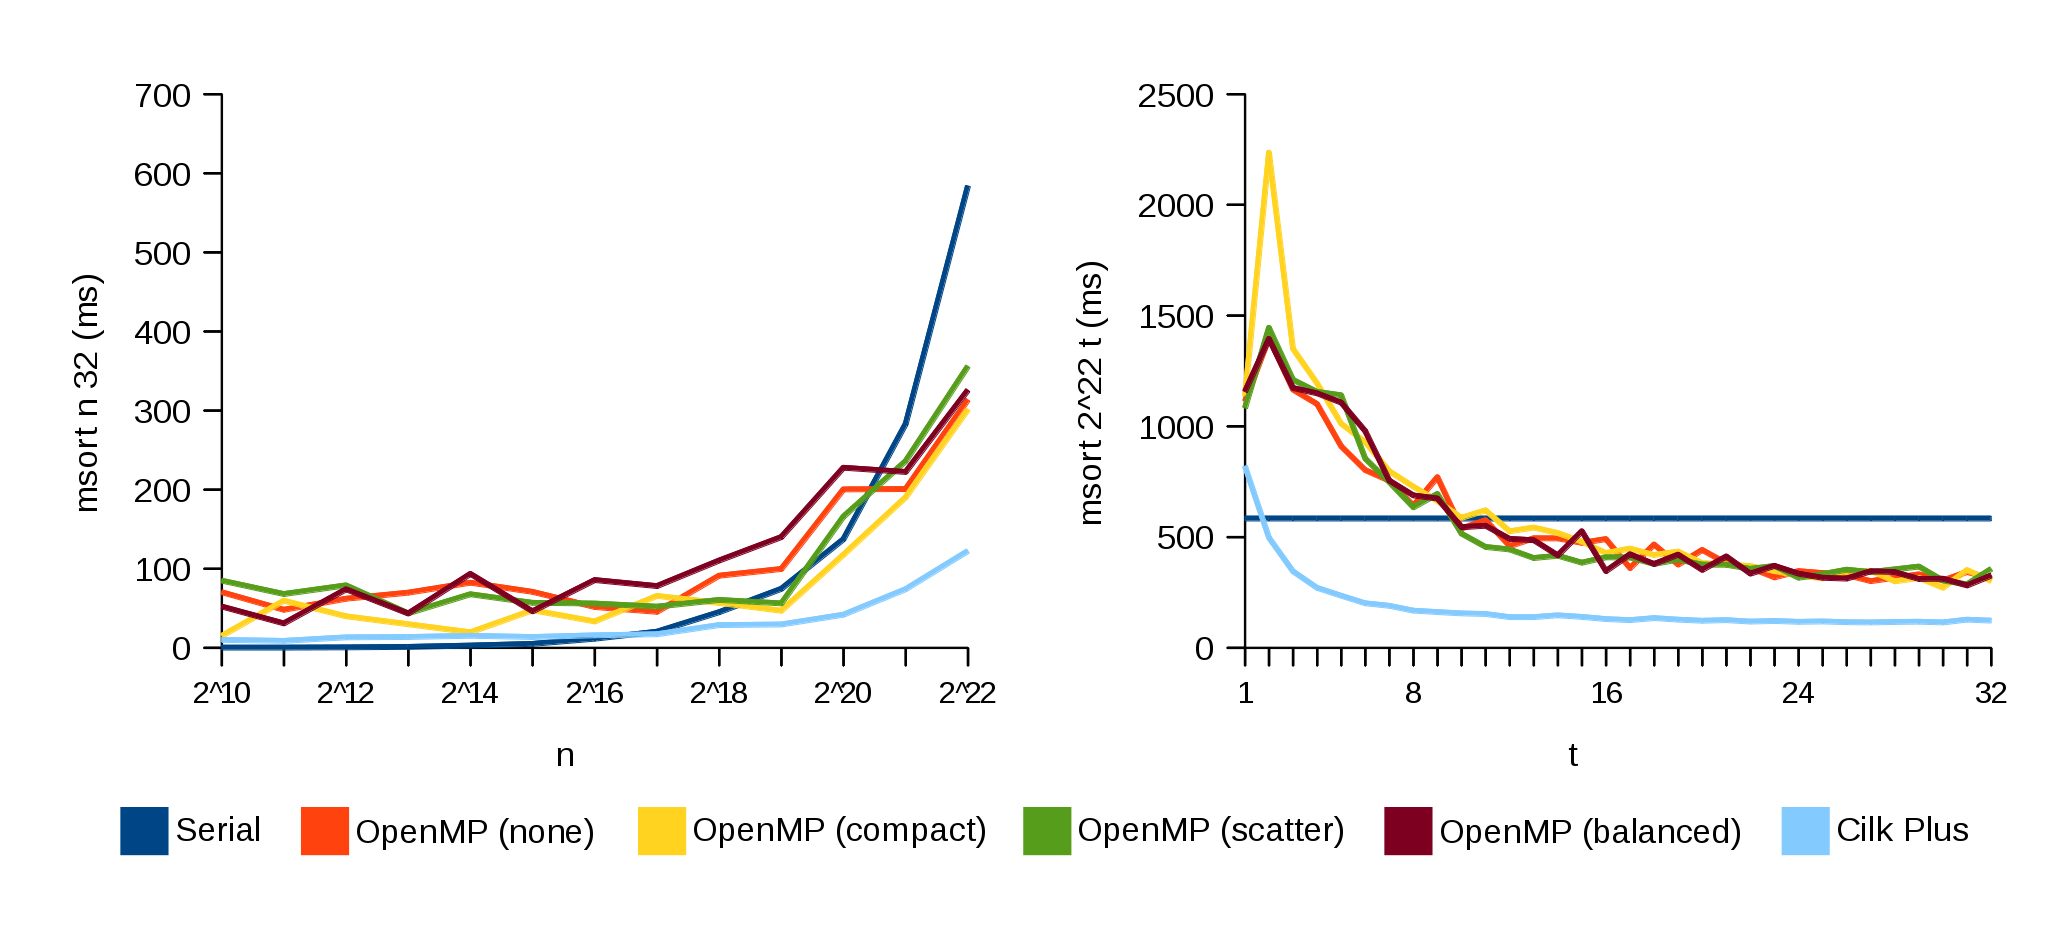
\includegraphics[width=\linewidth]{../../charts/intel64/msort_powers_time}
	\caption{Execution time (milliseconds) of the powers-of-two merge sort benchmark on the host machine.}
	\label{Fig:msortpowershosttime}
\end{figure}
\noindent
\begin{figure}[t!]
	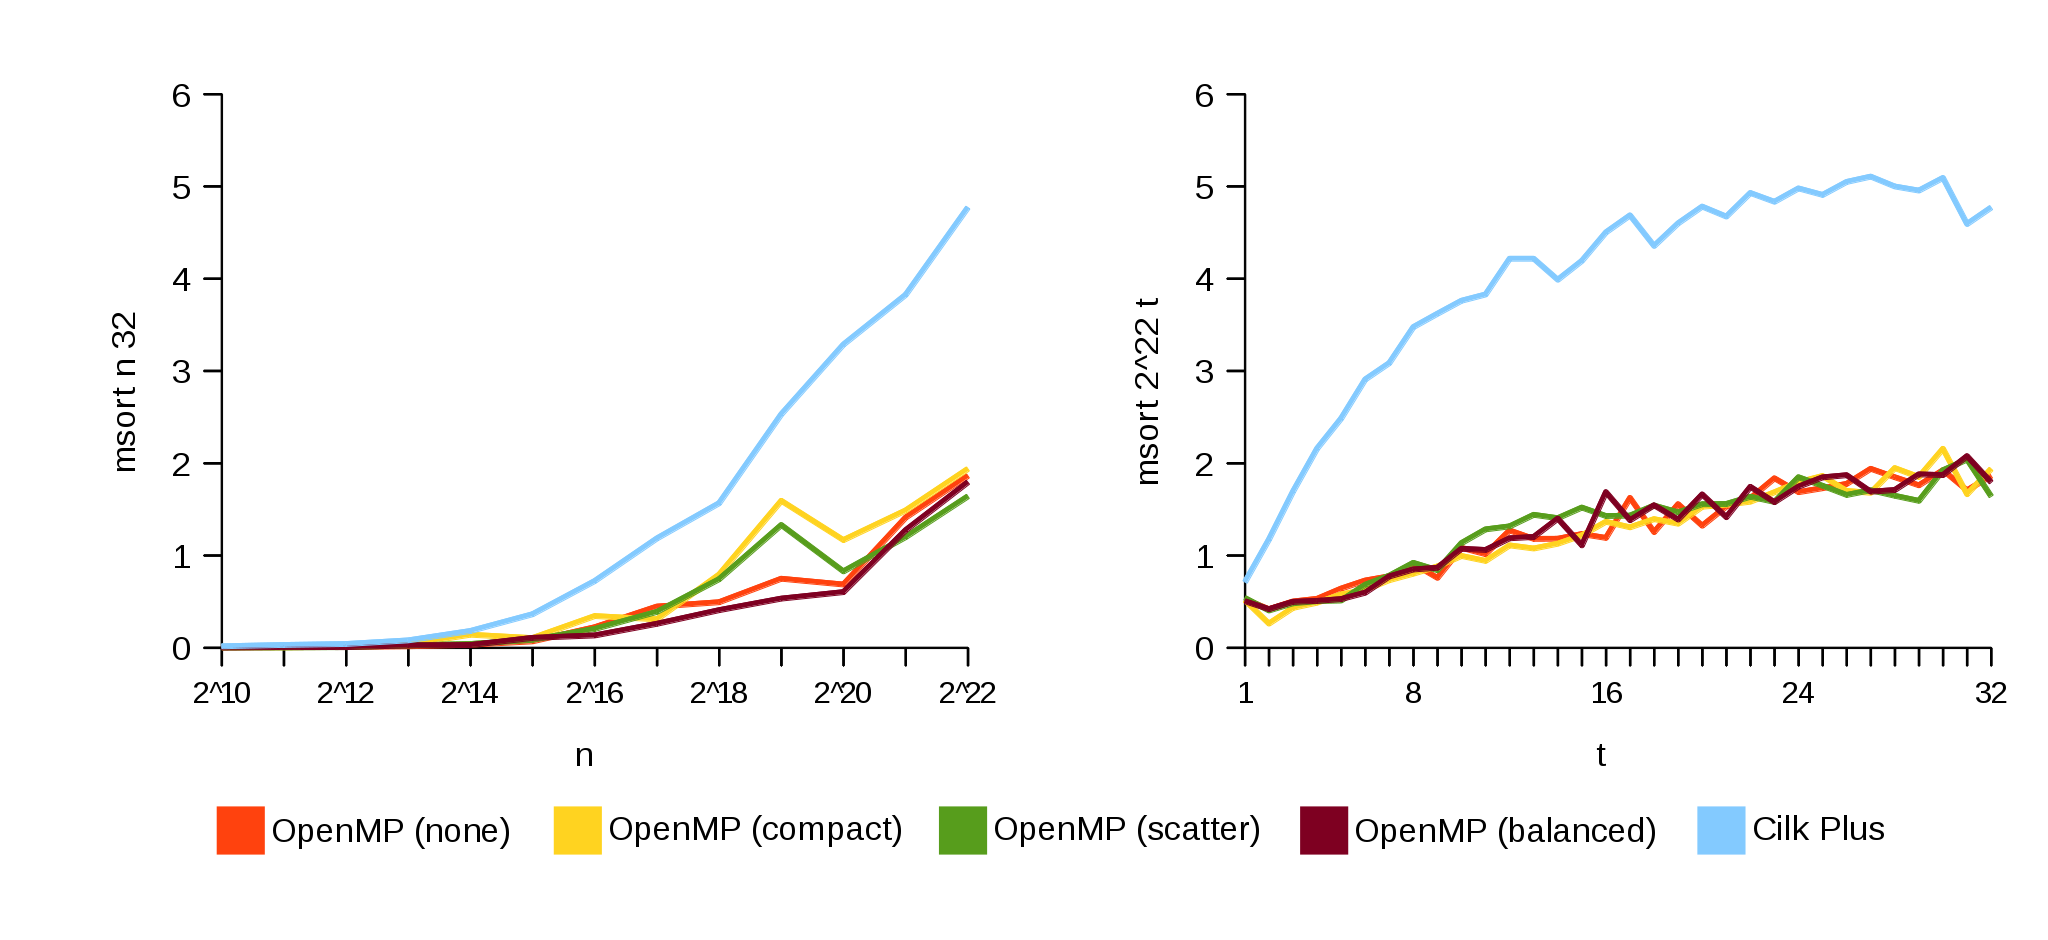
\includegraphics[width=\linewidth]{../../charts/intel64/msort_powers_speedup}
	\caption{Speedup of the powers-of-two merge sort benchmark on the host machine.}
	\label{Fig:msortpowershostspeedup}
\end{figure}

\subsubsection{Host}

As expected, the serial version shows an exponential increase in execution time as \(e\) is incremented in Figure \ref{Fig:msortpowershosttime} (left). OpenMP and Cilk Plus likewise show a significant increase for larger values of \(e\), but Figure \ref{Fig:msortpowershostspeedup} (left) shows how this translates into improved performance of the serial trials. When \(n=2\textsuperscript{22}\), OpenMP achieves almost double the performance of the serial version, and Cilk Plus sees a five times improvement. For lower values of \(e\), any parallel gains are lost in the overhead caused by parallelisation, although it should be noted that the overhead induced by Cilk Plus appears to be much lower. Figure \ref{Fig:msortpowershosttime} (right) show the results obtained by running the merge sort benchmark with an input array of size 2\textsuperscript{22} with 32 threads on the host machine. Many of the same features apparent in the standard version are also present here, such as the spike for OpenMP compact affinity, and the consistently lower execution times achieved by Cilk Plus, resulting in a plateau of around five times speedup over the serial version in Figure \ref{Fig:msortpowershostspeedup} (right) after 24 threads are used. Another feature also present in the results for the standard version that also appears here is slight wavering of the otherwise consistent trend when 16 thread are used, possibly due to the scheduler having to pass tasks between CPUs across the QPI.
\noindent
\begin{figure}[t!]
	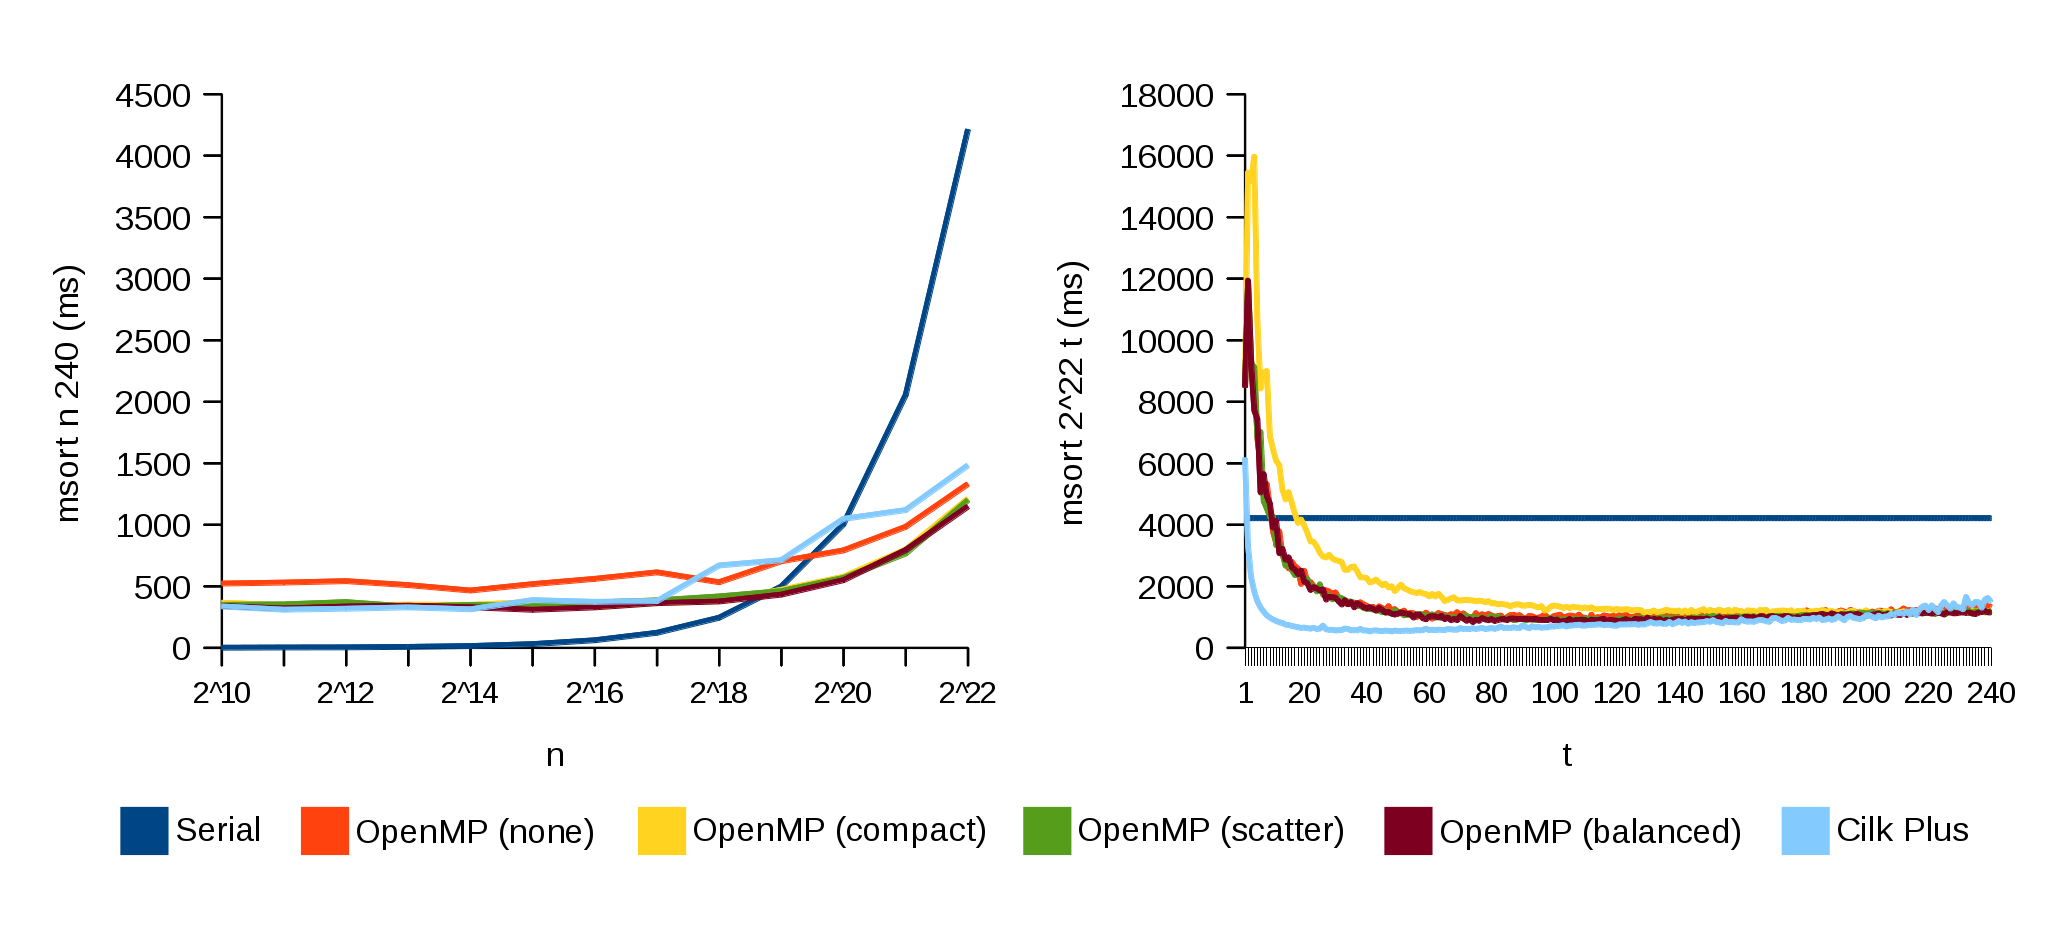
\includegraphics[width=\linewidth]{../../charts/mic/msort_powers_time}
	\caption{Execution time (milliseconds) of the powers-of-two merge sort benchmark on the Xeon Phi.}
	\label{Fig:msortpowersmictime}
\end{figure}
\noindent
\begin{figure}[t!]
	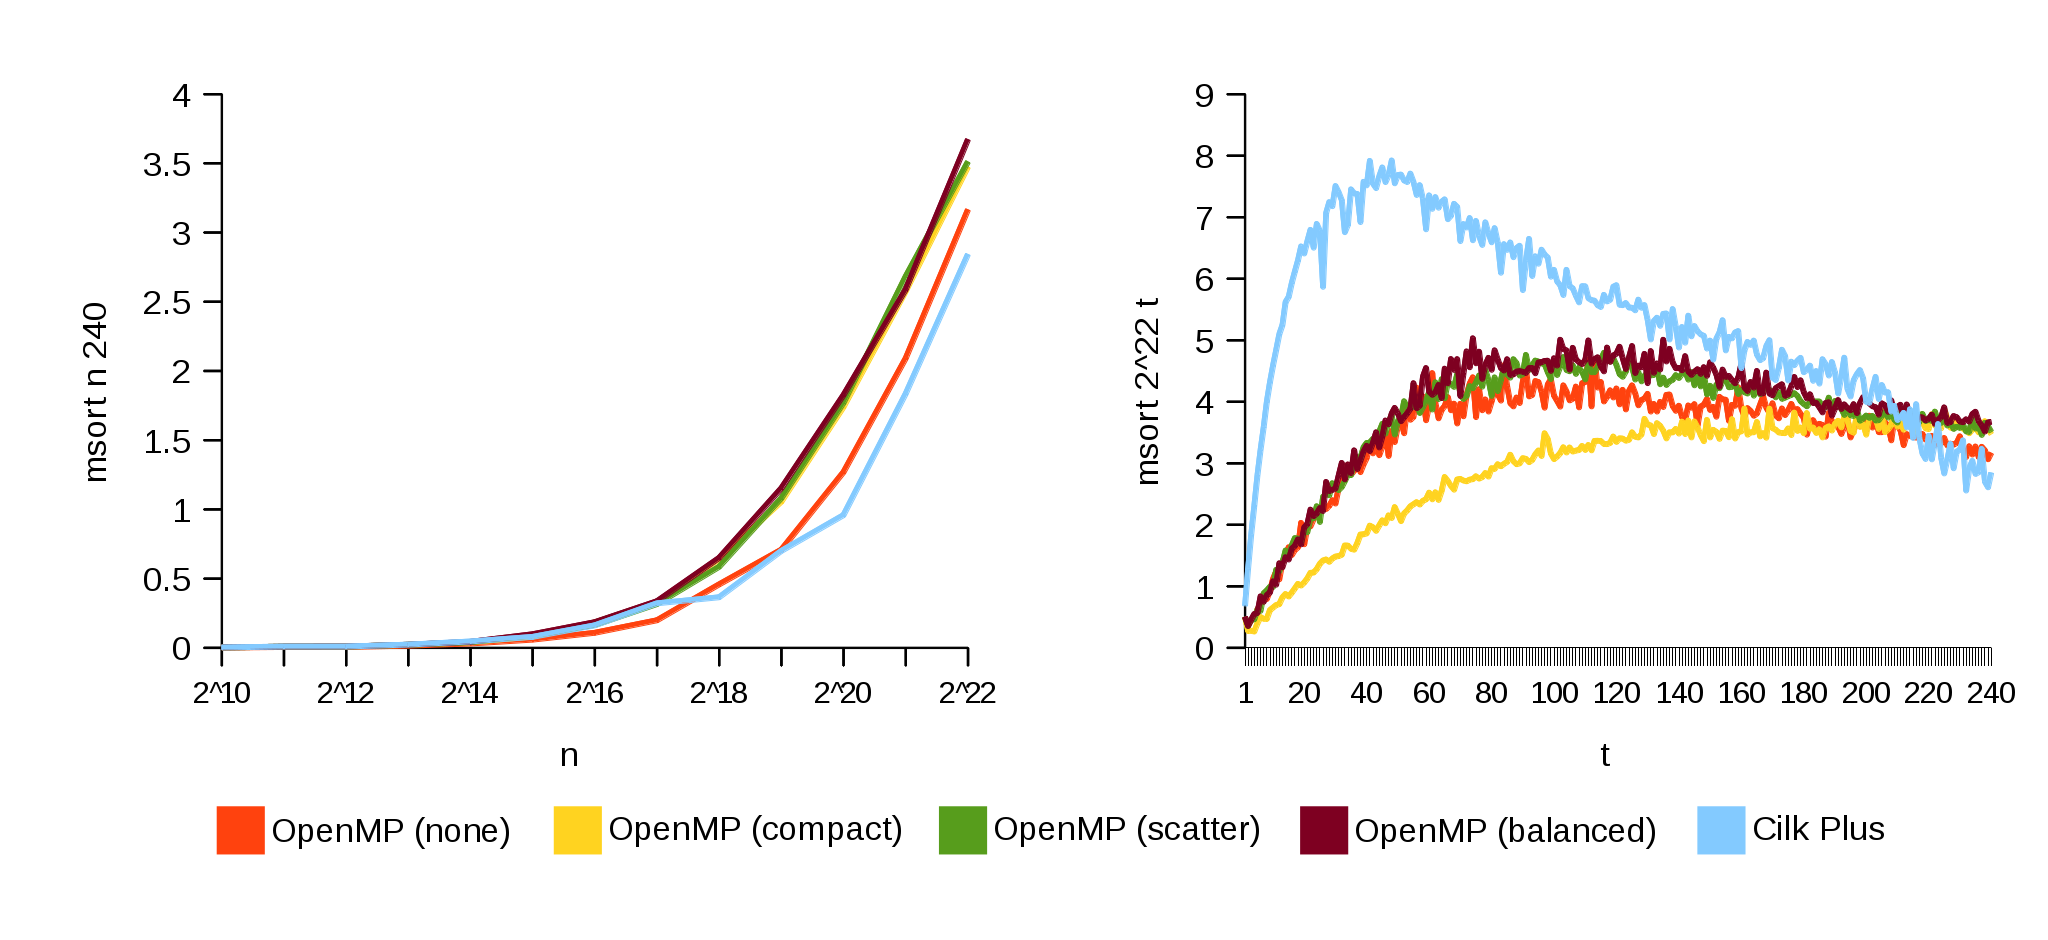
\includegraphics[width=\linewidth]{../../charts/mic/msort_powers_speedup}
	\caption{Speedup of the powers-of-two merge sort benchmark on the Xeon Phi.}
	\label{Fig:msortpowersmicspeedup}
\end{figure}

\subsubsection{Xeon Phi}

Figure \ref{Fig:msortpowersmictime} (left) shows the results of performing the same trials on the Xeon Phi using 240 threads. The same exponential serial pattern is visible, as are the accelerating increases in execution time for all parallel versions. Also visible here is the shallower angle of this incline than can be seen on the host machine, as well as the higher parallel overhead for low values of \(n\). As in the results for the standard version, Cilk Plus performs worse than OpenMP for higher values of \(n\).

Figure \ref{Fig:msortpowersmictime} (right), however, shows that the slight variations in the host machine data when 12 or 16 threads are used disappear, further suggesting that they were caused by the need for the Xeon processors to communicate via the motherboard, rather than the internal ring interconnect featured in the Xeon Phi. One may also expect these variations to appear if the same Xeon Phi trials were conducted in offload mode, where two cards would need to communicate via the PCI-E bus when the number of available threads exceeded the capabilities of a single device.

\subsubsection{Comparison}

The powers-of-two benchmark did not produce many notable differences with the standard version. More consistent results on the host machine were seen, as was the disappearance of the patterns in the data that had been observed in the results produced by the standard version on the Xeon Phi. This may indicate that the patterns were caused by some particular aspect of the hardware that has not been appreciated, such as memory bandwidth being saturated by uneven input data at regular intervals. The superior load-balancing capabilities of Cilk Plus reported in the literature do not seem to result in any difference in the relative performance of Cilk Plus and OpenMP between the standard version and the powers-of-two benchmarks. The strong similarities with the standard version may help to explain why the powers-of-two benchmark does not appear in the literature.

\section{N-Queens} \label{Sec:evalnqueens}

Two versions of N-Queens were created for this project. The standard version creates fine-grained tasks, while the cut-off version introduces a cut-off value \(c\) intended to increase the coarseness of the tasks generated and improve performance. Heatmaps are omitted from the evaluation of N-Queens because the wide range of execution times in the results reduced their usefulness.

\subsection{Standard Version} \label{Sec:evalnqueensstandard}

This section evaluates the performance of the standard version of N-Queens, without cut-off, on the host machine and Xeon Phi. Some attention is paid to the effectiveness of Cilk Plus' parallel for-loop feature and how it compares in performance to the OpenMP alternative involving manual task creation.

\subsubsection{Host}
Figure \ref{Fig:nqueenshosttime} (left) shows the performance of the N-Queens benchmark when executed on the host machine. Note that the execution times vary so widely in the results that a logarithmic scale has been used to make the differences between the serial, OpenMP and Cilk Plus implementations more apparent. An interesting feature of the results for the serial trials is that the time taken to calculate all valid solutions to the puzzle for values of \(n<8\) does not register on the chart, while later results increase logarithmically. This is not totally unexpected, since the number of solutions to the N-Queens puzzle increases rapidly for larger values of \(n\), as do the number of possible board states that must be checked. In comparison, the parallel versions all feature the same overhead, around 100 ms for 32 threads, as appeared in the other benchmarks. At around \(n=10\), the parallel versions enter the same logarithmic incline as the serial version, but always take longer to complete. Figure \ref{Fig:nqueenshostspeedup} (left) shows this more clearly, with Cilk Plus again outperforming OpenMP, but never achieving a speedup of more than 0.6. This is the result of a steep incline in speedup, however, and it may be that this trend continues until true parallel speedup is achieved as some higher value of \(n\). The workload of \(n=13\) is greater than presented by some other authors, such as Blumofe \textit{et al.}\cite{Blumofe95} who used \(n=15\) in 1995. In later papers, even larger input values are used dependent upon the hardware being tested, such as Leiserson and Plaat\cite{Leiserson97} who used a value of \(n=22\) in 1997, and Rehr and Vinter\cite{Vinter08} who placed 18 queens on a single Cell processor in 2008. The poor speedup demonstrated in this benchmark may be due to 13 queens simply not being enough for the benefits of parallelisation to become apparent on two Xeon processors. Counter to this, however, is that OpenMP actually shows a drop in performance for larger values of \(n\).
\noindent
\begin{figure}[t!]
	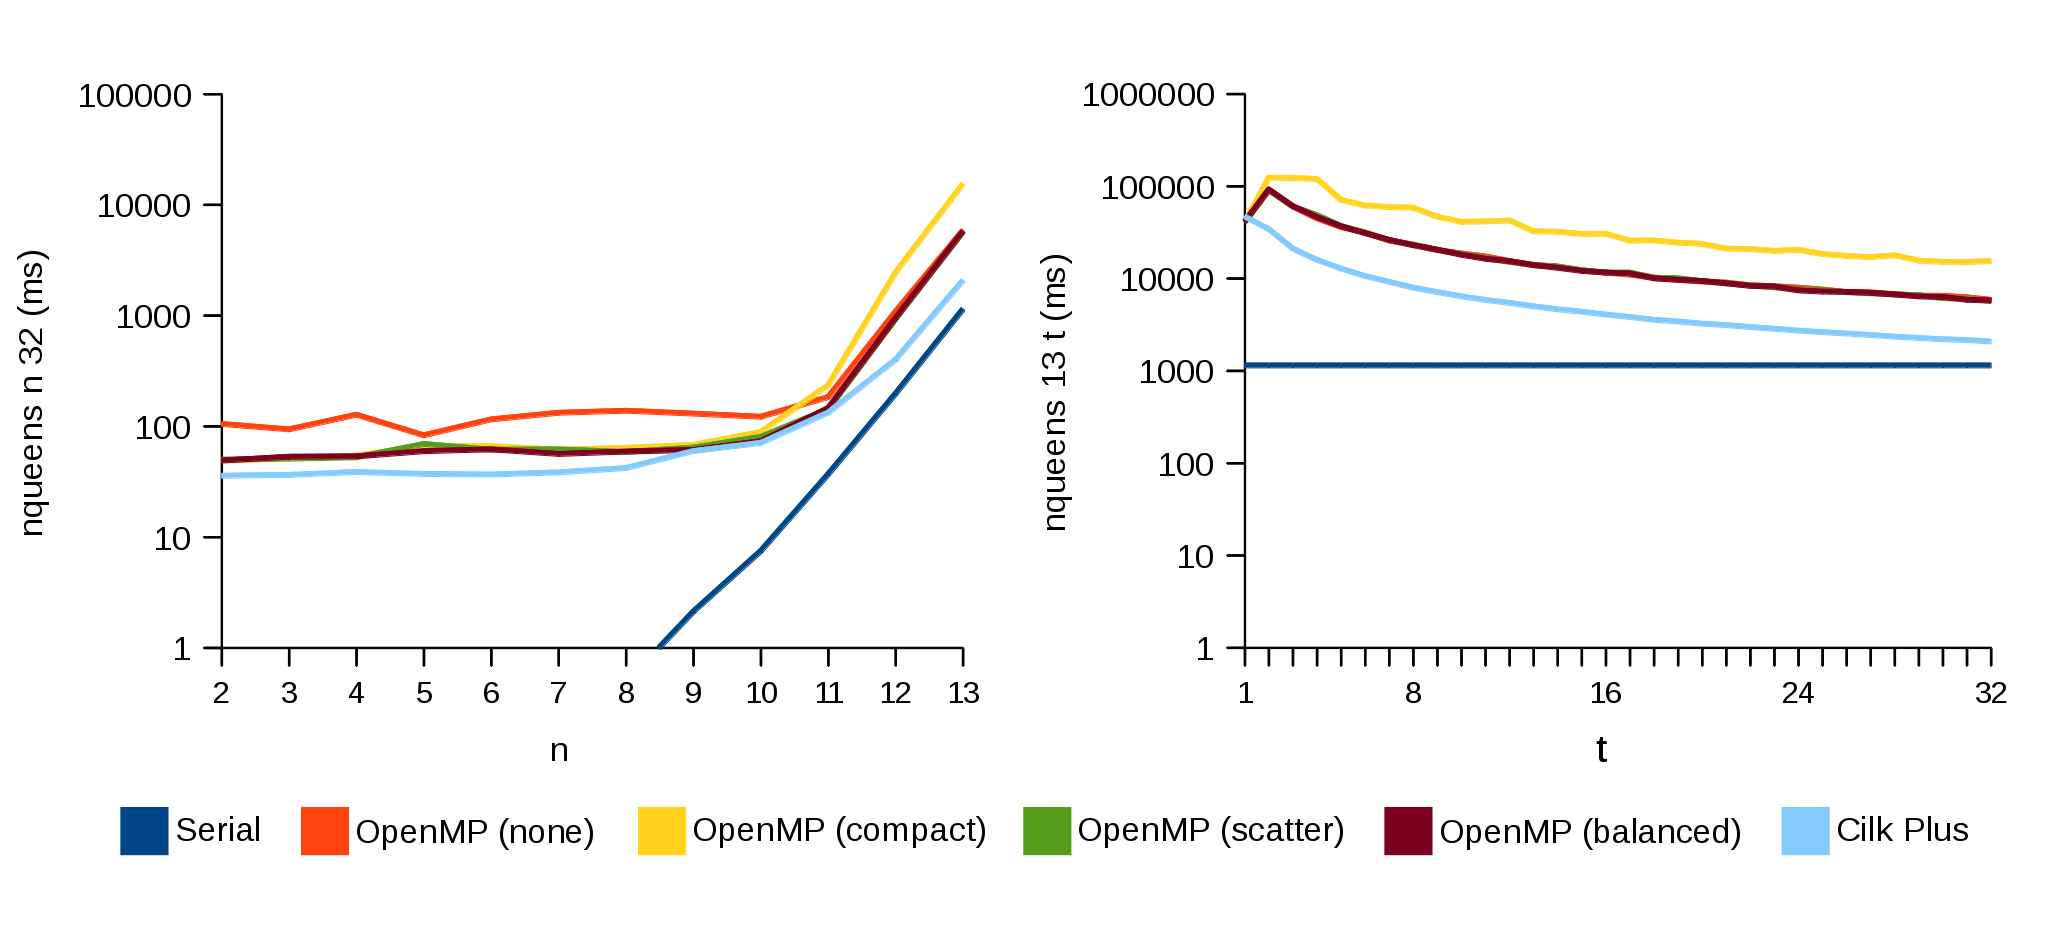
\includegraphics[width=\linewidth]{../../charts/intel64/nqueens_time}
	\caption{Execution time (milliseconds) of the N-Queens benchmark on the host machine.}
	\label{Fig:nqueenshosttime}
\end{figure}
\noindent
\begin{figure}[t!]
	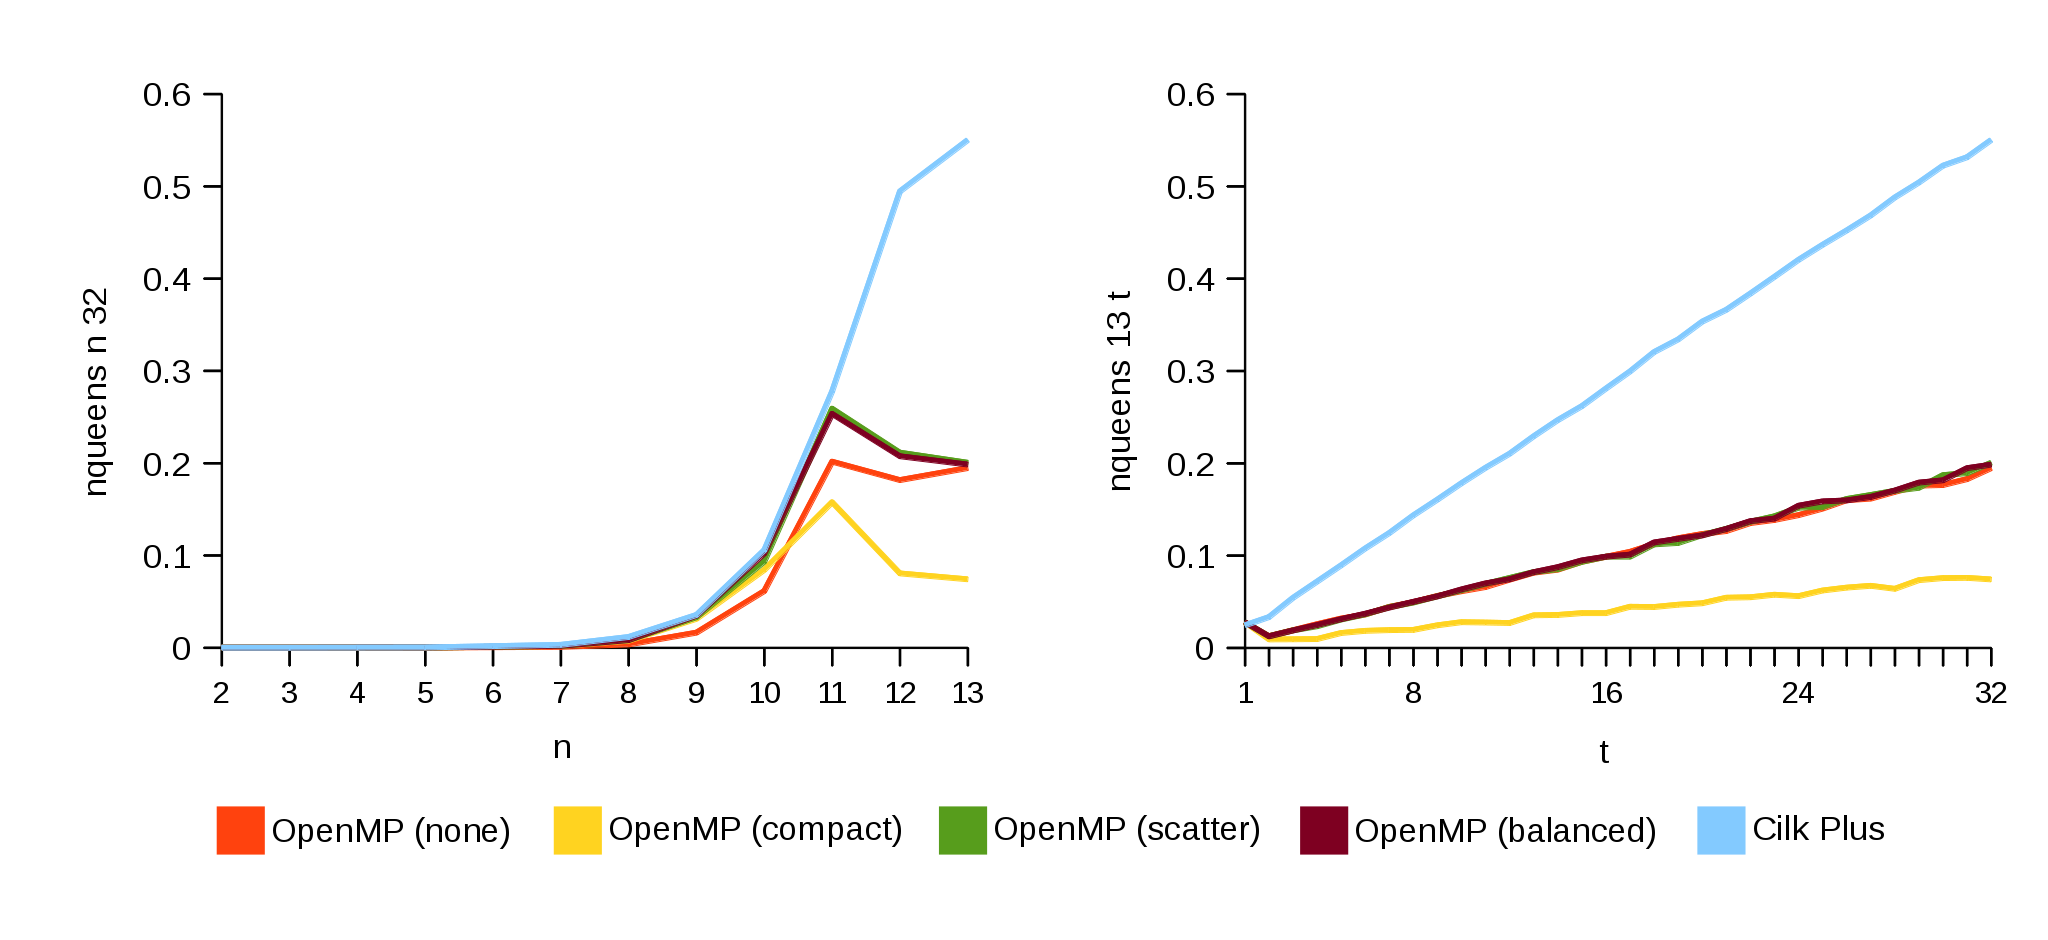
\includegraphics[width=\linewidth]{../../charts/intel64/nqueens_speedup}
	\caption{Speedup of the N-Queens benchmark on the host machine.}
	\label{Fig:nqueenshostspeedup}
\end{figure}

Figure \ref{Fig:nqueenshosttime} (right) shows the performance of the N-Queens benchmark when \(n=13\) and the number of available threads is increased. Cilk Plus and OpenMP both see continued benefits as the number of threads increases, and Figure \ref{Fig:nqueenshostspeedup} (right) shows that this trend continues linearly for all implementations throughout the trial range. Cilk Plus consistently outperformed OpenMP, however, and this may be due to additional overhead caused by the manual spawning of tasks in the absence of a specialised task-parallel for-loop like Cilk's \verb!cilk_for!.

\subsubsection{Xeon Phi}

Figure \ref{Fig:nqueensmictime} (left) shows the same trials conducted on the Xeon Phi, using 240 threads. As before, the scale is logarithmic due to the enormous difference in execution time between trials. Similar to other benchmarks, the Xeon Phi performed worse than the host machine, demonstrated by the serial implementation only appearing on the chart after \(n=7\). Furthermore, the parallel versions show the same increased overhead over the Xeon that was detected in the other benchmarks. However, on the Xeon Phi, both Cilk Plus and OpenMP achieve speedup within the trial range. Figure \ref{Fig:nqueensmicspeedup} (right) shows that the parallel implementations both perform better than the serial version when placing 11 queens, but that Cilk Plus enters a much steeper performance incline after this. For the highest value of \(n\), Cilk Plus achieves speedup of around 12 times, while OpenMP only achieves half of this. This difference with the results produced by the host machine may be due to the lower clock rate of the Xeon Phi making it easier for the parallel versions to achieve positive speedup. Indeed, Figures \ref{Fig:nqueensmictime} (right) and \ref{Fig:nqueensmicspeedup} (right) show Cilk Plus achieving around a 16 times speedup over the serial implementation when \(n=13\) and between 100 and 120 threads are used -- only half of the Xeon Phi's maximum. This is identical to the trend observed by Lima \textit{et al.}\cite{Lima13}; performance peaked at around 100-120 threads for both OpenMP and Cilk Plus, but they saw almost an order-of-magnitude better speedup than presented here. This may be due to their use of a global variable to count the number of valid solutions, rather than the serial array sum that was used in this project's implementation of N-Queens. The difference may also be caused by their use of a larger input value, \(n=17\).
\noindent
\begin{figure}[t!]
	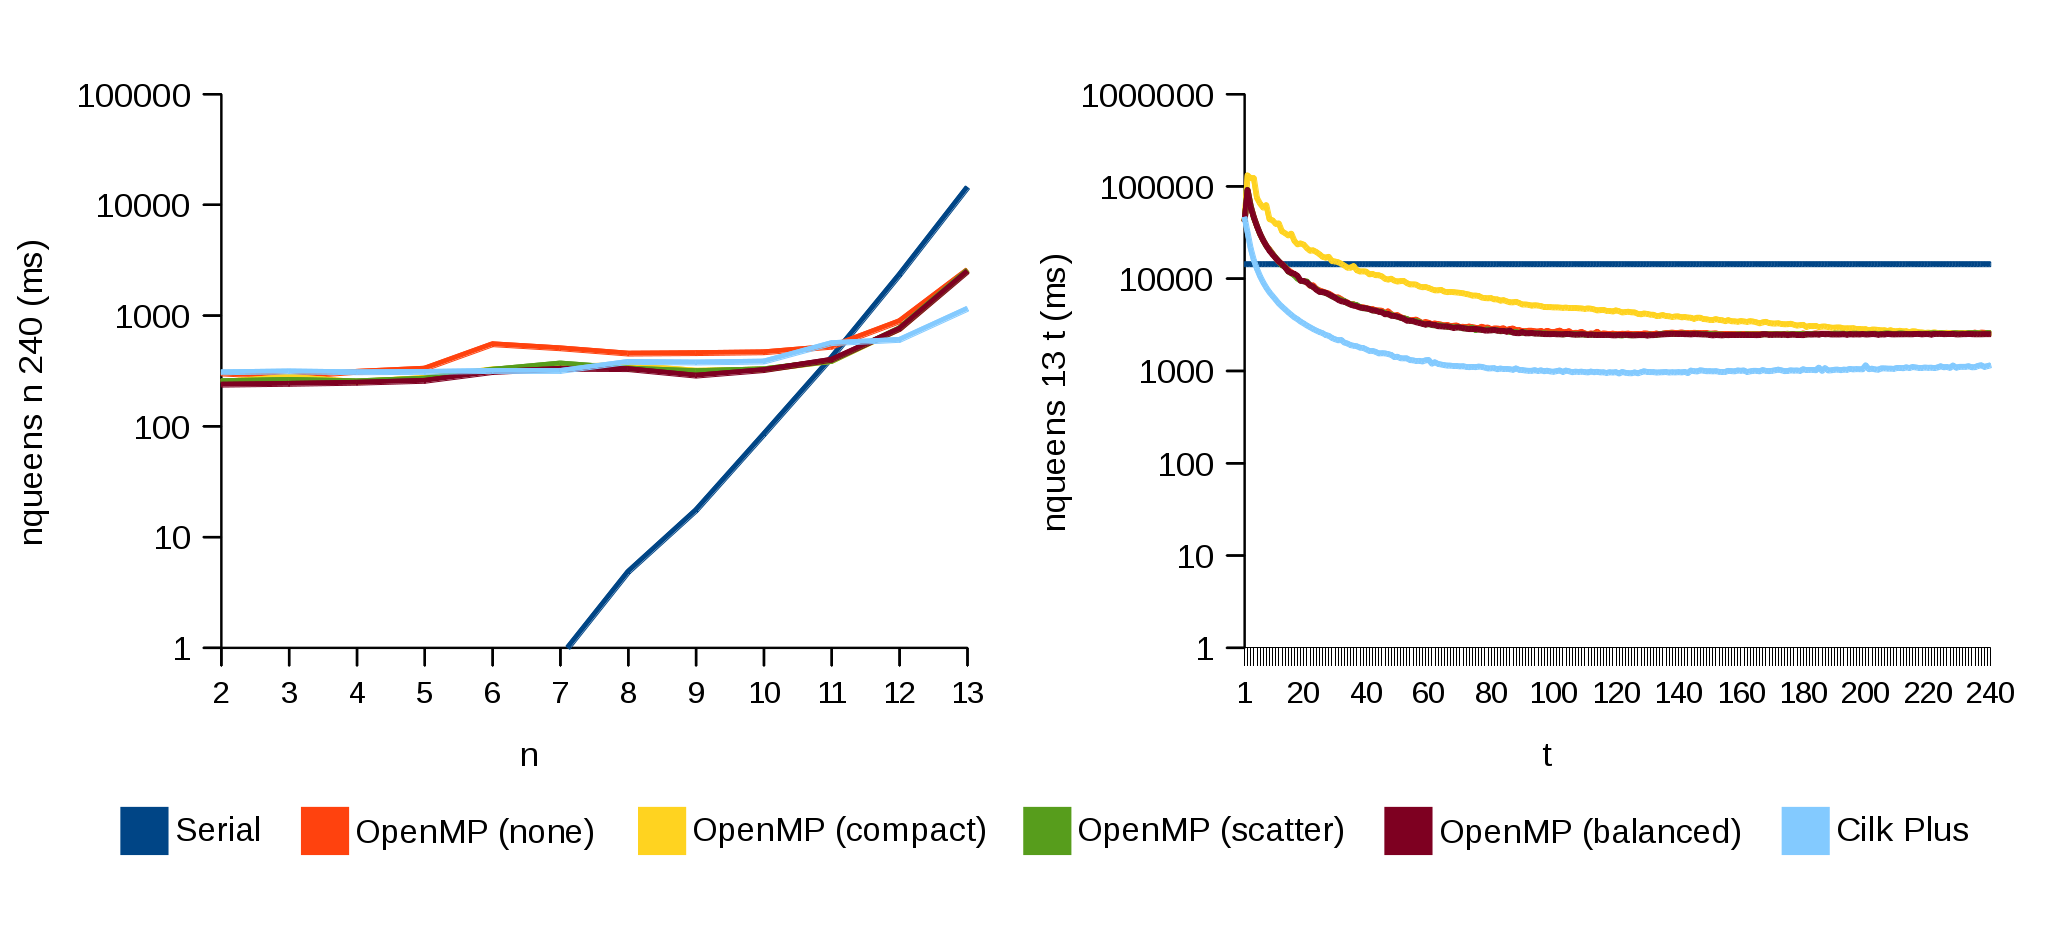
\includegraphics[width=\linewidth]{../../charts/mic/nqueens_time}
	\caption{Execution time (milliseconds) of the N-Queens benchmark on the Xeon Phi.}
	\label{Fig:nqueensmictime}
\end{figure}
\noindent
\begin{figure}[t!]
	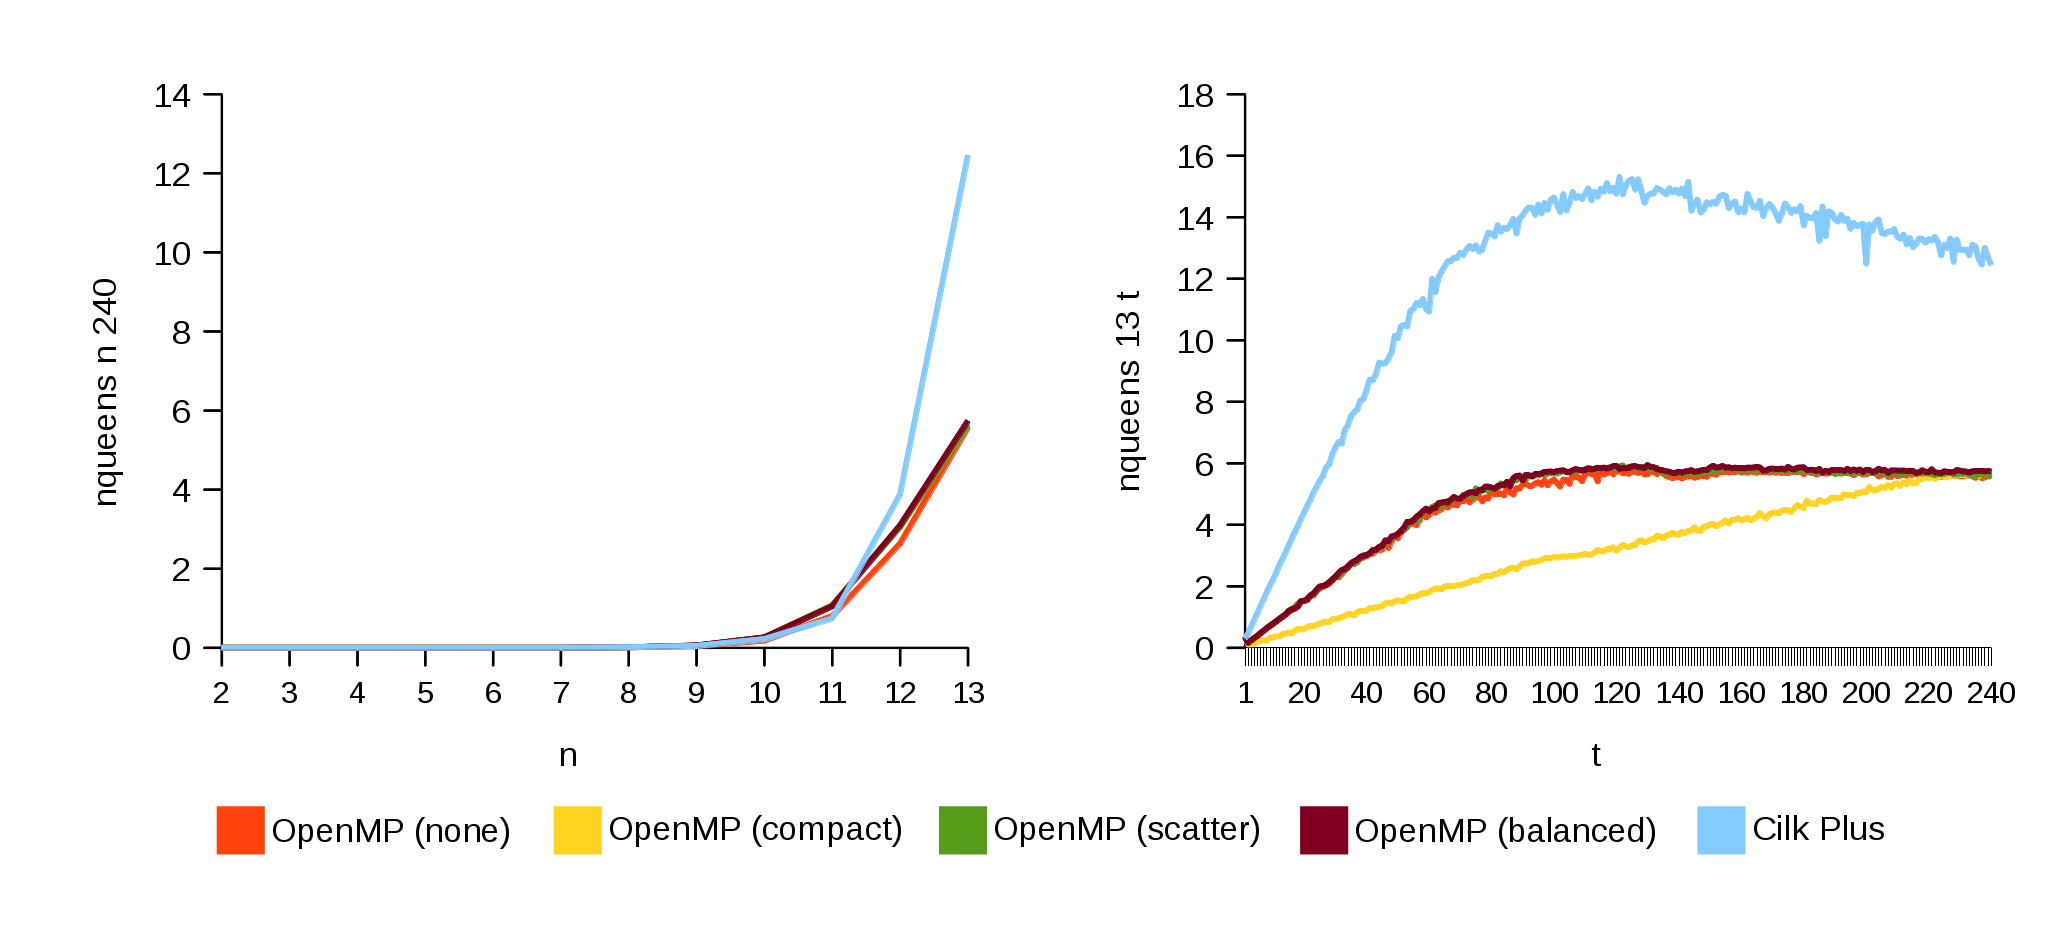
\includegraphics[width=\linewidth]{../../charts/mic/nqueens_speedup}
	\caption{Speedup of the N-Queens benchmark on the Xeon Phi.}
	\label{Fig:nqueensmicspeedup}
\end{figure}

Disabling auto-vectorisation appeared to have no impact on performance, which is largely in line with the finding of Cramer \textit{et al.}\cite{Cramer12}, who observed negligible performance benefits of vectorisation in their benchmark. They found that the performance difference between the vectorised and non-vectorised version of their benchmark narrows as more threads were used, until there was almost no difference at \(t=240\).

\subsection{Cut-off} \label{Sec:evalnqueenscutoff}

The cut-off variant of the N-Queens benchmark is often presented in the literature. This version prevents the spawning of new tasks after a particular level of the task graph, specified with the \(c\) parameter. A cut-off of \(c=13\) is equivalent to the N-Queens benchmark without cut-off, and \(c=0\) is executed as a fully serial program. The results presented below were produced by running the N-Queens cut-off variant on the host machine and Xeon Phi with \(n=13\) while using the maximum number of threads available on each device.

\subsubsection{Host}

Figure \ref{Fig:nqueenscutoffhost} shows the performance of the N-Queens benchmark on the host machine for difference values of \(c\). The left chart shows the execution time and the right chart shows the speedup. With \(c=0\), the benchmark executes in serial, and all parallel versions perform worse than the true serial implementation. However, this drops immediately when the cut-off is raised to 1. This is caused by the parallel for-loop now passing the cut-off test once, and spawning enough tasks to be used by all 32 available threads. The actual speedup, however, is closer to 10 times due to overhead. As \(c\) increases further, this rises to a maximum of 12 times speedup for Cilk Plus and OpenMP with compact thread affinity. The cause of the difference between the thread affinities is not clear, but all affinities show the same short-lived performance drop when \(c=3\). Cilk Plus shows the same feature at a higher value. As expected, when \(c\) approaches 13 and the tasks become more fine-grained, performance drops.
\noindent
\begin{figure}[t!]
	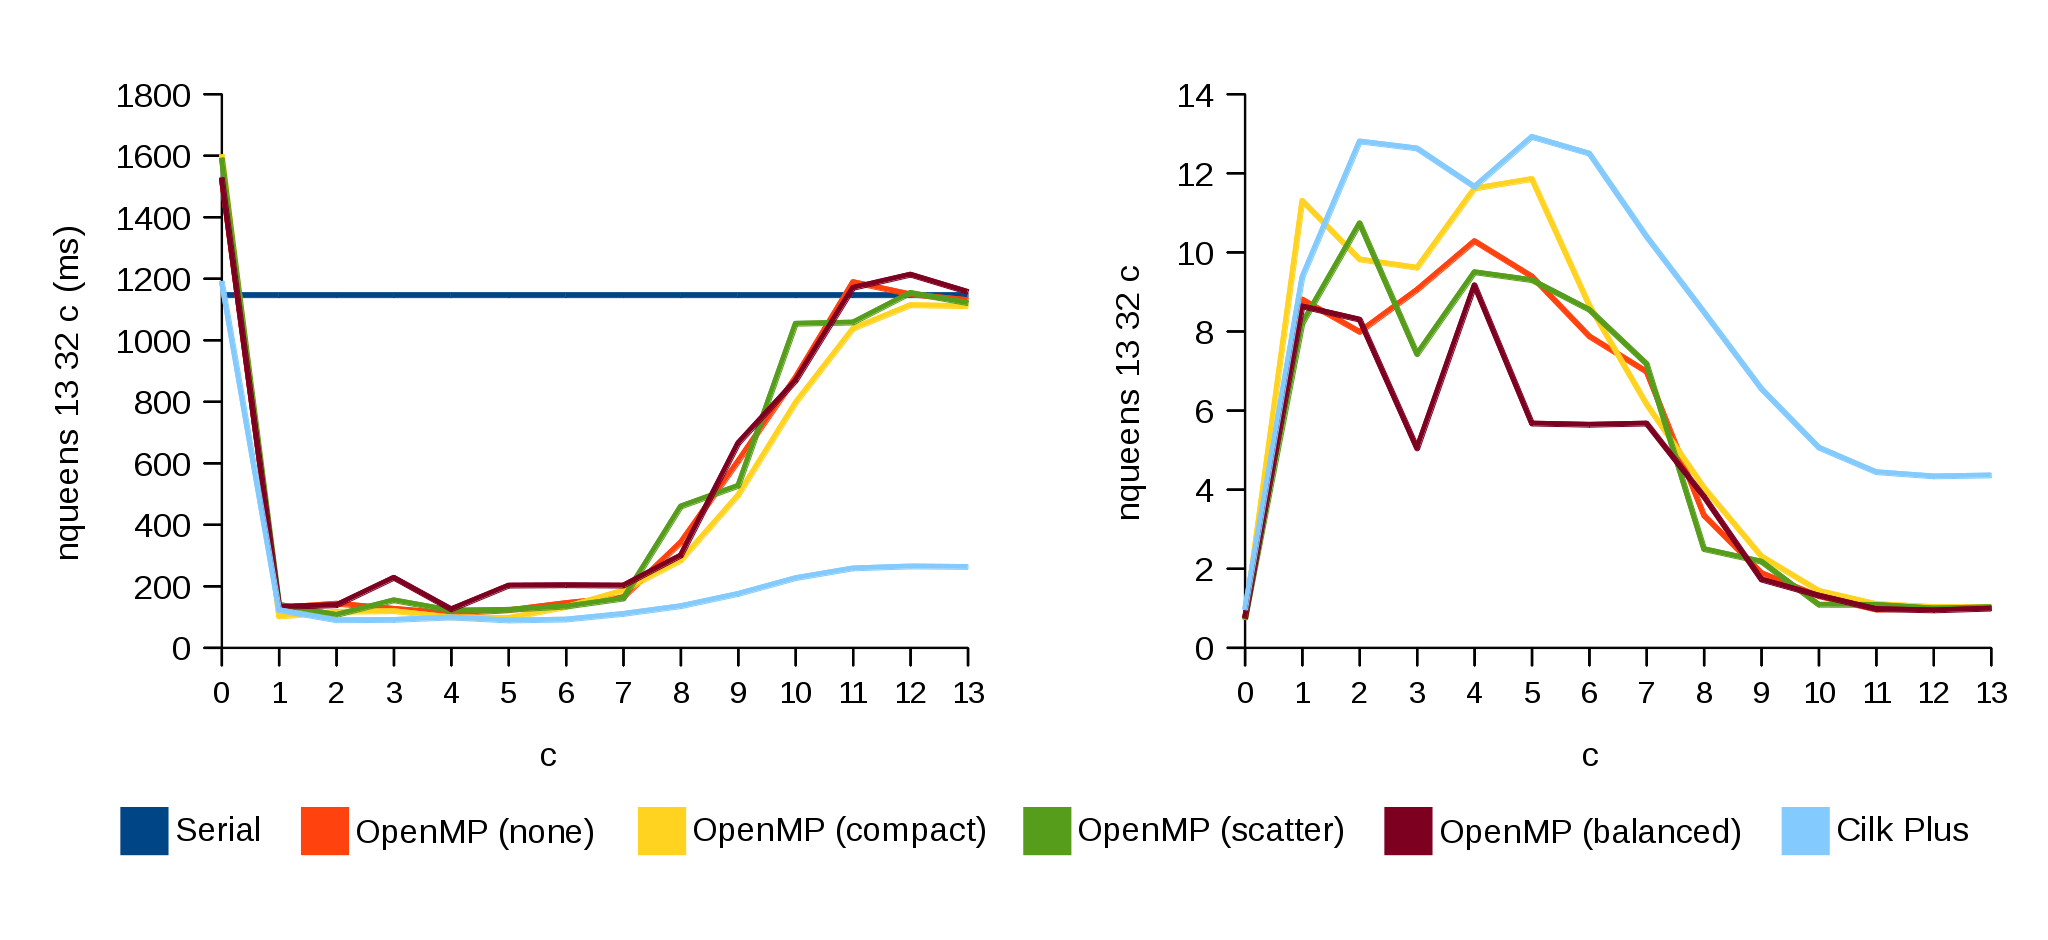
\includegraphics[width=\linewidth]{../../charts/intel64/nqueens_cutoff}
	\caption{Execution time (left) and speedup (right) of the N-Queens benchmark with cut-off on the host machine.}
	\label{Fig:nqueenscutoffhost}
\end{figure}

\subsubsection{Xeon Phi}
Figure \ref{Fig:nqueenscutoffmic} shows the same trial conducted on the Xeon Phi with 240 threads. The same immediate drop in execution time is shown, causing speedup of around 2.5 times for OpenMP with compact, scatter and balanced thread affinity. Setting no thread affinity appears to cause a major drop in performance, and Cilk Plus similarly underperforms for values of \(c\) in the middle of the trial range. However, Cilk Plus is characterised by a longer tail on its speedup, levelling out at around 1.5 times speedup when the maximum cut-off is used. This is consistent with other benchmarks that have shown Cilk Plus to exhibit much lower tasking overhead when compared to OpenMP. It may also be caused by the use of \verb!cilk_for!, rather than manually spawning new tasks, as one is forced to do in OpenMP. The same performance drop when \(c=3\) on the host machine is also present here for OpenMP, suggesting it may be caused by an unbalanced task-graph, a feature of the N-Queens benchmark raised by Duran \textit{et al.}\cite{Duran09}.
\noindent
\begin{figure}[t!]
	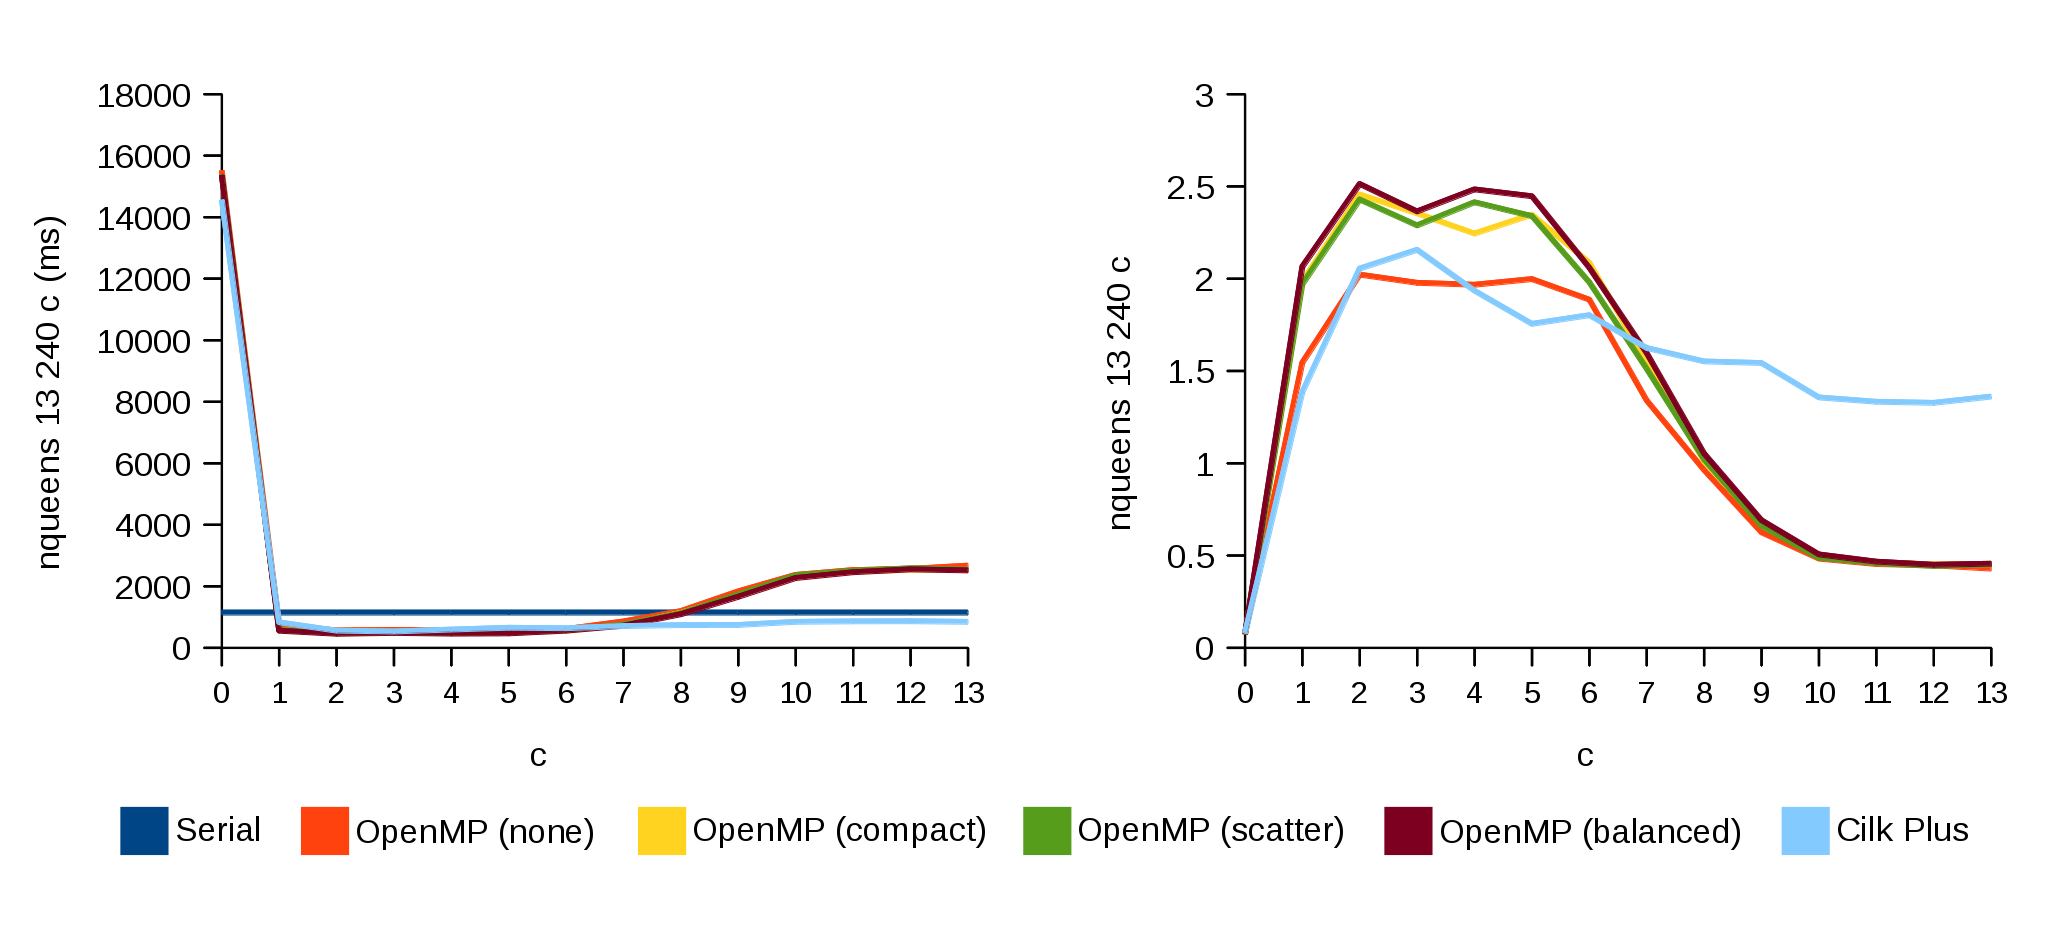
\includegraphics[width=\linewidth]{../../charts/mic/nqueens_cutoff}
	\caption{Execution time (left) and speedup (right) of the N-Queens benchmark with cut-off on the Xeon Phi.}
	\label{Fig:nqueenscutoffmic}
\end{figure}

\subsubsection{Comparison}
In both cut-off benchmarks, the \(13 \times 13\) N-Queens benchmark performs best with a cut-off value between 2 and 5. Interestingly, the results also indicate that even cut-off values produce better speed-up due to more balanced work-loads. This phenomenon is less pronounced when using Cilk Plus. Using the proper cut-off value on the host machine produces around 10 times speedup compared to using no cut-off, a result similar to that found by Duran \textit{et al.}\cite{Duran09}. However, the effect of the cut-off strategy for the N-Queens benchmark on the Xeon Phi is much weaker. The Xeon Phi sees almost no difference in performance, possibly due to several aspects of the device which allow it to better handle fine-grained parallelism, such as the high-speed bi-directional ring interconnect and system-wide coherent L2 cache. The greater coarseness created by the cut-off may also be more beneficial on the host machine because it minimises the amount of communication between cores that must be conducted across the motherboard rather than within a single chip. Future work could involve testing the most performant cut-off values discovered here with different numbers of threads.

\section{Unbalanced Tree Search} \label{Sec:evaluts}

The UTS benchmark used in this project tests the impact of increasingly coarse task granularity on a procedurally generated tree structure. It differs from other benchmarks discussed in this chapter because both the work-load and granularity increase with the \(g\) parameter, since this only changes the number of iterations of the SHA-1 hash function when each node is spawned. As a relatively recent benchmark, there are fewer published experiments using it than others in this report. In this section, the existing literature is referenced when relevant to highlight particular features present in the data produced for this project.

\subsubsection{Host}

Figure \ref{Fig:utshosttime} (left) shows the results produced by the UTS benchmark on the host machine. The x-axis shows the granularity parameter \(g\) increasing through the trial range of \([1,10]\). As expected, increases in \(g\) cause progressively higher execution times due to the additional work-load. Other than for direct comparison between hardware, therefore, the figures showing execution times for this benchmark are not as useful as those showing speedup over the serial version. Figure \ref{Fig:utshostspeedup} (left) shows the speedup of the same trials. The clear trend for the Cilk Plus implementation is towards better speedup as the task coarseness and work-load increase. One would not expect this trend to change, since effective load-balancing should provide continued benefits for parallel implementations. Comparatively, the speedup produced by OpenMP for different values of \(g\) is much less predictable. Their trend is still clearly positive, but no clear difference in the performance of different thread affinities emerged when using 32 threads. All parallel trials produced good speedup, especially Cilk Plus, which achieved around a 15 times performance improvement over the serial version when \(g=10\). OpenMP produced a wide range of performance improvements over the serial version, between and 4-10 times, but this is still an impressive gain compared to other benchmarks conducted on the host machine.
\noindent
\begin{figure}[t!]
	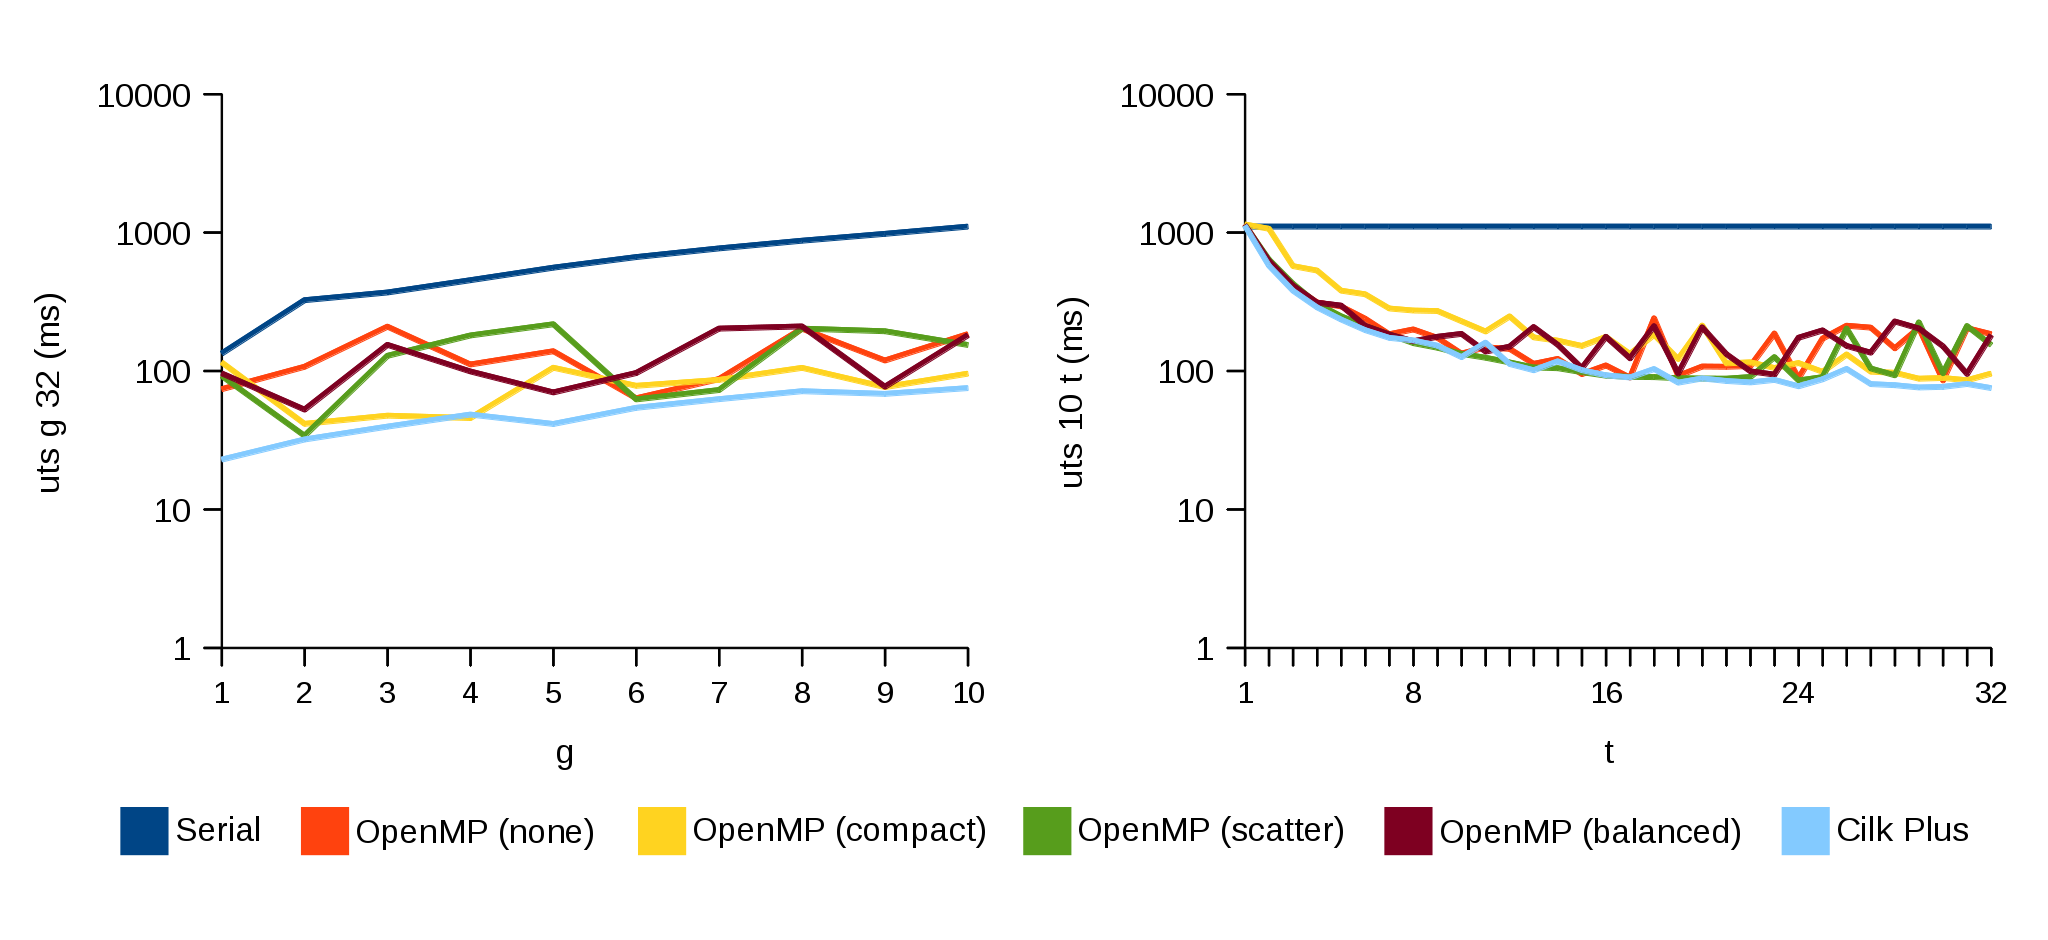
\includegraphics[width=\linewidth]{../../charts/intel64/uts_time}
	\caption{Execution time (milliseconds) of the UTS benchmark on the host machine.}
	\label{Fig:utshosttime}
\end{figure}
\noindent
\begin{figure}[t!]
	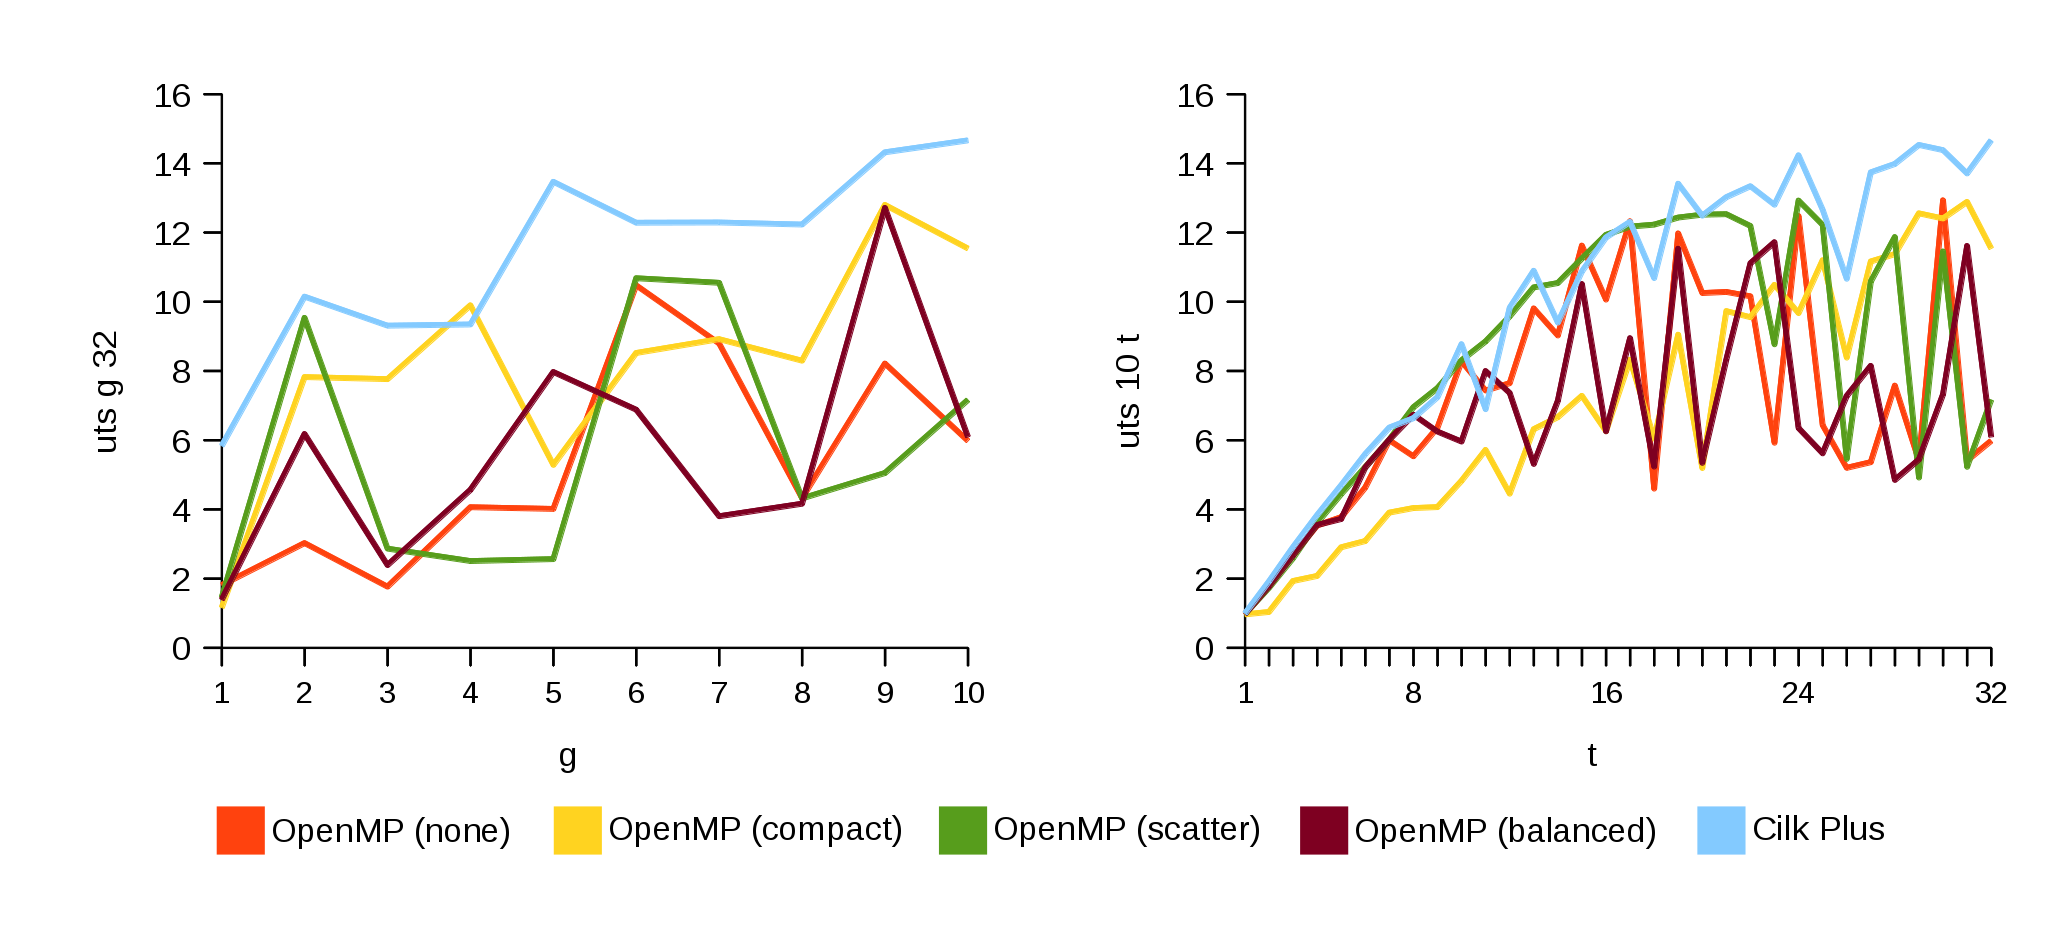
\includegraphics[width=\linewidth]{../../charts/intel64/uts_speedup}
	\caption{Speedup of the UTS benchmark on the host machine.}
	\label{Fig:utshostspeedup}
\end{figure}

Figure \ref{Fig:utshosttime} (right) shows the results produced by the UTS benchmark when the maximum value of \(g\) in the trial range was used and the number of available threads increased for 1 to 32. Figure \ref{Fig:utshostspeedup} (right) shows the speedup relative to the serial version of the same trials. For all values of \(t>1\), every parallel version achieved real speedup, which continued to increase as more threads were made available. Cilk Plus again outperformed OpenMP, continually seeing better speedup over the serial version as \(t\) was increased. OpenMP likewise produced the same wild variations in speedup seen in the previous chart, with the notable difference that setting thread affinity to compact produces better relative performance as \(t\) approaches full thread utilisation on the host machine. Indeed, compact affinity achieves speedup almost at parity with Cilk Plus at 30 threads. This suggests that the increased coarseness of the task granularity compared to earlier benchmarks benefits OpenMP more than Cilk Plus. Interestingly, most trials experienced a drop in performance when 26 threads were used. OpenMP using the balanced thread affinity is the notable exception to this.
\noindent
\begin{figure}[t!]
	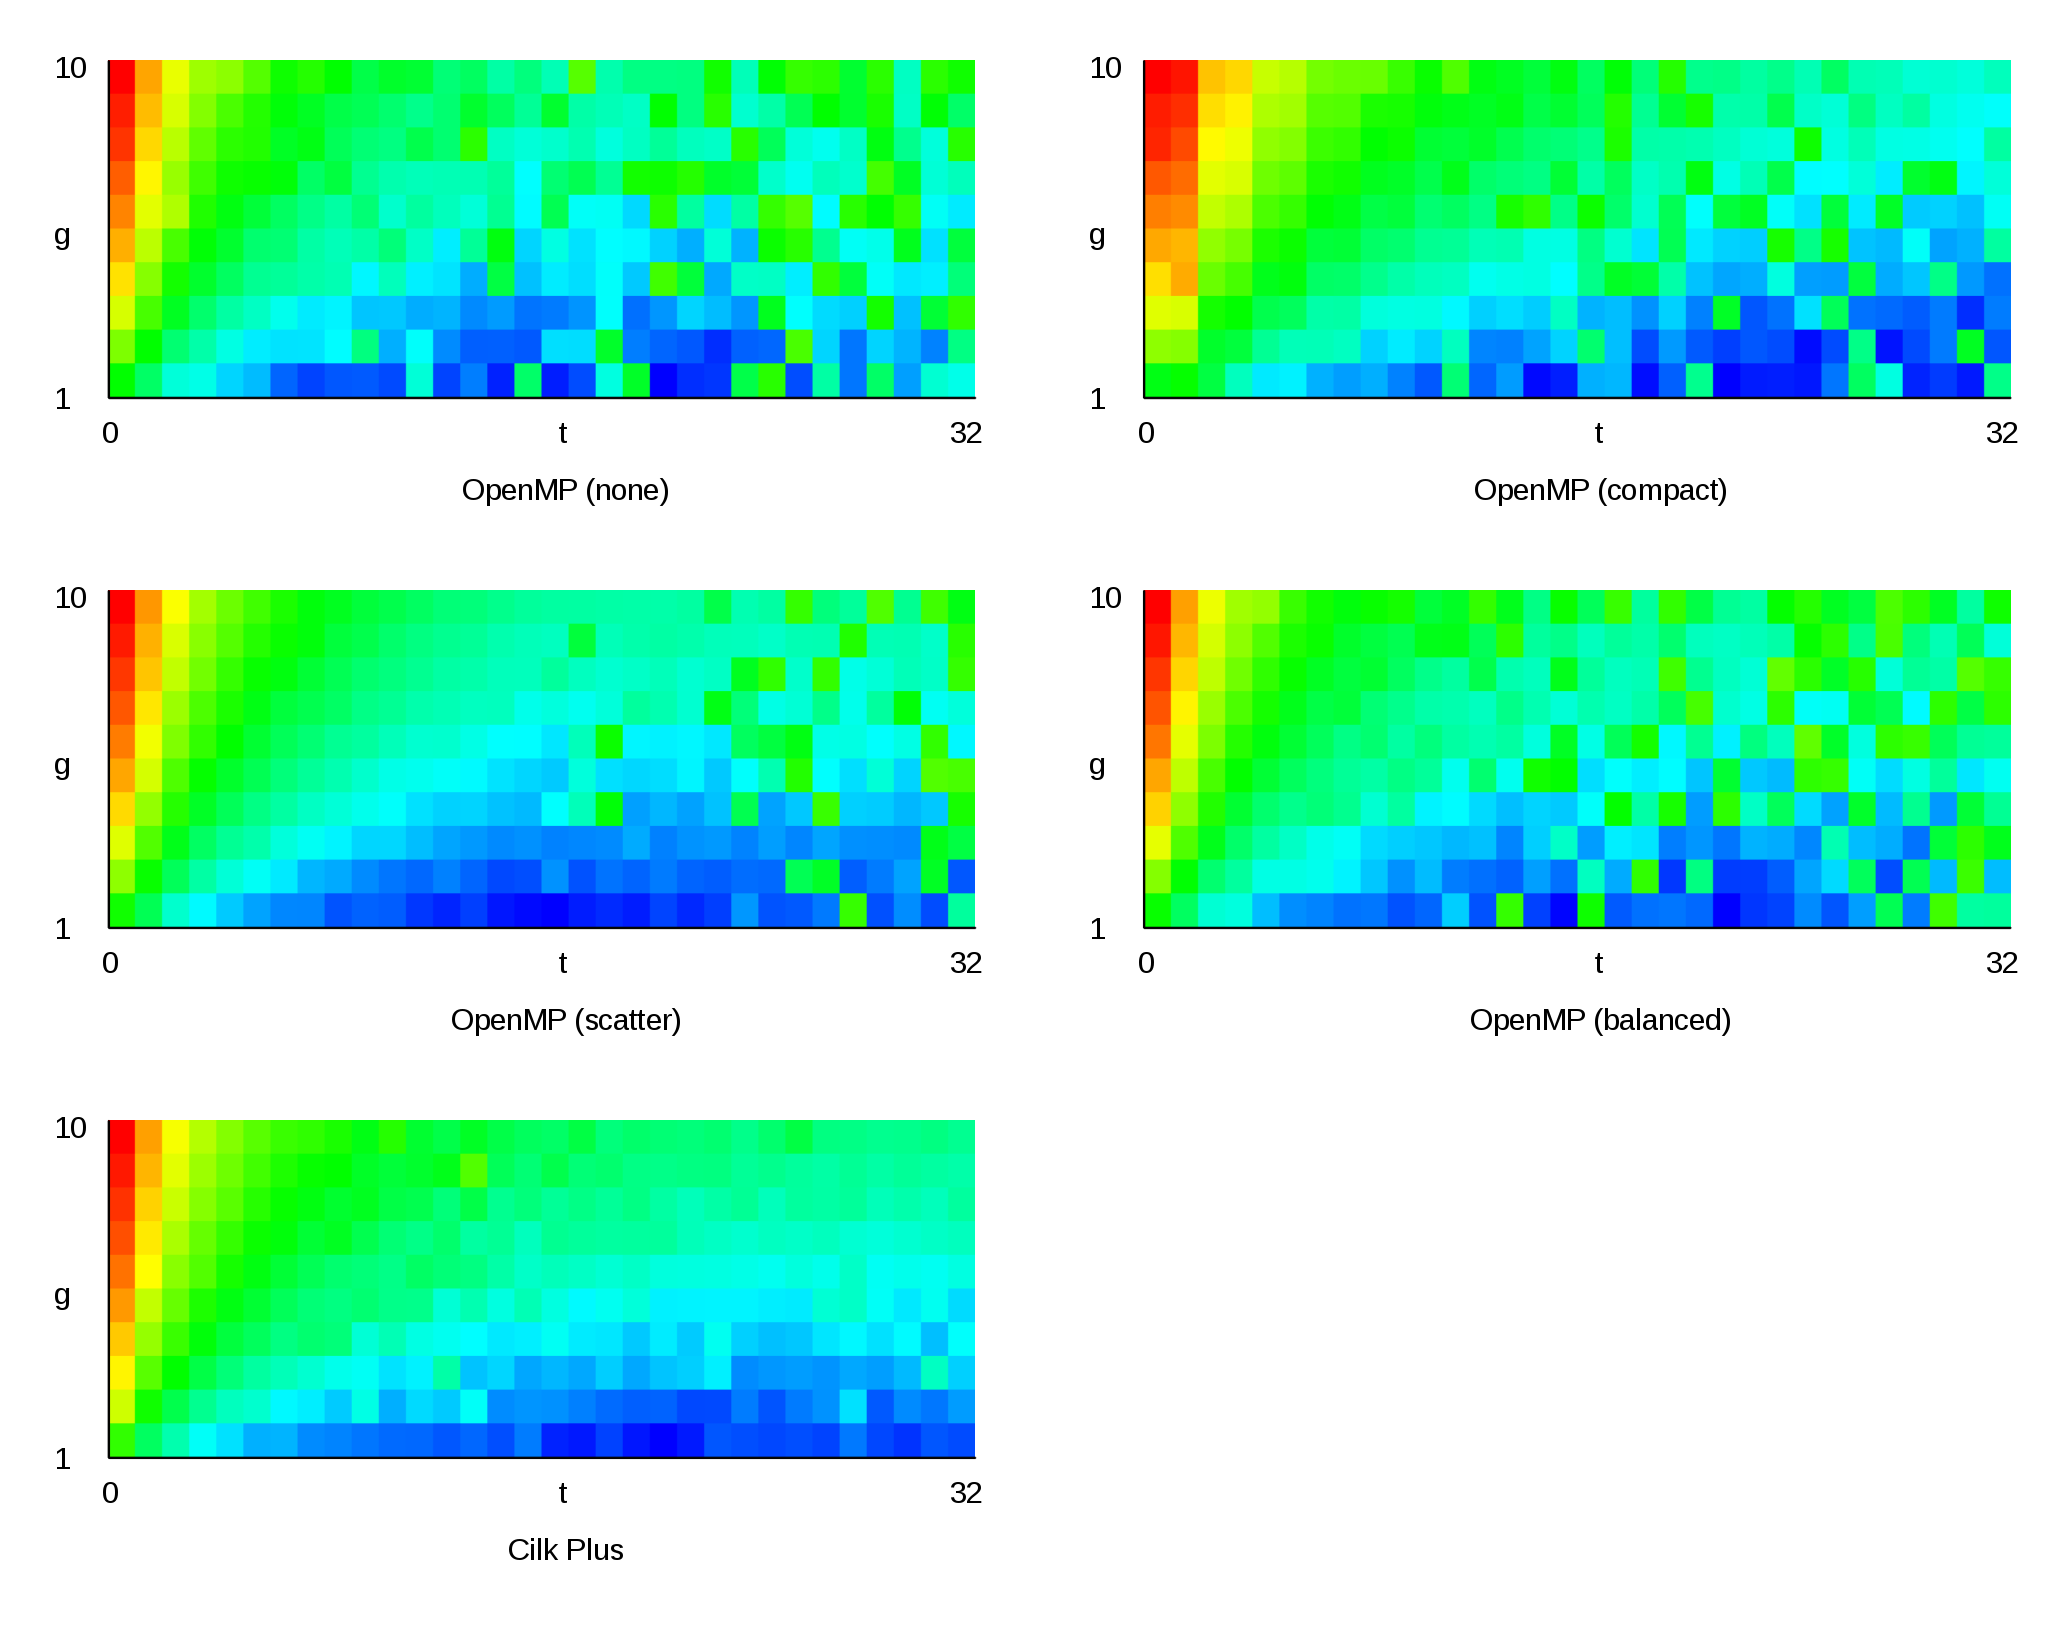
\includegraphics[width=\linewidth]{../../heatmaps/intel64/uts}
	\caption{Heatmaps showing performance spread of the UTS benchmark for different combinations of n and t on the host machine.}
	\label{Fig:utshostheatmap}
\end{figure}

Figure \ref{Fig:utshostheatmap} shows the heatmaps produced by running the UTS benchmark with all combinations of \(g\) and \(t\) on the host machine. Compared to other benchmarks discussed in this chapter, the figures presented here show a distinct linearity in their colour gradients. This suggests strong scaling, since there is equivalence in performance for different values of \(g\) and \(t\) in a wide range. Notably, the colour gradient becomes more shallow as \(t\) increases, further suggesting that the UTS benchmark scales well to additional threads and workloads. An interesting feature that also appeared in other benchmarks is the level of noise in the results for OpenMP trials. Cilk Plus is characterised by much smoother colour gradients, with less noise at higher values of  \(t\), possibly due to its superior load-balancing capabilities.

\subsubsection{Xeon Phi}

Figure \ref{Fig:utsmictime} (left) shows the results produced by conducting the same set of trials on the Xeon Phi with 240 threads. As in all other benchmarks, the serial version performs worse than on the host machine. The parallel implementations also maintain a much shallower angle throughout the trials as \(g\) increases, indicating weaker scaling. However, they still produce a large performance improvement over the serial version at all levels of \(g\). Figure \ref{Fig:utsmicspeedup} (left) shows that that the maximum speedup achieved was around 22 times. Surprisingly, OpenMP outperformed Cilk Plus for most values of \(g\). This difference becomes more pronounced as \(g\) increases further, possibly because Cilk Plus' efficient scheduler has less impact when tasks are more coarse. Despite this, Cilk Plus saw around a 12 times speedup when \(g=10\). Setting no thread affinity in OpenMP again caused the worst performance of the alternatives on the Xeon Phi, but the general trend appears to be linear performance gains for OpenMP as a whole.
\noindent
\begin{figure}[t!]
	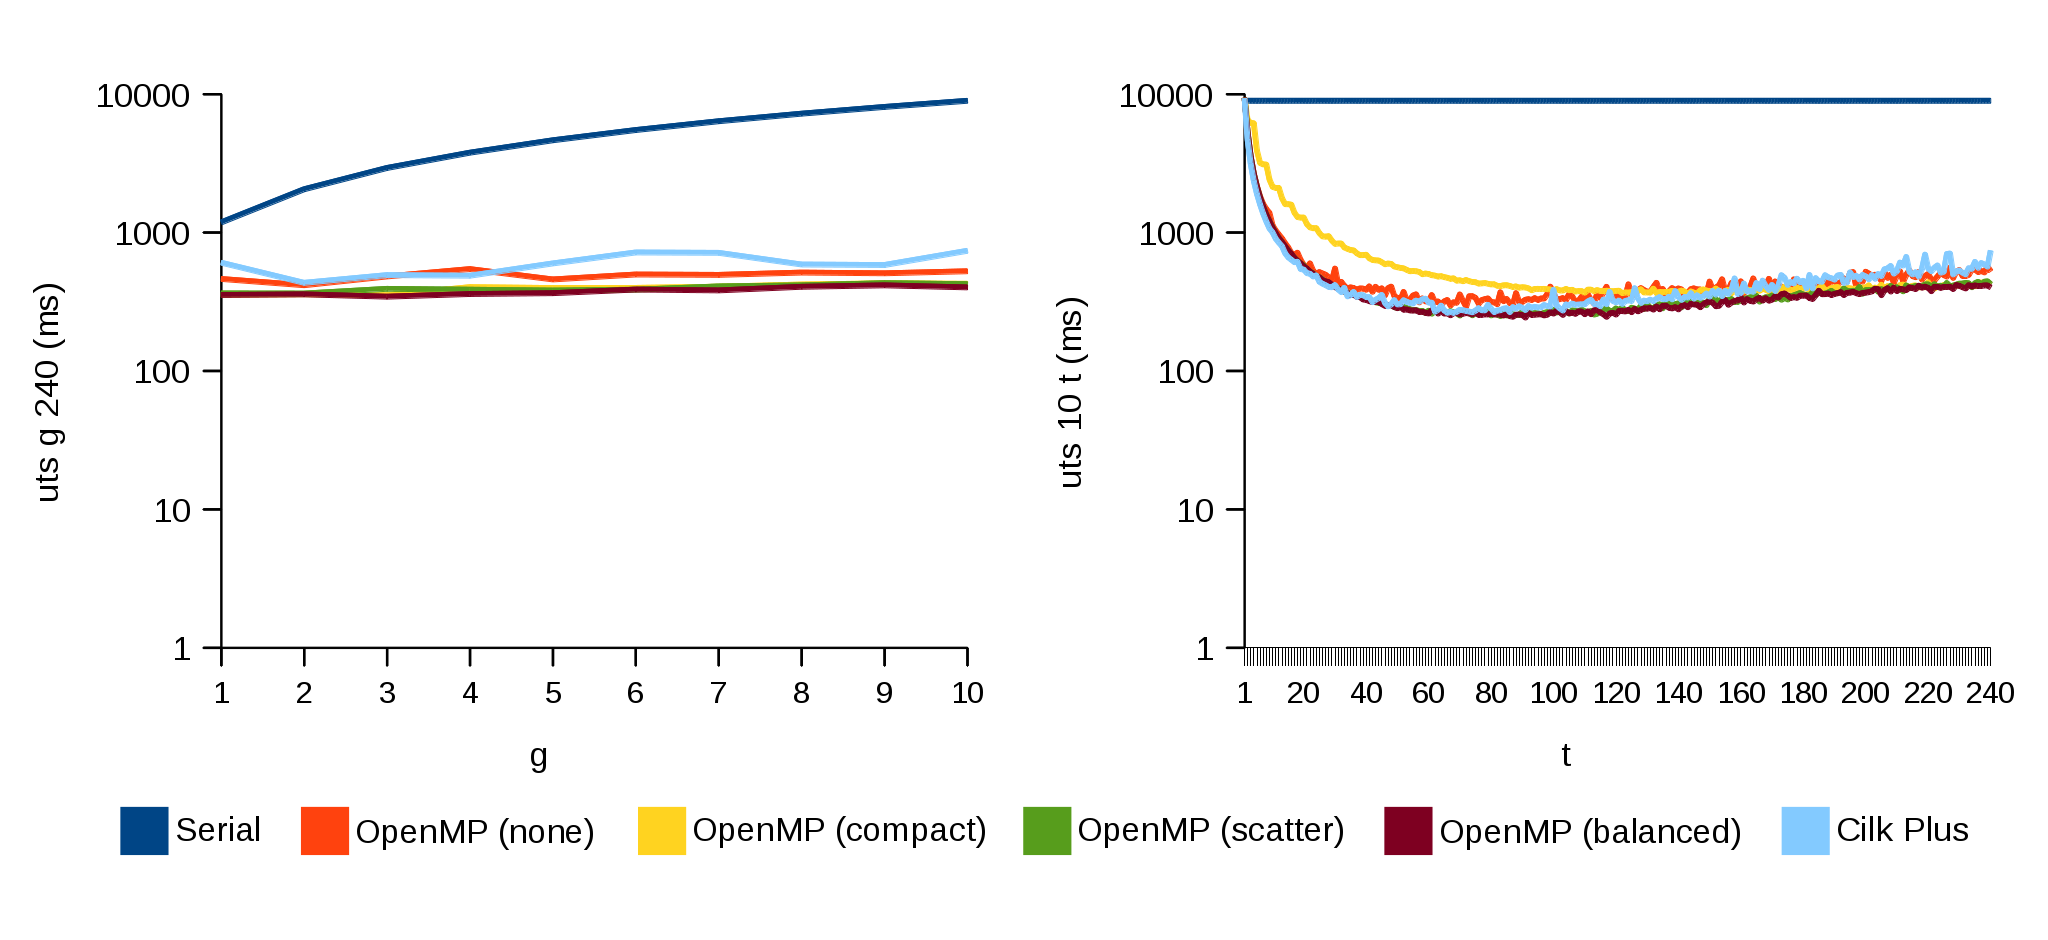
\includegraphics[width=\linewidth]{../../charts/mic/uts_time}
	\caption{Execution time (milliseconds) of the UTS benchmark on the Xeon Phi.}
	\label{Fig:utsmictime}
\end{figure}
\noindent
\begin{figure}[t!]
	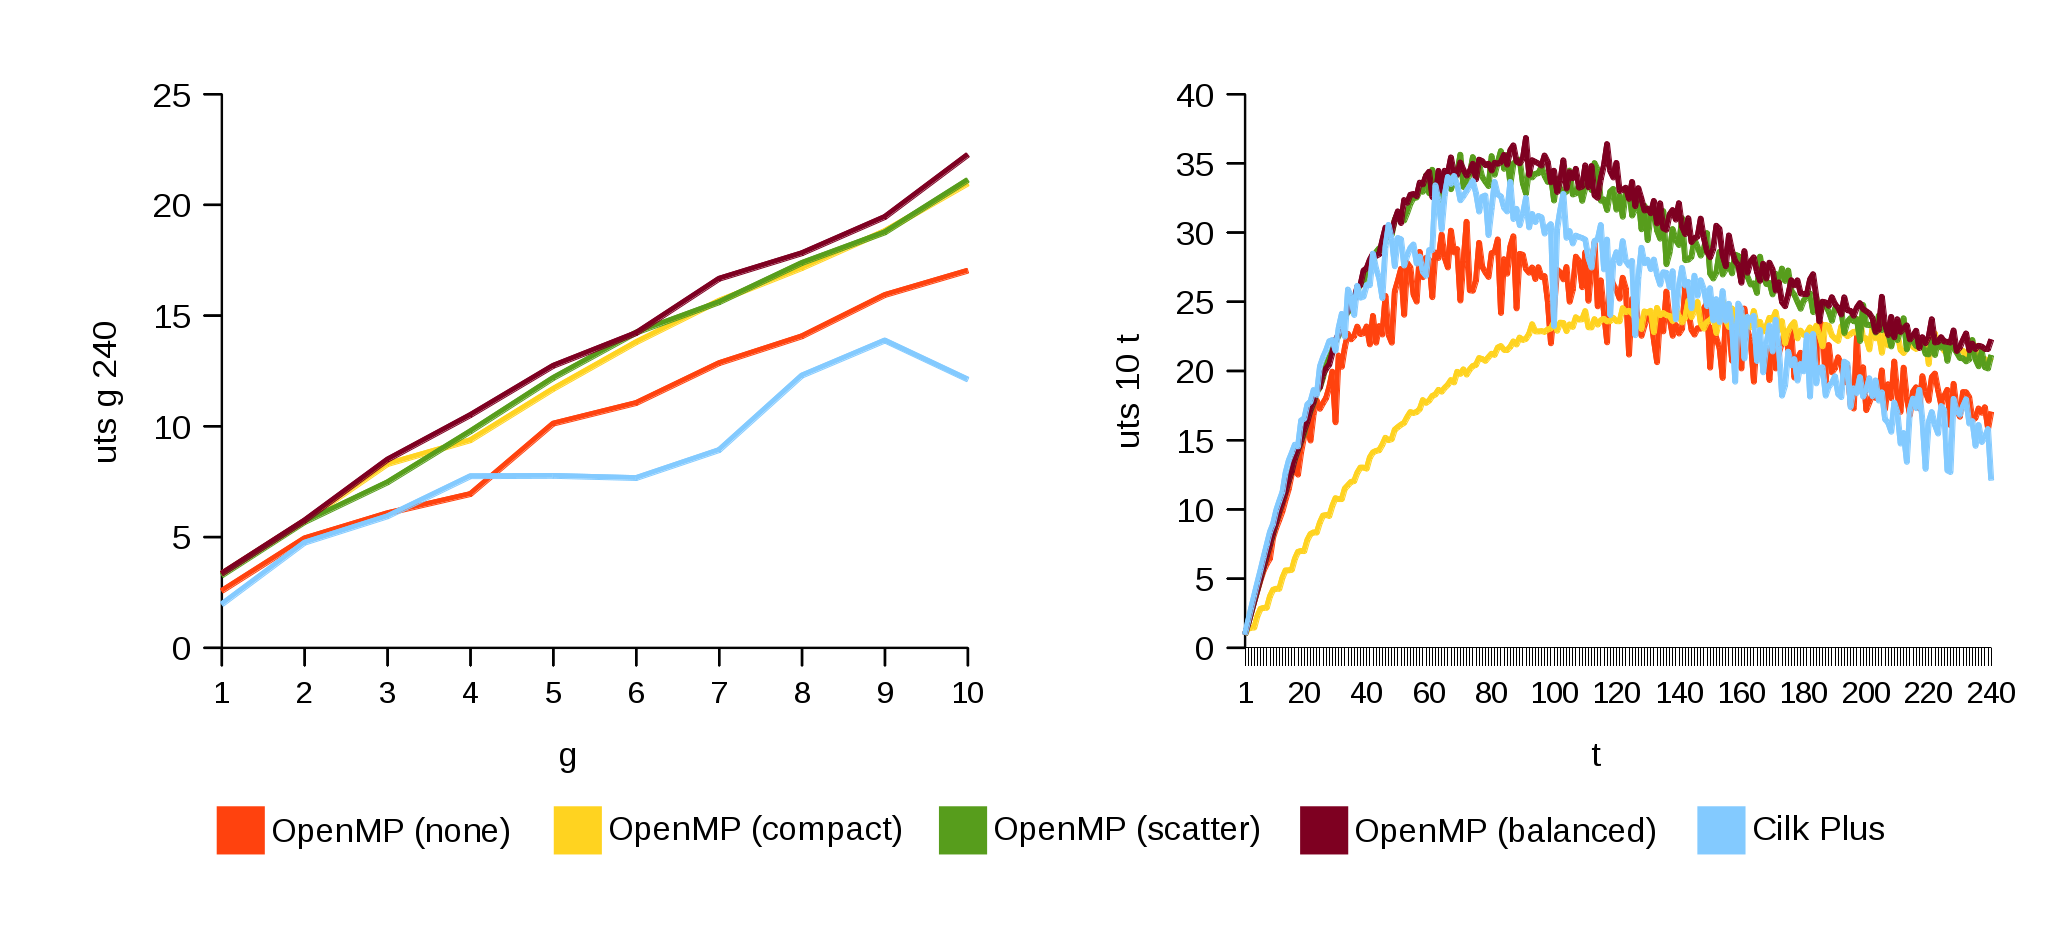
\includegraphics[width=\linewidth]{../../charts/mic/uts_speedup}
	\caption{Speedup of the UTS benchmark on the Xeon Phi.}
	\label{Fig:utsmicspeedup}
\end{figure}

Figure \ref{Fig:utsmictime} (right) shows the results from running the UTS benchmark with maximum task coarseness with different numbers of available threads. As in N-Queens on the Xeon Phi, the parallel framework provided their greatest benefit when fewer threads were used. OpenMP with scatter or balanced thread affinity achieved the best speedup of any trial, at around 35 times with 80 threads. Saule and Catalyurek\cite{Saule12} found exactly the same trend with their own unbalanced tree benchmark; peak performance was achieved with around 60-80 threads, and OpenMP outperformed Cilk Plus. Beyond this number of threads, they found that the speedup gained by Cilk Plus dropped more rapidly. However, their results also show Cilk Plus achieving greater speedup when task coarseness increased, the opposite to what is presented here. The results produced for this  report also show scatter and balanced OpenMP affinities performing consistently better than the alternatives, until \(t\) approaches maximum thread utilisation, at which point the compact affinity converges on the same speedup after earlier underperformance.
\noindent
\begin{figure}[t!]
	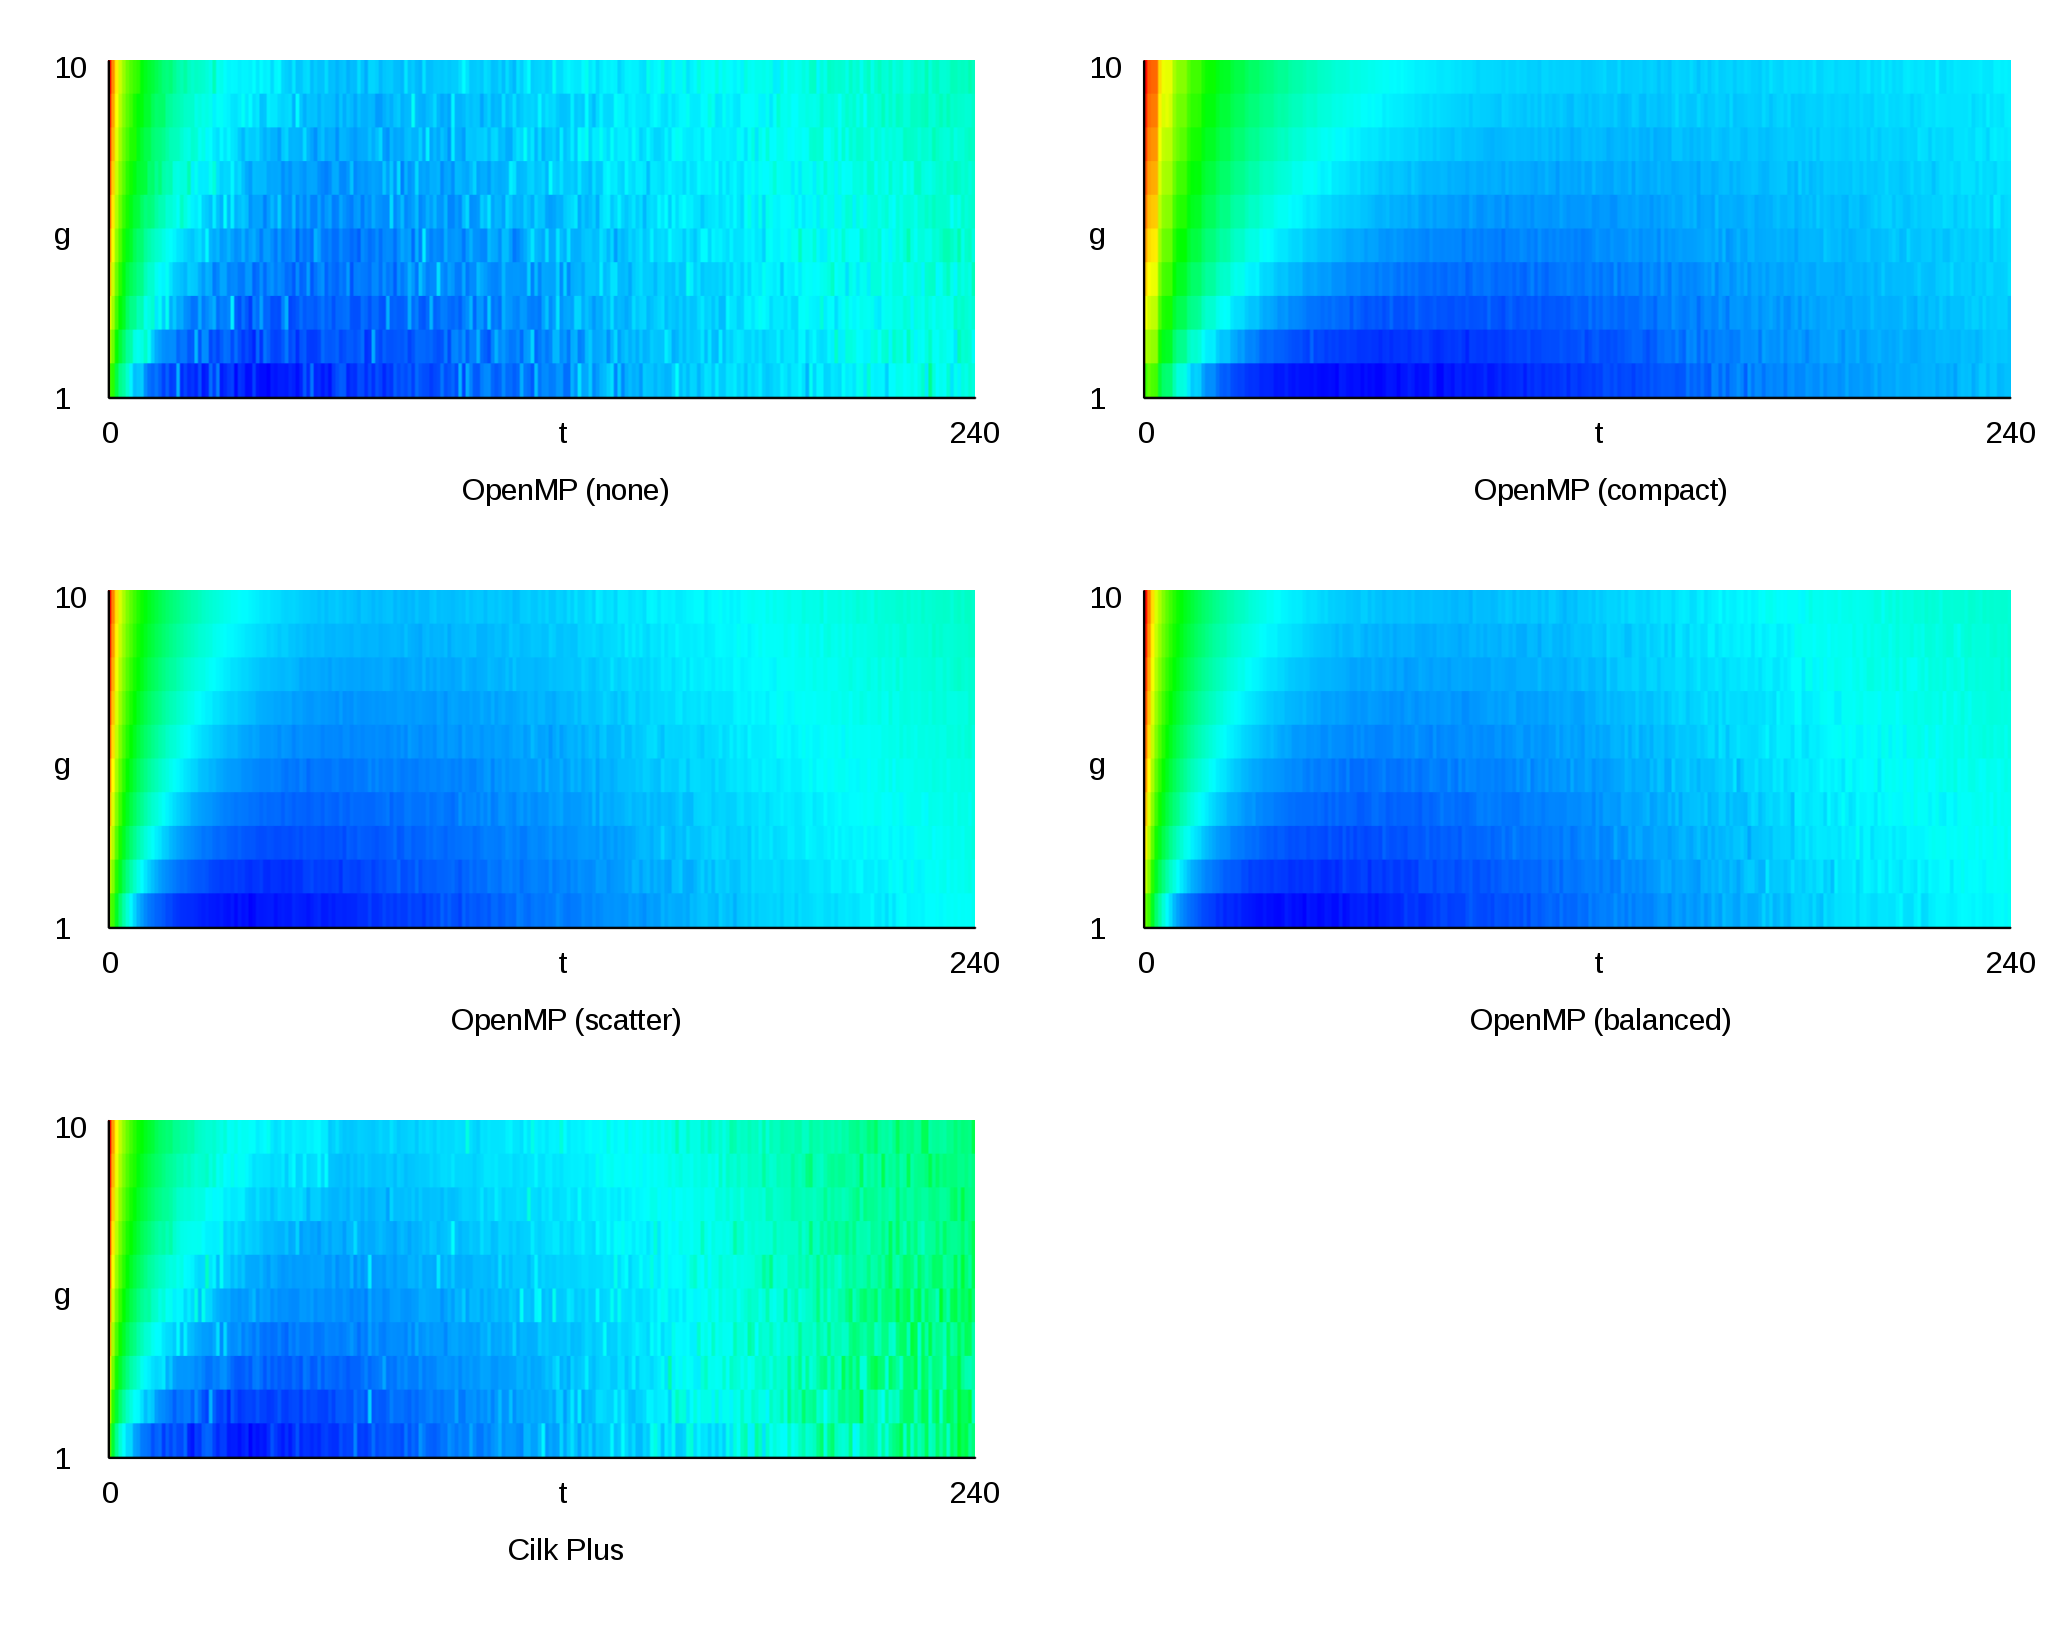
\includegraphics[width=\linewidth]{../../heatmaps/mic/uts}
	\caption{Heatmaps showing performance spread of the UTS benchmark for different combinations of n and t on the Xeon Phi.}
	\label{Fig:utsmicheatmap}
\end{figure}

Figure \ref{Fig:utsmicheatmap} shows the heatmaps produced by executing the UTS benchmark on the Xeon Phi for every combination of \(g\) and \(t\). They show an extremely interesting trend, which could be key to achieving maximum parallel performance on the Xeon Phi. For all frameworks, the best performance lies within particular ranges of \(g\) and \(t\), and increasing either of these parameters by too much decreases performance. These results show that, as one would expect, too much work for too few threads causes inefficiency, but also that too little work for too many threads produces the same effect. This feature does not appear as clearly in the results of other benchmarks presented in this report, but the same trend may have been visible in the N-Queens benchmark if higher values of \(n\) were tested. Ultimately, it seems that workloads must be sufficiently large for the Xeon Phi to provide the best performance gains, suggesting that the host machine's superiority in previous benchmarks may be partially due to insufficiently large workloads resulting from low input values.

\chapter{Conclusion} \label{Sec:conclusion}

\section{Summary and Recommendations}

In most of the results presented in this report, the Xeon Phi demonstrated better scaling of parallel applications than the two Xeons in the host machine, but this advantage should be taken in the context of lower overall performance in every trial. Trends observed in the N-Queens and UTS benchmarks suggest that the Xeon Phi may be able to achieve better performance than the host machine in applications producing very large work-loads, but that small work-loads actually suffer in the highly parallel environment of the MIC architecture. Examples of other authors reaching the same conclusion are rare, possibly due to Intel not positioning the Xeon and Xeon Phi as competitors. Although this project was not intended as a direct comparison of performance between the two devices, distinct performance patterns did emerge, and careful selection of which hardware is used for certain applications may yield lower execution times.

Taken together, the benchmarking results and the wider literature suggest that hardware-specific optimisations can produce significant benefits, but some more general rules-of-thumb also emerged. The cut-off variants of Fibonacci and N-Queens performed much better than their respective standard versions, boosting the speedup achieved by several times. There did not appear to be a specific cut-off value that provided the best speedup in either trial, but the best values actually emerged as a range. Likewise, the UTS benchmark resulted in a range of task-granularity appearing to provide some benefit, but also revealed that the effectiveness of this approach may also be linked to the number of available threads.

Cilk is sometimes reported in the literature as a panacea for poor performance in parallel applications\cite{Blumofe95}\cite{Dailey01}\cite{Leiserson09}, demonstrating superior task-scheduling that results in better load-balancing than alternative frameworks, while also featuring much lower task creation overhead than OpenMP. While Cilk Plus did provide better speedup than OpenMP in most trials, the latter should not be discounted; OpenMP scaled better on the Xeon Phi when almost all threads were used. Using the compact thread affinity, in particular, provided better speedup than the alternatives for number of threads approaching those available on both the host machine and Xeon Phi. The data do not suggest, however, that thread affinity has as significant an impact on performance as does the choice of framework, with the exception of setting no affinity, which clearly underperformed in some benchmarks conducted on the Xeon Phi. See in particular the results of the Fibonacci benchmark in Section \ref{Sec:evalfib} and the merge sort benchmark in Section \ref{Sec:evalmsort}.

Intel's literature on writing programs for its hardware states that full use of a device's SIMD units are key to achieving maximum parallel speedup\cite{overviewxeonandxeonphi}. This project used the auto-vectorisation capabilities of the Intel C++ Compiler to evaluate its impact on performance. The auto-vectorsation of N-Queens performed by the Intel compiler fell short of the performance reported by Jeffers and Reinders\cite{Jeffers13}, who recommend careful tuning of code to exploit the vector units available on the Xeon Phi. The application of manual vectorisation to a suitable benchmark, such as matrix multiplication, may provide a better comparison in future work. If maximum exploitation of the hardware is necessary, the results of the power-of-two merge sort benchmark suggest that manual load-balancing provides little to no benefit, particularly in applications with fine-grained tasks. The data suggest that Cilk Plus impressively handles highly unbalanced task-graphs, such as those produced by the UTS benchmark -- this feature of the language has been noted by other authors \cite{Tousimojarad14} -- and time could be better spent conducting manual vectorisation.

\section{Achievements}

The achievements of this project, both technical and personal, are listed below.
\begin{itemize}
	\item Learned to use Cilk Plus and OpenMP.
	\item Produced data comparing the performance of Cilk Plus and OpenMP on different hardware.
	\item Learned several methods of overcoming race conditions.
	\item Gained experience with more highly parallel hardware after earlier exposure to the HPC Wales supercomputing cluster.
	\item Gained experience managing large data sets.
	\item Gained familiarity with Intel hardware and tools.
	\item Gained an appreciation for the capabilities of Intel Xeon and Xeon Phi.
	\item Presented results-based recommendations for achieving greater parallel performance when using task parallelism on Intel Xeon and Xeon Phi.
\end{itemize}

\section{Criticism of Methodology}

An issue encountered during the course of this project was an over-abundance of data to manage and analyse. This may have been caused by testing too many benchmarks, some producing very similar results. Careful selection of parameters passed to the UTS benchmark may have made it possible to replicate results generated by the Fibonacci, merge sort and N-Queens benchmarks using only one program. This should be considered in future work.

Additionally, confusion in the early stages of the project over its focus reduced the amount of time available to conduct some core aspects of the work, and a lack of clear goals harmed the usefulness of the results obtained. The scope of the project ultimately proved to be too broad, and focusing on a single hardware device, such as the Xeon Phi, may have allowed more time for hardware-specific tests to be developed. Focusing on a single device may also have left time for a more detailed evaluation of the existing results, and particular aspects affecting performance identified. Two alternative approaches may have proven useful: micro-benchmarks used to test particular aspects of the hardware in tightly controlled trials, and the use of Cilk Plus and OpenMP to write a real application. The former approach may have helped to reduce the noise that appeared in some results, particularly those produced on the host machine, and the latter would have provided more focus at an early stage and provided more opportunity for discussion of the engineering aspects of working with task parallelism.

Regarding the visualisation of results, in most cases the heatmaps generated from the benchmarks did not provide the degree of additional insight that was hoped for. The time taken to perform computations for every combination of inputs was probably not worthwhile when the final usefulness of the heatmaps is considered. On the other hand, the heatmaps generated from the UTS results provided a good visual representation of the impact of task granularity and thread utilisation on performance. In future work, it might be possible to avoid the time investment required to produce the heatmaps by first performing lower-resolution sampling of the programs under test to identify the best combination of work-load, task-granularity and thread utilisation.

\section{Future Work}

One obvious area of expansion for this project is the inclusion of more task-centric parallelisation frameworks. Intel Threading Building Blocks (TBB) is a framework that often appears alongside Cilk and OpenMP in similar evaluations, and the large quantity of information, documentation and support for it, especially from Intel, would make this a relatively painless addition. Note however that the inclusion of Intel TBB may require a migration of the existing benchmarks to C++ if comparisons were to remain fair. A more recent development in the field of task parallelism is Wool\cite{woolsite}. Wool is a new C library intended as a fast, low-overhead alternative to existing frameworks. It is still in early stages of development, but experiments conducted with it have found highly competitive results\cite{Podobas15}. Use of the Xeon Phi's offload mode may also be an interesting area of research.

Applying task-parallelism to the development of a real program may lead to more results with more practical application than found in this project. An evaluation on modern hardware of the classes of programs that have traditionally made use of task-centric frameworks, such as chess engines and scientific applications like protein folding\cite{Dailey01}, might give a more realistic indication of the scale of performance one could expect from using those frameworks. 

\bibliography{report.bib}
\bibliographystyle{ieeetr}

\chapter{Appendices} \label{Sec:appendices}
\section{Source Code} \label{App:sourcecode}
Due to the length of the source files, they have been omitted from this appendix, but are included on the CD supplied with this report.

\subsection{timer.h} \label{App:timerh}
See \verb!/benchmarks/host/benchmarks/src/timer.h! on the supplied CD.

\subsection{\purl{fib_serial.c}} \label{App:fibserialc}
See \verb!/benchmarks/host/benchmarks/src/fib/fib_serial.c! on the supplied CD.

\subsection{\purl{fib_omp.c}} \label{App:fibompc}
See \verb!/benchmarks/host/benchmarks/src/fib/fib_omp.c! on the supplied CD.

\subsection{\purl{fib_cilk.c}} \label{App:fibcilkc}
See \verb!/benchmarks/host/benchmarks/src/fib/fib_cilk.c! on the supplied CD.

\subsection{\purl{fib_cutoff_omp.c}} \label{App:fibcutoffompc}
See \verb!/benchmarks/host/benchmarks/src/fib/fib_cutoff_omp.c! on the supplied CD.

\subsection{\purl{fib_cutoff_cilk.c}} \label{App:fibcutoffcilkc}
See \verb!/benchmarks/host/benchmarks/src/fib/fib_cutoff_cilk.c! on the supplied CD.

\subsection{\purl{msort_serial.c}} \label{App:msortserialc}
See \verb!/benchmarks/host/benchmarks/src/msort/msort_serial.c! on the supplied CD.

\subsection{\purl{msort_omp.c}} \label{App:msortompc}
See \verb!/benchmarks/host/benchmarks/src/msort/msort_omp.c! on the supplied CD.

\subsection{\purl{msort_cilk.c}} \label{App:msortcilkc}
See \verb!/benchmarks/host/benchmarks/src/msort/msort_cilk.c! on the supplied CD.

\subsection{\purl{nqueens_serial.c}} \label{App:nqueensserialc}
See \verb!/benchmarks/host/benchmarks/src/nqueens/nqueens_serial.c! on the supplied CD.

\subsection{\purl{nqueens_omp.c}} \label{App:nqueensompc}
See \verb!/benchmarks/host/benchmarks/src/nqueens/nqueens_omp.c! on the supplied CD.

\subsection{\purl{nqueens_cilk.c}} \label{App:nqueenscilkc}
See \verb!/benchmarks/host/benchmarks/src/nqueens/nqueens_cilk.c! on the supplied CD.

\subsection{\purl{nqueens_cutoff_omp.c}} \label{App:nqueenscutoffompc}
See \verb!/benchmarks/host/benchmarks/src/nqueens/nqueens_cutoff_omp.c! on the supplied CD.

\subsection{\purl{nqueens_cutoff_cilk.c}} \label{App:nqueenscutoffcilkc}
See \verb!/benchmarks/host/benchmarks/src/nqueens/nqueens_cutoff_cilk.c! on the supplied CD.

\subsection{\purl{uts_shm_serial.c}} \label{App:utsshmserialc}
See \verb!/benchmarks/host/benchmarks/src/uts/uts_shm_serial.c! on the supplied CD.

\subsection{\purl{uts_shm_omp.c}} \label{App:utsshmompc}
See \verb!/benchmarks/host/benchmarks/src/uts/uts_shm_omp.c! on the supplied CD.

\subsection{\purl{uts_shm_cilk.c}} \label{App:utsshmcilkc}
See \verb!/benchmarks/host/benchmarks/src/uts/uts_shm_cilk.c! on the supplied CD.

\section{Scripts} \label{App:scripts}
Due to the length of the scripts needed to build and run the benchmarks, they have been omitted from this appendix, but are included on the CD supplied with this report.

\subsection{build} \label{App:build}
See \verb!/benchmarks/host/benchmarks/build! on the supplied CD.

\subsection{benchh} \label{App:benchh}
See \verb!/benchmarks/host/benchh! on the supplied CD.

\subsection{benchm} \label{App:benchm}
See \verb!/benchmarks/host/benchm! on the supplied CD.

\subsection{heatmap.py} \label{App:heatmappy}
See \verb!/results/heatmap.py! on the supplied CD.

\section{Results}
Due to the amount of data produced by the benchmarks, the results are omitted from this appendix. Spreadsheets containing the full results are included on the CD supplied with this report.

\end{document}